\documentclass[10pt]{report}
\usepackage{graphicx}
\usepackage{caption}
\usepackage{subcaption}
\usepackage[utf8]{inputenc}
\usepackage[spanish]{babel}
\usepackage{amssymb}
\usepackage{amsmath}
\numberwithin{equation}{chapter}
\usepackage{algorithm}
\numberwithin{algorithm}{chapter}
\floatname{algorithm}{Pseudo-Código}
\usepackage{algpseudocode}
%\usepackage{rotating}
\usepackage[backend=bibtex,bibstyle=authoryear,citestyle=authoryear,sorting=nty,maxnames=1]{biblatex}
\usepackage[colorlinks=true,citecolor=black,linkcolor=black]{hyperref}
\bibliography{BiblioTh7}
\usepackage{makeidx}
\usepackage{tabularx}
\usepackage{longtable}
\usepackage[calcwidth]{titlesec}
%\usepackage{pifont}
\usepackage{marvosym}
%%Para hacer código bonito
\usepackage{listings}
\usepackage{titleps}
\usepackage{lipsum}% just to generate text filler
\newpagestyle{mystyle}[\small]{\headrule
\sethead{\thesection~\sectiontitle}{}{\thepage}
}
\newpagestyle{BibStyle}[\small]{\headrule
\sethead{}{}{}
}
\newpagestyle{ApenStyle}[\small]{\headrule
\sethead{\chaptertitle}{}{\thechapter-\thepage}
}
%%
\makeindex
\DeclareMathOperator{\sinc}{sinc}
\newtheorem {thm}{Teorema}[section]
\newtheorem {defin}{Definición}[section]
\newtheorem {coro}{Corolario}[section]
\newtheorem{assum}{Suposición}[section]
\newtheorem{regla}{Regla}[section]
\newenvironment{proof}[1][Demostracion.-]{\begin{trivlist}\item[\hskip \labelsep {\bfseries #1}]}{\end{trivlist}}
%\renewcommand{\eqref}[1]{\textup{\ref{#1}}}
\newcommand{\bcite}[1]{[\cite{#1}]}
\renewcommand*{\baselinestretch}{1.4}
%\renewcommand{\eqref}{Eq.$\circledast$}
\renewcommand{\labelitemi}{$\circledast$}
\renewcommand{\labelitemii}{$\circleddash$}
\renewcommand{\labelenumi}{\arabic{enumi}.}
\renewcommand{\labelenumii}{\arabic{enumi}.\arabic{enumii}.}
\renewcommand{\labelenumiii}{\arabic{enumi}.\arabic{enumii}.\arabic{enumiii}.}
\newcounter{themysubsubsection}[subsection]
\newcommand{\mysubsubsection}[1]{\noindent\par\addtocounter{themysubsubsection}{1} \thesubsection.\arabic{themysubsubsection}\hspace{2mm}\textit{#1}\par}
\newcommand{\parderiv}[2]{\frac{\partial #1}{\partial #2}}
\newcommand{\deriv}[1]{\frac{d #1}{dt}}
\newcommand{\vect}[1]{\boldsymbol{#1}}
\newcommand{\estp}[1]{\hat{\boldsymbol{#1}}_k}
\newcommand{\estpa}[1]{\hat{\boldsymbol{#1}}_{k-1}}
\newcommand{\esta}[1]{\hat{\boldsymbol{#1}}_k^-}
\newcommand{\orth}[2]{\tilde{\boldsymbol{#1}}_#2}
\newcommand{\lypf}{\mathcal{V}}
\newcommand{\lucia}{vex(P_a(\tilde{R}))}
\newcommand{\iner}{\mathcal{I}}
\newcommand{\bias}{\emph{bias} }
\newcommand{\marco}[1]{\{\mathcal{#1}\}}
\newcommand{\columvect}[3]{\left[#1\hspace{1mm}#2\hspace{1mm}#3\right]^T}
\newcommand{\columvectnotrans}[3]{\left[#1\hspace{1mm}#2\hspace{1mm}#3\right]}
\newcommand{\marcodos}[2]{\mathcal{F}^{#1}=\left\{\vec{i}_#2,\vec{j}_#2,\vec{k}_#2\right\}}
\parindent=0mm
\parskip=3mm
%\hoffset=-13mm
%\textwidth=120mm
\pagestyle{mystyle}
\renewcommand{\makeheadrule}{\rule[-.4\baselineskip]{1.0\linewidth}{1.2pt}}
\begin{document}
%\fontfamily{ptm}
%\selectfont
%Cambiar Cuadros por Tablas y lista de... 
\renewcommand{\listtablename}{Índice de tablas} 
\renewcommand{\tablename}{Tabla}
\begin{titlepage}
\begin{center}\textbf{\large UNIVERSIDAD MAYOR DE SAN ANDRÉS}\\ \textbf{\normalsize FACULTAD DE INGENIERÍA}\\ \textit{\small INGENIERÍA ELECTRÓNICA}\\[17mm]\end{center}
\begin{figure} [h]
\begin{center}
\includegraphics[scale=0.30,viewport=100 85 500 720,clip]{logo.pdf}
%\caption{Condiciones cinemáticas de rotación sin deslizamiento de una rueda del robot.}
\label{first}
\end{center}
\end{figure}
\begin{center}
Proyecto de grado:
\end{center}
\begin{center}
\textbf{\Large Evaluación experimental de la Reconstrucción en cuaterniones de la Matriz de Rotación con un Observador Óptimo/EKF en un Algoritmo de Navegación de Observadores en Cascada del Tipo Filtro Complementario en SO(3)}\\[12mm]
\end{center}
\begin{center}\large
Postulante: Univ. Ariel Iporre Rivas\\Tutor: Msc.Ing. Mauricio Améstegui Moreno\\[13mm] 
\end{center}
\begin{center}
25 de noviembre de 2014
\end{center}
\end{titlepage}
\newpage
%-------------------------------------------------------------------------------------
%-------------------------------------------------------------------------------------
%-------------------------------------------------------------------------------------
%---------------------- Dedicatoria ---------------------------------
%-------------------------------------------------------------------------------------
%-------------------------------------------------------------------------------------
%-------------------------------------------------------------------------------------
\chapter*{Dedicatoria}
\vspace{3cm}\hspace{4cm}\begin{minipage}{7cm}
%Für meinen Himmlischer heiliger Vater und für meinen Vater Pepelucho, meine Mutter Rosio, mein Bärlein Schätze Lu, meine Familie und meinen kleinen Piduls ($\dagger$)
Para:\\ Mi abuelos, Ptr. Mario Rivas Perez ($\dagger$) y Ptra. Lidia Bascón García
\end{minipage}
\thispagestyle{empty}
\setcounter{page}{1}
\newpage
\chapter*{Agradecimientos}
\vspace{2cm}\hspace{2cm}\begin{minipage}{9cm}
Quisiera agradecer a los docentes de la carrera de Ingeniería Electrónica de la Universidad Mayor de San Andrés por la formación académica que me permitió desarrollar este trabajo. A mi tutor Msc.Ing. Mauricio Améstegui Moreno por su persistente y fructífera guía durante todo el trabajo. A mis padres por el soporte económico, junto con Univ. Claudia Lucía Alejo Álvarez y Msc.Ing. Víctor Hugo Castro Mojica por el apoyo en la revisión del documento final. Además a mi tío Arq. Diego Castro Mojica, Phd.Ing Bonifacio Alejo Ticona, Lic. Juana Alejandrina Álvarez Garay por facilitar instrumentación imprescindible para la finalización de este trabajo.\end{minipage}
\thispagestyle{empty}
\setcounter{page}{1}
\newpage
\chapter*{Resumen}
En el presente trabajo se desarrolla una evaluación experimental de la mejora del desempeño de un algoritmo de navegación basado en filtros complementarios en el espacio ortogonal especial $SO(3)$, el cual incorpora un Observador Óptimo del tipo EKF para la determinación de la matriz de rotación. Este último elemento es diseñado en base al análisis del comportamiento de la respuesta transitoria de los errores de estimación, como el dual LQR del Observador Óptimo. \par
%%
Con la finalidad de verificar que realmente se logra una mejora, se pone en contraste el desempeño de los dos algoritmos. Los experimentos se realizan en dos plataformas: la plataforma experimental de la estimación de los ángulos de Euler, y la plataforma experimental del movimiento lineal. En ambos casos, los ensayos son imparciales y tiene las mismas condiciones de movimiento. Los algoritmos  implementados derterminan la información de navegación utilizando una IMU y un módulo GPS. Las comparaciones son realizadas respecto a las señales de sensores adicionales que en principio tienen una medición más precisa de información de navegación.\par
%%
A partir de los resultados obtenidos se verifica que existe hasta un 40\% de mejora en la calidad de la estimación, y en contraste 21\% más de tiempo de procesamiento\footnote{En ambos casos los porcentajes indican la relación del algoritmo modificado frente a su versión original.}. Asimismo, los experimentos en condiciones reales comprueban la factibilidad de la implementación del algoritmo, cuando este es expuesto a condiciones adversas de ruido e incertidumbre de medición.\normalsize
\thispagestyle{empty}
\setcounter{page}{1}
\newpage
\pagenumbering{roman}
\tableofcontents
\cleardoublepage
%\addcontentsline{toc}{chapter}{Lista de figuras} % para que aparezca en el índice de contenidos
\listoffigures % índice de figuras
\cleardoublepage
%\addcontentsline{toc}{chapter}{Lista de tablas} % para que aparezca en el índice de contenidos
\listoftables % índice de tablas
\newpage
\pagenumbering{arabic}
\setcounter{page}{1}
%-------------------------------------------------------------------------------------
%-------------------------------------------------------------------------------------
%-------------------------------------------------------------------------------------
%---------------------- Chapter1 ---------------------------------
%-------------------------------------------------------------------------------------
%-------------------------------------------------------------------------------------
%-------------------------------------------------------------------------------------
\titleformat{\chapter}[display]{\Huge}{\center Capítulo \Huge \thechapter \ \ \Huge \includegraphics[scale=0.1]{galleon.jpg}}{-30pt}{\center\Huge \bfseries}
\titleformat{\section}[hang]{\Large}{\filright \huge \thesection \ \Mundus}{5pt}{\filright\Large\bfseries}
\titleformat{\subsection}[hang]{\large}{\filright \large\thesubsection}{5pt}{\filright\bfseries}
\chapter{Introducción}
\begin{center}
\line(1,0){350}\\
\rule[-.4\baselineskip]{1.0\linewidth}{3.2pt}
\end{center}
%\newpage
%{Motivación}
La vida cotidiana en la actualidad está sujeta a permanentes cambios, principalmente debido al avance científico-tecnológico. En el área de la ingeniería, los nuevos artefactos y/o equipos de instrumentación realizan funciones altamente complejas, y requieren de la incorporación de fundamentos matemáticos de la misma categoría. Una de las áreas de mayor desarrollo y con multiplicidad de usos es la matemática aplicada al desarrollo de algoritmos. \par
%%
Los algoritmos modifican las relaciones humanas en lo social; y en particular en las relaciones laborales, en comunicación, en geo-política y estrategia corporativa, en electro-medicina y mapeo de recursos naturales estratégicos: los algoritmos están presentes en la vida de las personas, aunque esto no se sea notorio en un primer plano.\par
%%
Un algoritmo se define básicamente como una sucesión de expresiones matemáticas formuladas computacionalmente, donde se ingresa información y esta información es procesada para la obtención de una respuesta determinada de acuerdo a los datos de ingreso. Los algoritmos resuelven problemas complejos rápidamente, razón por la cual estos son la base central de las aplicaciones de la ciencia en el estudio del universo, el desarrollo de la tecnología, y el desarrollo de la independencia racional de las computadoras en el futuro.\par
%%
Por tanto, al estudiar los algoritmos de navegación, y en este caso se estudia un algoritmo utilizado: en satélites, aviones, drones, aplicaciones de Smart-Phones, y otros sistemas de viabilidad y transporte; además de otras múltiples aplicaciones, se aporta con una respuesta a la demanda tecnológica relacionada con la resolución de problemas del estudio del movimiento.\par
%%
El movimiento es vida. Y al desarrollar tecnología que trabaje en función de la movilidad, estaremos resolviendo un problema vital para la humanidad; de esto se trata el presente trabajo, de dar una mejor respuesta al estudio de la navegación.\par
%%
En la actualidad, los algoritmos de navegación modernos alcanzaron tal expansión, que permiten que miles de aviones compartan un espacio aéreo sin chocarse, o que un satélite mantenga una transmisión de datos con bajos rangos de error.\par
%%
Ahora bien, los avances tecnológicos en el desarrollo de los sensores usados en navegación reducen el tamaño y el costo de estos dispositivos, ampliando así su rango de aplicaciones en una infinidad de situaciones. Sin embargo, a nombre de mejorar estas cualidades, implícitamente se reducen de manera apreciable la calidad en su medición. Como consecuencia, la línea de desarrollo de los algoritmos tiene que adaptase a estas condiciones y trabajar en el perfeccionamiento de los métodos de cómputo de la información de navegación.\par
%%
Bajo todas estas premisas, la idea en este trabajo es el establecimiento de un \emph{algoritmo de navegación} compuesto de una serie de \emph{observadores de estado}, que busca una mejora de la estimación de la información de navegación.\par
\section{Antecedentes}
%%
Durante el desarrollo de un proyecto previo denominado diseño e implementación de un controlador de un helicóptero para la maniobra de vuelo estacionario, se implementó, en una de sus etapas, un Filtro de Kalman Extendido en un procesador de baja capacidad. Pero debido a las limitaciones de este procesador, los periodos iterativos del algoritmo de navegación eran demasiado largos imposibilitando al sistema capturar la información de navegación de forma correcta. Entonces, bajo la premisa de la reducción del peso computacional, se buscó otro algoritmo de navegación. En ello, se implementa el algoritmo de filtros complementarios en SO(3) . En estas condiciones se hacen ciertas pruebas informales combinando ambos algoritmos, y se observa un patrón positivo en dicha combinación. A partir de esto nace la interrogante de que la combinación de ambos algoritmos mejora o no el desempeño de la estimación de la información de navegación, dando nacimiento a la idea de este trabajo. \par
%%%{contextualización temática}
Al principio del siglo XIX, el físico francés Jean Bernard Léon Foucault marca el primer trazo hacia el desarrollo del sistema de navegación moderno con la invención del giroscopio, cuyo principio, originalmente fue desarrollado para estudiar la rotación de la tierra, es aplicado en navegación para determinar el Norte en el péndulo de Schuler \bcite{Schuler1923}. \par
%%
Posteriormente, el científico alemán Wehner von Braun durante la Segunda Guerra Mundial incorpora el denominado \emph{sistema de navegación} inercial articulado (Gimbal-INS) en los sistemas guía de los misiles alemanes V-2. Esta inclusión, le permitía al módulo de control del misil conocer aproximadamente su ubicación respecto a la plataforma de lanzamiento usando un algoritmo de deducción por recuento\footnote{Más conocido por su nombre en el inglés dead-reackoning} \bcite{Jekeli2001}. \par
%%
Durante la post-guerra y la década de los 50's, se desarrollaron sensores más precisos y de mejor respuesta temporal, lo que naturalmente mejoraba las capacidades del sistema de navegación. Esto expandió su rango de aplicaciones a sistemas mucho más demandantes, como aeronaves o naves espaciales [\cite{Hall1996}].\par
%%
A medida que los sensores de navegación y los procesadores computacionales reducían su tamaño, los algoritmos de navegación debieron especializarse progresivamente en la búsqueda de una mejor precisión en la estimación de los estados de navegación. En esa línea, durante la década de los 60's, el desarrollo del Filtro Schmidt-Kalman [\cite{Schmidt1966}] o más conocido como el Filtro de Kalman Extendido (EKF) incorpora los conceptos de estimación y observación de la teoría de control en la tecnología de los sistemas de navegación; este abordaje propone la aplicación del Filtro de Kalman [\cite{Kalman1960}] en un sistema no lineal para la resolución del problema de navegación, definido en la referencia [\cite{Schmidt1962}]. De ahí en adelante, varios autores desarrollan una gran cantidad de técnicas, e.g. filtro de Kalman extendido (EKF), algoritmos genéticos, redes neuronales, filtros de partículas o el algoritmo QUEST.\par
Posteriormente, los algoritmos de navegación fueron constituidos por observadores no lineales desarrollados en el marco de la teoría de Lyapunov, %Aquí hay un hueco en revisión de los artículos menciodosx
evidenciable en los trabajos: [\cite{Lukyanov1996}]; [\cite{Nicosia1996}] o [\cite{Algrain1997}]. En este último tiempo el énfasis de investigación en esta temática, se centra en la extensión de estas técnicas para la determinación de posición incorporando sensores basados en el \emph{Sistema de Posicionamiento Global} (GPS), o cámaras Web.\par
%%
De esa manera, los algoritmos de navegación modernos están siempre concretados en una técnica de estimación, y dependiendo de la aplicación diferentes sensores de navegación son usados. Y cuando el movimiento abarca grandes áreas, los sensores deben ser de muy buena calidad, o medir parámetros absolutos, como es el caso del GPS, la triangulación por medio del sistema global para comunicaciones móviles (Global System for Mobile Communications ó originalmente Groupe Spécial Mobile, GSM), o el GPS asistido (AGPS).\par
%%Revisión y discusión de trabajos previos
El EKF, usado en este trabajo para la determinación de la matriz de rotación, es celebrado como uno de los enfoques de filtros estadísticos de mayor éxito y que actualmente tiene un rango de desarrollo increíblemente amplio. Este algoritmo es prácticamente el algoritmo de navegación por excelencia e indudablemente la técnica más utilizada en los sistemas de navegación; esto es demostrable en la extensa lista de trabajos en variedades del Filtro de Kalman enfocado a esta temática que se pueden encontrar en la literatura, e.g.[\cite{Faruki2000, Marins2001, Gandhi2007, Sabatini2006, Bistrovs2012}]. Dentro de las varias representaciones del EKF implementadas, priman las denominadas EKF multiplicativo (MEKF), los cuales mantienen la estructura general EKF, pero son desarrollados alrededor de un modelo de error [\cite{Friedland1978,Benson1975}].\par
%%
El EKF guarda una estrecha relación con el observador óptimo del esquema de Luenberger. Y particularmente, se han concretado algunos Filtros de Kalman desde la teoría del control óptimo para la estimación de la información de navegación [\cite{Smith1995}].\par
%
El limitado, pero novedoso método de [\cite{Kou1975}] y [\cite{Thau1973}] para el diseño de un observador no lineal como una extensión del observador de Luenberger, ha abierto un nueva brecha en metodologías para la determinación de la información de navegación. Lo anteriormente mencionado se constata en las referencias: [\cite{Vik2001}],[\cite{Thienel2003}] y [\cite{Hua2009}], los cuales aplican los conceptos de la teoría de Lyapunov en el diseño de varios observadores que calculan la información de navegación.\par
%%
Este tipo de enfoque basa su análisis en la búsqueda de la condición de estabilidad en el sentido de Lyapunov. De manera similar, los filtros complementarios en un Grupo Ortogonal Especial $SO(3)$\footnote{Un Grupo Ortogonal Especial está constituido por un grupo de matrices de transformación que hacen rotaciones propias a los elementos de Espacio Euclídeo.} de [\cite{Mahony2008}] y [\cite{Scandaro2011}], definen las constantes de actualización en un grupo ortogonal especial a partir de funciones de Lyapunov; o los observadores invariantes como [\cite{Bonabel2008}] y [\cite{Martin2008}]; los cuales mantienen una simetría utilizando mediciones auxiliares del mismo parámetro que se estima. %FALTA LEER OBSERVADORES INVARIANTES!!! NO ESTA CLARO
\par
%
También, se han hecho esfuerzos por combinar diferentes tipos de observadores, por ejemplo: en [\cite{Vasconcelos2008}] se presenta una configuración de dos observadores en cascada para la estimación de la matriz de rotación y la estimación de la posición, donde los observadores son diseñados usando el análisis de estabilidad de Lyapunov; o en [\cite{Scandaro2011}] que también combina dos observadores en cascada para la determinación de la orientación y la posición, con ambos observadores con una configuración especial parecida al filtro complementario en frecuencia.\footnote{Donde, el observador de orientación es el usado en [\cite{Mahony2008}]. }
\section{Justificación.}
Desde el neolítico, los primeros grupos humanos o las tribus aprendieron a interpretar los patrones de su medio para orientarse durante las largas jornadas de cacería. Esto les permitía retornar a sus asentamientos para llevar las grandes cantidades de carne que necesitaron nuestros cerebros durante su fructífero desarrollo. Más tarde, los viajeros y comerciantes, con el desarrollo de este tipo de conocimiento, expanden la cultura, la escritura, el lenguaje, el arte, el dinero y la guerra entre las distintas civilizaciones del mundo antiguo.\par
%%
La tecnificación de los métodos de navegación siempre trajeron prosperidad y superioridad a las civilizaciones que las dominaban, por ejemplo, los Griegos con desarrollo de las Cartas Náuticas dominaron el mediterráneo por muchos siglos, ya que tenían el control de las rutas comerciales y militares de la época. En la actualidad las cosas no han cambiado demasiado; y evidentemente, hoy en día el dominio de la tecnología de misiles, jets de combate, o transportadores espaciales, marcan el dominio de los países más poderosos del mundo.\par
%%
Con ese argumento, se puede decir que el perfeccionamiento de las capacidades de movilidad es mucho más que vida, es potenciar las capacidades de sobrevivencia y superioridad de la especie humana. Sin ella, seguramente la humanidad hubiese quedado estancada en la edad de piedra hasta su extinción, y en un futuro necesitaremos perfeccionar estas capacidades una vez más en el reto de la colonización de otros planetas, y no perecer en el tiempo.\par
%%
Por lo tanto, el desarrollo de este trabajo se justifica dado que busca el perfeccionamiento de un algoritmo que estima las condiciones de desplazamiento de un cuerpo rígido; y este perfeccionamiento, por ejemplo permitiría mejorar el desempeño de un sistema de guiado. Al mismo tiempo, este favorece al desarrollo de sistemas inteligentes de conducción en aviones, automóviles o robots exploradores como los Rover Opportunity y Discovery, de la misión a marte de la NASA\footnote{National Agency of Space Aircraft}.\par
\subsection{Justificación académica.}
El proyecto se justifica desde el punto de vista académico en la aplicación de técnicas y procedimientos de ingeniería para el diseño de observadores óptimos EKF y observadores basados en funciones de Lyapunov, esto: 
\begin{itemize}
\item Define el arreglo de los observadores en cascada
\item Analiza la estabilidad de los observadores basados en los teoremas de Lyapunov, La Salle y Barbalat
\item Usa conceptos de discretización usando series de Taylor
\item Diseña los mecanismos para la captura y procesamiento digital de los datos de navegación procedentes de sensores inerciales y un módulo GPS.
\end{itemize}
\subsection{Justificación tecnológica.}
El proyecto se justifica tecnológicamente por la necesidad de mejorar la determinación de los datos de navegación, lo cual aporta en la tecnología del estudio del movimiento y sus aplicaciones en múltiples sistemas de guiado automático o asistido, como por ejemplo de control aeronáutico o vehículos no tripulados.
\section{Análisis de la problemática y planteamiento del problema.}
\subsection{Análisis de la problemática.}
De manera general existen dos puntos importantes que se abordan en el desarrollo de este proyecto:
\begin{itemize}
\item El primero es la modificación del \emph{algoritmo de observadores no lineales tipo filtro complementario en un grupo ortogonal especial SO(3) de Mahony y Scandaroli}, desarrollado por estos dos autores en las referencias [\cite{Mahony2008,Scandaro2011}], incluyendo un observador óptimo tipo Filtro de Kalman Extendido (EKF)\footnote{El filtro de Kalman, fue desarrollado Rudolf Kalman en [\cite{Kalman1960}]} para la determinación de la matriz de rotación.
\item Como segundo punto se tiene el desarrollo de una serie de experimentos que establecen la evaluación experimental para comprobar una mejora del algoritmo modificado con respecto al enfoque original. \end{itemize}
En la proposición del algoritmo de observadores en cascada de los autores antes mencionados, se hace la suposición de que se tienen disponibles los datos de la posición, la velocidad angular y de la matriz de rotación. En cada caso, estas variables se obtienen de diferentes fuentes, por ejemplo: en la referencia [\cite{Scandaro2011}] la velocidad angular es obtenida por la medición de un giroscopio, y la información de la posición junto a la matriz de rotación son obtenidas por el análisis homográfico de la información proveniente de una cámara.\par
%%
El enfoque original de Mahony propone el \emph{Filtro Complementario Explícito}, que la usa una reconstrucción vectorial de la matriz de rotación por un ajuste sub-óptimo en función al punto de estabilidad encontrado por el observador de orientación en SO(3), y hace la suposición de que dicha reconstrucción es posible conociendo dos o más vectores fijos no paralelos. Esto significa que a nombre de no incrementar la complejidad del algoritmo, se evita usar métodos de reconstrucción óptimos, hecho que podría ir en desmedro del desempeño final del algoritmo. \par
En esa línea, este trabajo trata de la incorporación de un Observador Óptimo de Orientación en Cuaterniones\footnote{Número complejo generalizado a tres componentes complejas adicionales a la parte real e imaginaria del número complejo convencional.} en la determinación de la matriz de rotación, y adicionalmente una composición de la posición usando la información de un acelerómetro y un GPS. De tal manera, que la modificación consolida una nueva arquitectura de elementos computacionales y sensoriales que cumplen con la función de la obtención de la velocidad lineal, velocidad angular, posición y orientación de un cuerpo rígido de seis grados de libertad en un solo ritmo de muestreo (considerando las limitaciones de muestreo del módulo GPS).\par
%% Panorama global de la problemática:
La modificación propuesta al algoritmo original responde a la intención de mejorar el desempeño de la estimación de información de navegación; lo que naturalmente implica una verificación de que la modificación realmente promueve una mejora. Por ello, una vez propuesta la nueva arquitectura, nace la necesidad de tratar dos diferentes aspectos:
\begin{itemize}
\item La implementación del algoritmo original y el modificado en una plataforma digital, que consecuentemente implica encontrar las versiones discretas de cada observador y determinar los parámetros implicados en tales discretizaciones.
\item El diseño de la plataforma experimental en la que se implementa la versión discreta del algoritmo de navegación propuesto junto con el algoritmo original.
\end{itemize}
Para hacer las comparaciones entre las dos técnicas - el algoritmo modificado y el original- y verificar una mejora en el desempeño del sistema de navegación, se debe realizar pruebas experimentales puntuales en diferentes trayectorias y condiciones cinemáticas, explorando diferentes rangos de reacción de tiempo. Esto precisa de información de navegación exacta, es decir, las variables reales que describen el movimiento del cuerpo en observación. Esta información, denotada por el símbolo X\footnote{Datos de navegación hacen referencia a la velocidad angular, velocidad lineal, posición y orientación de un cuerpo de seis grados de libertad.}, conforma una base de datos que se guarda durante el recorrido del cuerpo de prueba; la cual sirve para determinar los márgenes de error de los algoritmos de navegación, en cada caso.\par
%%
Para poder realizar un análisis comparativo realmente imparcial ambos algoritmos necesitan entradas idénticas. Por lo tanto, para ambos algoritmos la información de navegación es interpretada por los mismos sensores, conformando la \emph{información sensorial disponible} denotada por S.\par
%%
El proceso comparativo se muestra en la Figura \ref{intro_fig1}, donde X son los datos del movimiento real del cuerpo rígido, $\hat{X}$ es la estimación de la misma variedad de datos obtenida por ambos observadores. En este figura se muestra como la información del movimiento es capturada de forma simultanea por los sensores de navegación y la adquisición de la base datos de navegación constituyendo la información de navegación real ($X$) y la información sensorial disponible ($S$); en una segunda línea la información de los sensores es procesada por los algoritmos de navegación obteniendo las estimaciones de la información de navegación ($\hat{X}$); el proceso termina en la comparación del desempeño de tal estimación respecto de la información de navegación previamente almacenada.\par
%%
\begin{figure}[t]
\begin{center}
\includegraphics[width=4.2in]{intro_fig2.pdf}
\caption{Prueba experimental de la comparación para el algoritmo modificado.}
\scriptsize{Fuente: Elaboración Propia}
\label{intro_fig1}
\end{center}
\end{figure}
En concreto, el proyecto de grado trabaja sobre los siguientes aspectos conceptuales: 
\begin{itemize}
\item El diseño de una arquitectura en cascada de las tres variedades de observadores, que mejoran la calidad de la estimación de la información de navegación.
\item La discretización de las ecuaciones y diseño de los parámetros de cada observador de la versión original y la modificada, para su implementación en una plataforma experimental.
\item El diseño de la plataforma experimental de la evaluación del funcionamiento del algoritmo propuesto.\end{itemize}
\subsection{Planteamiento del problema}
Se quiere verificar experimentalmente que la inclusión de un observador óptimo tipo EKF de orientación en cuaterniones para la obtención de la determinación óptima de la matriz de rotación, dentro del algoritmo de observadores en cascada tipo filtro complementario en $SO(3)$ de Mahony-Scandaroli, mejora la calidad de la estimación de la información de navegación.
\section{Objetivos}
\subsection{Objetivo General.}
Diseñar y evaluar experimentalmente un algoritmo de navegación con la inclusión de un Observador Óptimo/EKF de orientación en cuaterniones como elemento de la estructura del algoritmo compuesto por dos observadores no lineales del tipo filtro complementario en SO(3), para mejorar la estimación de información de navegación.\par
\subsection{Objetivos Específicos}
\begin{itemize}
\item Definir la modificación de la arquitectura del algoritmo original de observadores en cascada de Mahony-Scandaroli, con la inclusión de un observador Óptimo/EKF en cuaterniones de orientación.
\item Diseñar el observador óptimo del tipo EKF en un modelo de cuaterniones para la recuperación de la matriz de rotación definida en un espacio ortogonal especial, para su implementación en una plataforma experimental de procesamiento digital.
\item Diseñar los observadores no lineales tipo filtro complementario en $SO(3)$ de posición y orientación complementados con la información de la estimación óptima de la matriz de rotación y elementos adicionales para la obtención de la información con un solo ritmo de muestreo, los que conforman el Algoritmo de Navegación Modificado de Mahony-Scandaroli, para su implementación en una plataforma experimental de procesamiento digital.
\item Determinar los parámetros de diseño de la versión discreta del algoritmo original de Mahony-Scandaroli no complementado, para su implementación en la plataforma experimental de procesamiento digital.
\item Diseñar la plataforma experimental de la modificación del algoritmo de observadores en cascada tipo filtro complementario en $SO(3)$ de Mahony-Scandaroli.
\item Realizar las pruebas experimentales en diferentes casos de estudio que permitan comparar y evaluar el desempeño del algoritmo de observadores en cascada modificado del algoritmo de Mahony-Scandaroli.
\end{itemize}
\section{Alcances}
%%
De esa manera, el proyecto busca verificar experimentalmente que la inclusión del EKF en el esquema de los observadores en cascada de Mahony-Scandaroli deriva en una mejora del desempeño en la estimación de la información de navegación. En donde, se diseña de manera sistemática al EKF como el regulador lineal cuadrático dual del observador óptimo.\par
%%
El proyecto cubre los siguientes aspectos
\begin{itemize}
\item Diseño de una arquitectura de tres observadores
\item El diseño de una plataforma experimental que permita comparar y probar el desempeño de la modificación al algoritmo original de Mahony y Scandaroli
\item La discretización y el diseño de los parámetros de un observador óptimo EKF usando un modelo en cuaterniones
\item La discretización y el diseño de dos observadores basados en funciones Lyapunov-filtro complementario en SO(3)
\item La implementación y ejecución metódica de pruebas experimentales en una plataforma experimental.
\end{itemize}
\section{Límites}
La arquitectura propuesta contempla solo los niveles de procesamiento de la información de los sensores de navegación a nivel de software para ser programado en MATLAB, es decir, la parte de software del sistema de navegación. El pre-procesamiento de los datos provenientes de los sensores de navegación no se contempla en la arquitectura.\par La captura de datos se hace en línea y no así el tratamiento y procesamiento de los mismos. Los datos son guardados para su posterior incorporación al algoritmo en MATLAB, es decir, la información de navegación es obtenida fuera de línea. %
%-------------------------------------------------------------------------------------
%-------------------------------------------------------------------------------------
%-------------------------------------------------------------------------------------
%---------------------- Chapter2 ---------------------------------
%-------------------------------------------------------------------------------------
%-------------------------------------------------------------------------------------
%-------------------------------------------------------------------------------------
%%%%%%%%%%%%%%%%%%%%%%%%%%%%%
\newpage
%%%%%%%%%%%%%%%%%%%%%%%%%%%%%
%%%%%%%%%%%%%%%%%%%%%%%%%%%%%
\titleformat{\chapter}[display]{\Huge}{\center Capítulo \Huge \thechapter \ \ \Huge \includegraphics[scale=1.5]{Quadrant.jpg}}{-30pt}{\center\Huge \bfseries}
\chapter{Fundamentos del Proyecto.}
\begin{center}
\line(1,0){350}\\
\rule[-.4\baselineskip]{1.0\linewidth}{3.2pt}
\end{center}
%\thispagestyle{empty}
%\newpage
%%%%%%%%%%%%%%%%%%%%%%%%%%%%%
%%%%%%%%%%%%%%%%%%%%%%%%%%%%%
\section{Problema de Navegación: Algoritmo de navegación de Mahony-Scandaroli}
En la actualidad, los medios de transporte integran el planeta casi por completo, y una vasta cantidad de caminos, carreteras, rutas aéreas o marítimas, han sido constituidas para que las personas puedan desplazarse. En este contexto, el conocimiento de la localización respecto al entorno, o con mayor importancia, respecto al punto donde se quiere llegar, ha pasado a un nivel de necesidad común, evidencia de ello es la gran cantidad de aplicaciones para teléfonos inteligentes, como el GoogleMaps, RunKeeper, etc; este hecho marca un hito en la historia, tomando en cuenta que hace menos de dos décadas, solamente pilotos, militares u operadores de navíos utilizaban este tipo de información. \par
%%
En áreas como la robótica, la aviación, la exploración espacial o extra planetaria, el conocimiento de la condición del movimiento del vehículo o sus partes es de vital importancia, y existen sistemas en que la determinación de esta información tiene un carácter de riesgo humano; un ejemplo claro de ello fue fatal accidente del Asiana Airlines Boeing 777 en el aeropuerto internacional de San Francisco, que trajo la muerte de dos pasajeros y una docena de heridos (ver Figura \ref{descripcion_fig1}). El siniestro fue causado por una falla humana, en la que el sistema de navegación\footnote{Glide-System, encargado de dar información al piloto sobre el ángulo de entrada durante el aterrizaje} fue apagado en el momento en el cuál la aeronave iniciaba el proceso de aterrizaje.\par\begin{figure}\centering\includegraphics[width=\textwidth]{crashplane.jpg}\caption{Accidente del Asiana Airlines Boeing 777 en San Francisco el 7 de julio de 2013.}\scriptsize{ Fuente: Foto tomada por Scott Wong [\cite{politico1}].}\label{descripcion_fig1}\end{figure}
%%
El concepto moderno de navegación define navegación como: la habilidad de conducir un vehículo (o cuerpo) tomando la información de su localización actual y manipulando su vector de velocidad en una ruta hacia su destino\bcite{Bekir2007}. En otras palabras, el navegar requiere el conocer tanto la \emph{situación espacial}\footnote{ El término \emph{situación espacial} se entiende como la condición de posición y/o orientación respecto de un observador un sistema coordenado de referencia.} como el \emph{ritmo de cambio}\footnote{El cual puede ser determinado usando la derivada respecto del tiempo.} durante el desplazamiento. Entonces, en efecto la misión principal de un Sistema de Navegación debería ser la determinación de las variables que delimitan el movimiento del cuerpo, es decir la posición\footnote{Dependiendo de la situación, el término de \emph{posición} puede referirse también a la condición angular u orientación e.g. en el control de orientación de un satélite} y velocidad.
%%
\subsection{Algoritmo de navegación como solución al problema de navegación}\label{RotationMatrix}
El sistema de navegación, con el afán de determinar las condiciones de movimiento, está encargado de responder dos preguntas fundamentales: dónde estoy? y hacia dónde quiero ir?. Para lograr esto, el sistema de navegación usa la medición de parámetros del medio o que son consecuencia del propio movimiento, y así para recuperar las variables que describen: tanto la situación espacial como su ritmo de cambio.\par
%%
De este modo, el planteamiento de un algoritmo de navegación propone el reto de:
\begin{quote} Construir el sistema que determina la información de navegación\footnote{En el presente trabajo, el conjunto de variables, compuestas por: la velocidad lineal, velocidad angular, posición y orientación, es denominado \emph{información de navegación}. Este describe el movimiento de un cuerpo rígido de seis grados libertad.}, denotada como $X$, a partir del conjunto de mediciones obtenidas de los denominados sensores de navegación, este último conjunto es denominado \emph{información sensorial disponible} y denotado como $S$.
\end{quote}
De esta manera el sistema de navegación establece una relación complementaria entre el algoritmo de estimación y los sensores de navegación, de forma que el algoritmo de navegación reconstruye la información de navegación a partir de información corrompida y parcial del movimiento.\par
%%
Los sensores de navegación fundamentan su medición en la interpretación de parámetros involucrados en fenómenos físicos relacionados con el movimiento del cuerpo. Por ejemplo, los sensores de aceleración miden este parámetro basados en la distancia de compresión de un resorte conectado a una masa suspendida (fenómeno físico), esta es asociada a la variación de la capacitancia, entre dos planchas metálicas, una fija a la masa vibrante y otra fija al sensor; el valor de la capacitancia proporcional a la distancia comprimida, es medida en la diferencia de fase de dos circuitos resonantes conectados al capacitor variable (interpretación en parámetros del fenómeno físico asociado al movimiento). Cada etapa somete a la medición una de serie distorsiones aleatorias intrínsecas durante todo el proceso.
%%
\subsubsection{Sensores usados en navegación: fuente de los errores de estimación}\label{marcos}
%%
\begin{figure}
\begin{center}
\includegraphics{quino.jpg};
\caption{Analogía del proceso de medición y el reto del algoritmo de navegación.}
\scriptsize{Como un comentario que pasa de boca en boca la medición dentro de unos sensores de navegación se distorsiona en cada transición. Entonces el algoritmo de navegación tiene el reto de eliminar esas incertidumbres implícitas en los instrumentos de medición, y determinar la información de navegación. Fuente: [Quino 1984]}
\end{center}
\end{figure}
Análogamente, el proceso de incorporación de distorsiones en el sensor de navegación, puede ser visto como: aquel juego en el que un relato es transmitido en una cadena de personas, y cada intérprete puede agregar a libertad cierto énfasis en su narración que distorsiona su interpretación; al final de la cadena, el último receptor deberá hacer un gran esfuerzo para discriminar entre la información real y la distorsionada y entender el mensaje original. Esto mismo puede ser visto, por ejemplo, en el proceso de medición en el acelerómetro (desarrollado arriba), donde la medición pasa por: la compresión de un resorte, luego cambia la fase de un circuito de resonancia, luego un circuito PLL\footnote{Circuito de fase cerrada, \emph{Phase-Lock-Loop}} varía una ganancia que es proporcional a esa fase generando un voltaje proporcional a esta frecuencia. Cada parte del proceso incorpora variaciones del valor real que el algoritmo de navegación debe superar.\par
\subsubsection{Sensores usados en navegación: sensores inerciales}
Dependiendo del nivel de complejidad designado por las características del entorno en donde se guía el vehículo, diferentes sensores deben ser usados [\cite{Bekir2007}]. Debido a esto, existe una vasta cantidad de métodos de construcción y de diseño enfocados a cada caso\footnote{De manera global se puede decir que en el desarrollo de un sensor de navegación, se busca el aprovechamiento de un fenómeno físico o propiedad del medio, por ejemplo: las oscilaciones en el péndulo de Foucault, la posición del sol respecto de un observador en la tierra, los vientos marítimos, la posición de las constelaciones, etc. Para obtener una medición de la condición del movimiento de un vehículo. Como información adicional, se debe mencionar que es posible también, empleando técnicas como el análisis homográfico en visión estereoscópica [\cite{Scandaro2011a,Kim2007}], u el análisis en visión de monocular [\cite{Huster2003}], hacer la reconstrucción de la posición y orientación usando imágenes.}.\par
%%
Los sensores que típicamente son usados en navegación son los acelerómetros y giroscopios, ambos denominados sensores inerciales. Este nombre se les da debido a que históricamente, esta variedad de sensores medía la aceleración y la velocidad angular desde una plataforma articulada, la cual mantenía su orientación inicial alineada con el vector gravitacional [\cite{Bekir2007}]; y en este esquema, se calculaba la posición y orientación del cuerpo en observación respecto a:
\begin{itemize}
\item El punto desde donde se partía.
\item Y las direcciones establecidas por una brújula ubicada en este punto de partida.
\end{itemize}
\begin{figure}[t]
\begin{center}
\includegraphics[width=\textwidth,clip]{example6.pdf}
%\caption{Condiciones cinemáticas de rotación sin deslizamiento de una rueda del robot.}
\caption{Marcos referenciales usados para el modelamiento cinemático.}
\text{Fuente: Elaboración Propia.}
\label{modelo_fig1}
\end{center}
\end{figure}
Estos dos elementos conceptuales describen el denominado marco referencial inercial fijo a la tierra, denotado como $\marco{A}$. Este marco referencial\footnote{Los marcos referenciales se establecen a través de coordenadas y versores ortonormales, que nos permiten describir fenómenos físicos en ecuaciones matemáticas. La complejidad de las ecuaciones que se determinen depende de cómo se haya definido este marco. Considerando esto, es crucial definir los marcos referenciales desde donde se desarrollaran las ecuaciones que describen el movimiento de manera apropiada.} está compuesto por los versores $e^\mathcal{A}_1$ $e^\mathcal{A}_2$ y $e^\mathcal{A}_3$ (las direcciones de la brújula), con origen en un punto en la superficie de la tierra (desde donde parte el vehículo), donde $e^\mathcal{A}_1$ apunta hacia el norte, $e^\mathcal{A}_2$ apunta hacia el este y $e^\mathcal{A}_3$ apunta hacia el centro de la tierra (ver Figura \ref{modelo_fig1}).\par
%%
Respecto de este marco se hace la descripción de la velocidad lineal $v^\mathcal{A}=v=[u~v~w]^T$ y la posición $p^\mathcal{A}=p=[x~y~z]^T$\footnote{Es importante recalcar, que el súper índice en el símbolo que denota a un vector columna, e.g. $p^{A}$, indica la correspondencia a un marco en particular, i.e. con el marco denotado con el mismo símbolo.}.\par
%%
En la actualidad, los sensores inerciales realizan su medición desde un marco referencial que esta fijo al cuerpo, denotado $\marco{B}$. Este marco tiene su origen fijo en el centro de gravedad del cuerpo y sus versores están dispuestos de tal forma que: $e^\mathcal{B}_1$ apunta al frente y $e^\mathcal{B}_3$ apunta hacia abajo, y el versor $e^\mathcal{B}_2$ resulta del producto vectorial dextrogira de los dos versores anteriores (ver Figura \ref{modelo_fig1}). Es importante aclarar, que este marco referencial mantiene su localización y orientación fija al cuerpo.\par
%%
A diferencia de los primeros sensores inerciales, esta nueva variedad dificulta la determinación directa de la información de navegación\footnote{Los sensores inerciales articulados no necesitaban incorporar conceptos matemáticos complejos para la determinación de la información de navegación, ya que con excepción de la velocidad y la posición que se determinan por integración directa , el resto de la información se medía directamente en las inclinaciones graduadas de las articulaciones y del conjunto de giroscopios.}. Específicamente, para el caso de la posición y la velocidad lineal se necesita definir el concepto de transformación entre estos marcos referenciales. 
Y ya que la descripción de estos dos parámetros (posición y velocidad) cobra sentido solamente respecto del marco referencial inercial, la información del acelerómetro necesitará ser transportada en términos de dicho marco por esta matriz. En esta transformación, que se denota como $\marco{B}\hookrightarrow\marco{A}$, un vector expresado en forma analítica\footnote{Un vector es expresado en forma analítica cuando se toman en cuenta solamente los coeficientes de su proyección en las direcciones de los versores de un marco referencial en particular. Por ejemplo, el vector $a=[a^B_x~a^B_y~a^B_z]$ es representado en forma analítica en $\marco{B}$, y sus componentes son las proyecciones de sus elementos en los versores del marco referencial fijo al cuerpo.} en $\marco{B}$ puede ser transformado a $\marco{A}$ por medio una matriz de transformación denominada matriz de rotación, esta matriz\footnote{Compuesta por las matrices de rotaciones parciales en los ángulos de Euler, de tal forma que alinean $\marco{B}$ con $\marco{A}$. Donde la secuencia de rotación se establece en: primero en alabeo $\phi$, luego en rodadura $\theta$ y por último en guiñeo $\psi$.} se escribe en términos de los ángulos de Euler (denotados como $\Theta=[\phi~\theta~\psi]^T$) como:
\begin{equation}\label{modelo_ecc1}
\small{ R=
\begin{bmatrix}
\cos\theta\cos\psi & \sin\phi \sin\theta \cos\psi-\cos\phi \sin\psi & \cos\phi \sin\theta \cos\psi+\sin\phi\sin\psi\\
\cos\theta\sin\psi & \sin\phi\sin\theta\sin\psi + \cos\phi \cos\psi & \cos\phi \sin\theta \sin\psi - \sin\phi\cos\psi\\
-\sin\theta & \sin\phi\cos\theta & \cos\phi \cos\theta \\
\end{bmatrix}}
\end{equation}
%%
Ahora, dado que en el presente trabajo se utiliza un conjunto de sensores inerciales\footnote{A pesar de que en el presente trabajo no se toma en cuenta, es importante recalcar que los sensores inerciales además de medir la aceleración y la rotación del cuerpo relativa al marco inercial, miden otros parámetros; dentro de los que se incluyen: la medición de la gravedad de la tierra (denotada, $g_0\approx9,81e_3^\mathcal{A}$); la velocidad angular de rotación de la tierra; y la velocidad angular de traslación debido a la curvatura de la tierra [\cite{Christensen2008}].} constituidos por los acelerómetros y giroscopios\footnote{En la literatura este conjunto se denomina Unidad de Medición Inercial (IMU).}, es pertinente analizar las ecuaciones que modelan el proceso de medición en cada caso.
\subsubsection{Caso 1: Medición de la aceleración con un acelerómetro}
El acelerómetro es el sensor que mide el efecto de las fuerzas que afectan el movimiento de un cuerpo.\par
%%
De manera general, para el acelerómetro se tienen las siguientes fuentes de error: 
\begin{itemize}
\item \emph{Vibraciones mecánicas}: originadas por el movimiento en la estructura del cuerpo.
\item \emph{Aceleraciones parásitas}: dado que no siempre es posible posicionar el sensor en el centro de masa del cuerpo se tienen aceleraciones proporcionales a la distancia del sensor al centro de gravedad, el conjunto de aceleraciones parásitas con estas características son llamadas \emph{aceleraciones de excentricidad}
\item \emph{Conversión analógica}: debido a que las señales de este tipo de sensores son analógicas, se debe incluir una etapa de conversión Análoga/Digital, que incorpora un error caracterizado por la velocidad del reloj y la técnica de conversión.
\item \emph{\bias de aceleración}: otro error que debe ser considerado, es que el fabricante a favor de simplificar el diseño incluye un valor constante voltaico como una referencia para medir los movimientos en los ejes negativos, este valor es dado en la hoja de características del sensor, pero es solo un valor aproximado que en muchos casos depende del voltaje de alimentación, y por si fuera poco, está sujeto a las características del medio como la temperatura y la altura.
\end{itemize} Considerando todo lo anterior, la medición del acelerómetro ($a_s$) se modela en la ecuación en: \begin{equation}
\label{ModeloEcc1}
a_s=R(\dot{v}+g_0)+b_a+\mu_a
\end{equation}
Donde $\dot{v}$ es la aceleración del cuerpo en $\marco{A}$, $g_0$ es la aceleración de la gravedad en $\marco{A}$, $R$ es la matriz de transformación desde $\marco{A}$ hacia $\marco{B}$, $b_a$ es el \emph{bias} incierto del acelerómetro y $\mu_a$ es el ruido asociado con las aceleraciones de excentricidad y las vibraciones, además de otras fuentes de ruido.
\subsubsection{Caso 2: Medición de la velocidad angular con un giroscopio}
Dentro del grupo de sensores inerciales, los giroscopios son usados para la obtención de la orientación del cuerpo en observación. \par Al igual que en los acelerómetros, la medición usando giroscopios tiene varias fuentes de error , tales como: el ruido eléctrico, el ruido mecánico, las variaciones de temperatura y el error del bias, todas estas fuentes de error se condensan en la siguiente ecuación que modela la medición de la velocidad angular con un giroscopio\footnote{Estos sensores, no son afectados por las aceleraciones de excentricidad, ya que idealmente se trata con un cuerpo que no se deforma y todos los puntos giran a la misma velocidad.}: 
\begin{equation}\label{modelo_ecc2}
\Omega_y=\Omega+b_\Omega+\mu_\Omega
\end{equation}
En la ecuación \eqref{modelo_ecc2}, es importante mencionar que $b_\Omega$ es \emph{bias} del sensor, $\Omega=[p~q~r]^T$ es la velocidad angular real y $\mu_\Omega$ es el componente de ruido en la medición, todas estas en $\marco{B}$.
\subsubsection{Problema de navegación}
El algoritmo de navegación en resumen significa encontrar las variables que describen el movimiento de un cuerpo en su entorno, tomando la medición parcial y ruidosa de sensores de navegación. Dentro de este esquema, el algoritmo de navegación debe contar el relato del movimiento, es decir, como se desplaza y gira un cuerpo, usando la información incompleta, llena de discrepancias y falsedades de los testigos del movimiento ( los acelerómetros, giroscopios, etc.)\par
\subsection{Solución de Mahony-Scandaroli al problema de la construcción del algoritmo de navegación}
Se puede decir que el problema de navegación se traduce en la reconstrucción de la información de navegación tomando la medida parcial y ruidosa del movimiento, delimitando el problema de diseño del algoritmo de navegación en: encontrar las relaciones matemáticas, que permitan estimar la información de navegación (denotada por $X$), a partir de la información sensorial disponible (denotada por $S$).\par
%%
En ese entendido, en las referencias \bcite{Mahony2008} y \bcite{Scandaro2011}, ambos autores determinan las expresiones que estiman la información de navegación; definiendo dos observadores no lineales basados en el análisis de estabilidad de Lyapunov, denominados Filtros Complementarios en el Grupo Ortogonal Especial SO(3)\footnote{El nombre de \emph{filtros complementarios} se les da debido a su gran parecido con el enfoque de diseño de los filtros complementarios en frecuencia.}. Cronológicamente, Mahony establece el primer trazo hacia la determinación de la información de navegación con el desarrollo del observador no lineal de orientación tipo filtro complementario en $SO(3)$; y después, Scandaroli completa el enfoque de Mahony proponiendo el observador no lineal de posición tipo filtro complementario en $SO(3)$, el cual en cascada con el observador desarrollado por Mahony denota el \emph{Algoritmo de Navegación de Mahony-Scandaroli}.\par
%%
El principio de funcionamiento de los Filtros complementarios en $SO(3)$ está basado en la teoría de los filtros complementarios en frecuencia. Este tipo de filtros fusionan dos mediciones de una misma variable con señales de ruido complementarias e independientes, permitiendo así el análisis de características espectrales complementarias [\cite{Mahony2008}]. Usualmente combinan dos señales de orden diferencial distinto pero de un mismo parámetro. Un ejemplo de ello se puede encontrar en la referencia \bcite{Gaydou2008}, donde se presenta una aplicación de los filtros complementarios en frecuencia para la resolución del problema de navegación, y se fusionan la medición de la posición (señal del ruido de baja frecuencia) con la medición de la aceleración (una señal de orden superior con ruido de alta frecuencia).\par
%%
\begin{figure}[t]
\begin{center}
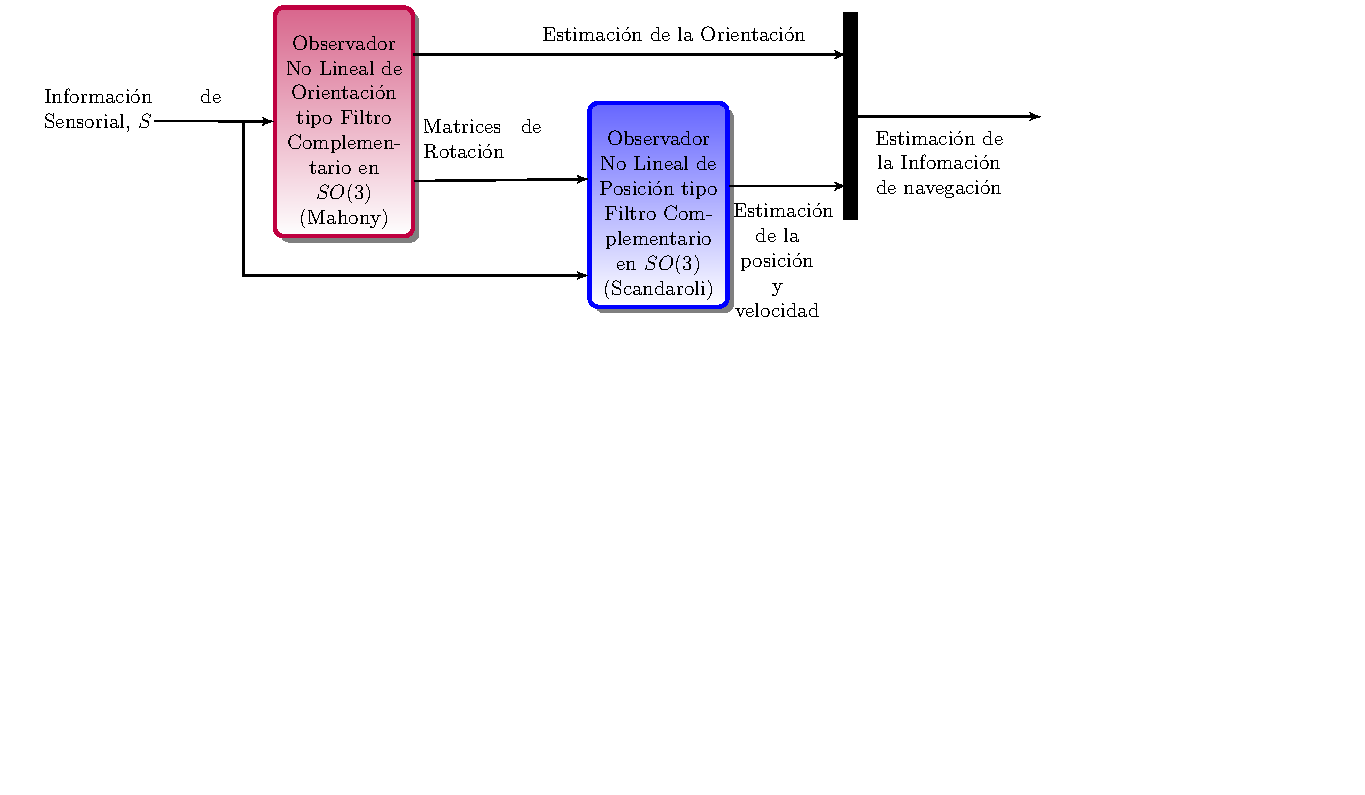
\includegraphics[scale=0.71,viewport=10 220 560 380,clip]{aam2.pdf}
%\caption{Condiciones cinemáticas de rotación sin deslizamiento de una rueda del robot.}
\caption{Esquema simplificado del algoritmo en observadores en cascada de Mahony-Scandaroli.}
\scriptsize{Fuente: Elaboración Propia}
\label{solucionMS_fig1}
\end{center}
\end{figure}
El algoritmo de navegación de Mahony-Scandaroli, puede ser esquematizado tal como se muestra en la Figura \ref{solucionMS_fig1}. En este esquema, el observador orientación toma parte de la medición de los sensores de navegación (elementos del conjunto de \emph{información sensorial disponible} $S$) para estimar:
\begin{itemize}
\item La orientación en términos de los ángulos de Euler.
\item La velocidad angular en $\marco{B}$
\item El error de estimación de la matriz de rotación $\tilde{R}$, definida como la transformación $\marco{E}\hookrightarrow\marco{B}$, donde $\marco{E}$ denota el marco referencial de estimación definido a través del error de la estimación de la orientación en $SO(3)$.
\item Y la matriz $\hat{R}$ para $\marco{E}\hookrightarrow\marco{A}$.
\end{itemize}
En cascada, el observador de posición tipo Filtro complementario en SO(3), toma el resto de las variables incluidas en $S$ junto con las matrices de transformación determinadas por el anterior algoritmo, para obtener la estimación de la posición y su derivada en $\marco{A}$. Finalmente, los dos grupos de variables estimadas por ambos observadores conforman la \emph{estimación de la información de navegación}, que puede ser denotada por el vector columna $X=[\hat{p}~\hat{v}~\hat{\Theta}~\hat{\Omega}]$, donde $\hat{p}$ es la estimación de la posición en $\marco{A}$, $\hat{v}$ es la estimación de la velocidad en $\marco{A}$, $\hat{\Theta}$ es la estimación de la orientación en términos los ángulos de Euler, y $\hat{\Omega}$ es la estimación de la velocidad angular en $\marco{B}$.
\subsubsection{Observador de orientación tipo filtro complementario en $SO(3)$.}
Específicamente, el trabajo de Mahony se concentra en la proposición de un algoritmo, para determinación de la orientación de un cuerpo rígido, en términos de la cinemática rotacional en el espacio ortogonal especial de tres dimensiones $SO(3)$. Ahí, se analizan dos observadores diferenciados en:
\begin{itemize}
\item \emph{El filtro complementario activo}.- que usa la medición de la matriz de rotación $R_y$ para proyectar la velocidad angular $\Omega_s$ al marco inercial, y resolver la estimación de la matriz de rotación $\hat{R}$ y el \emph{bias} de la velocidad angular $\hat{b}_\Omega$.
\item \emph{El filtro complementario pasivo}.- que usa $\hat{R}$ en realimentación, en vez de $R_y$ para proyectar la velocidad.
\end{itemize}
Dentro del enfoque de filtros complementarios, estos algoritmos fusionan dos entradas: la medición de la velocidad angular, y la medición de la orientación en términos de la matriz de rotación.\par
%%
Ahora bien, debido a que ambos algoritmos basan el desarrollo de sus ecuaciones en el análisis del modelo cinemático de la rotación en $SO(3)$, es oportuno definir tal cinemática. 
\subsubsection{Cinemática rotacional en $SO(3)$}
El concepto de Espacio Ortogonal Especial $SO(3)$, puede ser entendido a través del concepto de transformación de $\marco{B}\hookrightarrow\marco{A}$, denotada por la matriz de rotación en la ecuación \eqref{modelo_ecc1}. Esta matriz de transformación está caracterizada por dos propiedades fundamentales \bcite{Trola2009}:
\begin{enumerate}
\item Su determinante es \emph{unitaria positiva} para cualquier secuencia de rotación en los ángulos de Euler.
\item Y su inversa es igual a su transpuesta, otra vez, para cualquier secuencia de rotación en los ángulos de Euler. 
\end{enumerate}
Esta matriz establece la transformación de rotación de un elemento del espacio Euclídeo tridimensional, la cual mantiene la distancia del punto transformado respecto a un punto particular.
Específicamente, cuando además de mantener la distancia mantiene también la dirección, este tipo de rotación es denominada \emph{rotación propia}\footnote{A diferencia de las rotaciones impropias que invierten el orden de los puntos, y por lo tanto la rotación.}, y está caracterizada por la positividad de su determinante.
\begin{equation}
det(R)=1
\end{equation}
Donde $R$ es la matriz de rotación.\par
%%
Ahora, el conjunto total de transformaciones de rotación propias posibles establecidas dentro de los rangos de variación de los ángulos de Euler
\begin{gather*}
-\pi\leq(\phi,\theta,\psi)\leq\pi
\end{gather*}
Estructuran el llamado \emph{Espacio Ortogonal Especial de dimensión tres}, denotado $SO(3)$. Siendo este definido como un conjunto de matrices de transformación, denotadas genéricamente con $A$, que cumplen las dos propiedades características de la matriz de rotación, de esa manera el $SO(3)$ se define como:
$$SO(3)=\{\forall A \in \mathbb{R}^{3\times 3}/ A^T=A^{-1},det(A)=1\}$$
El álgebra de Lie asociada al $SO(3)$ se define como el conjunto de matrices anti-simétricas.
$$\mathfrak{so}(3)=\{\forall A \in \mathbb{R}^{n\times n}/ A=-A^T\}$$ 
Se define el operador de anti-simetría
\footnote{La matriz anti-simétrica permite fácilmente identificar el producto vectorial de dos vectores en $\mathbb{R}^3$, $a$ y $b$ tal que $$a\times b=a_\times b$$} $(\cdot)_\times:\mathbb{R}^3\rightarrow\mathfrak{so}(3)$, de forma tal que cualquier vector de tres dimensiones puede ser trasladado al algebra de Lie ortogonal especial de dimensión tres. Por ejemplo, sea: $$\left\{\Omega \in\mathbb{R}^3: \Omega=[\Omega_1~\Omega_2~\Omega_3]^T\right\}$$ Entonces
\begin{equation}
\Omega_\times=\begin{bmatrix}0&-\Omega_3&\Omega_2\\
\Omega_3&0&-\Omega_1\\
-\Omega_2&\Omega_1&0\end{bmatrix}
\end{equation}
%%
El operador inverso de $(\cdot)_\times$ se define como 
$$vex(\cdot):\mathfrak{so}(3)\rightarrow\mathbb{R}^3$$
Considerando lo anteriormente mencionado, la cinemática rotacional en $SO(3)$ puede ser entendida por el ritmo de cambio de la transformación de un elemento puntual fijo en el marco $\marco{B}$, y que rota con una velocidad angular $\Omega$ respecto al marco $\marco{A}$. Bajo estas condiciones es posible demostrar, a través de la equivalencia de la representación de la velocidad tangencial en términos del producto cruz de la velocidad angular con el vector de posición del elemento puntual, y la representación de la velocidad tangencial en términos la matriz de rotación, que la ecuación que representa la cinemática rotacional en $SO(3)$ está dada por:
%
%
%
%, donde, sin perder generalidad los orígenes de los marcos referenciales $\marco{A}$ y $\marco{B}$ coinciden, y además el marco $\marco{B}$ rota con una velocidad angular 
%(descrita por el vector $\vect{\Omega}$\footnote{Se adopta la notación de que un vector expresado como la combinación lineal de los vectores base de un marco de denota con letras negrillas, de esa forma, por ejemplo: un vector $v=[v^\mathcal{A}_1~v^\mathcal{A}_2~v^\mathcal{A}_3]^T$ en el marco referencial inercial $\marco{A}$ se denota como $\vect{v}=v^\mathcal{A}_1e_1^\mathcal{A}
%+v^\mathcal{A}_2e_2^\mathcal{A}
%+v^\mathcal{A}_3e_3^\mathcal{A}$.}) 
%respecto a $\marco{A}$.\par
%%%
%En estas condiciones el vector que describe el movimiento de elemento puntual denotado $\vect{r}(t)$, puede ser expresado por medio de un tensor, según la convención de signos de Einstein( Referencia \bcite{Einstein2}), en el marco $\marco{A}$ y el $\marco{B}$ como:
%\begin{equation}\label{modelo_ecc5}
%\vect{r}= r_i^\mathcal{B}e^\mathcal{B}_i(t)= r_j^s(t)e^s_j
%\end{equation}
%Siendo, $i$ y $j$ los sub-índices contravariantes (que varian entre uno y tres), $r_i^\mathcal{B}$ las componentes del vector $\vect{r}$ en el marco $\marco{B}$, $e^\mathcal{B}_i(t)$ los versores unitarios del marco referencial $\marco{B}$, $r_j^\mathcal{A}(t)$ las componentes del vector $\vect{r}$ en el marco $\marco{A}$, y $e^s_j$ los versores unitarios del marco $\marco{A}$. Se debe notar un contraste importante en las representaciones del vector $\vect{r}$, donde: la descripción del movimiento respecto de $\marco{B}$ muestra que el tensor $r_i$ tiene valores constantes y la base del marco se mueve con una velocidad angular instantánea $\vect{\Omega}$; al contrario del $\marco{A}$ donde la base es constante y el tensor tiene componentes que dependen del tiempo.\par
%%%
%Sin perder generalidad podemos decir que en $t=0$ los marcos están alineados es decir, $$ e_i^\mathcal{B}(0)=e_i^s~~~~r_i^s(0)=r_i^\mathcal{B}$$ Tomando en cuenta esto, $R’(t)$\footnote{La definición original define la transformación de $\marco{B}$ al $\marco{S}$, pero en este caso $R’$ denota la transformación inversa.} representa la transformación $$r(0)=r_j^\mathcal{B}e_j^s\rightarrow_{R’_{ji}}r(t)=r_I^se_i^s(t)$$ Entonces según la convención de Einstein $$r_i^s(t)=R’_{ij}(t)r_i^\mathcal{B}$$ Se deriva respecto del tiempo, y se tiene $$\dot{r}_i^s=\dot{R}’_{ij}r_j^\mathcal{B}=\dot{R}’_{ij}R’_{kj}r_k^s$$ Dado que $R’(t)\in SO(3)$, a partir de $R’R’^T=I_3$, 
%es fácil demostrar que el producto $\dot{R}’_{ij}R’_{kj}$ son los componentes de un tensor asimétrico, denotado por 
%$X_{ik}$. Entonces la velocidad se puede escribir como, \begin{equation}\vect{v}=e_i^\mathcal{B}X_{ik}r^\mathcal{B}_k.\end{equation} Ahora, como el único movimiento asociado con la velocidad angular se escribe al vector de velocidad como $$\vect{v}=\vect{\omega}\times\vect{r}$$ Que es igual al determinante y puede ser escrito en términos tensor asimétrico \begin{equation}\vect{v}=e_i^\mathcal{B}S(\omega)_{ik}r_k^\mathcal{B}.\end{equation}
%Y finalmente se tiene la ecuación diferencial que resume el comportamiento $R(t)$ en \eqref{modelo_ecc71}, retomando la notación original y usando el hecho de que $R’(t)=R^T(t)$.
\begin{equation}\label{modelo_ecc71}
\dot{R}=R\Omega_\times
\end{equation}
Donde $R$ es la matriz de rotación, y $\Omega_\times$ en la matriz del operador de anti-simetría aplicado la velocidad angular.
\subsubsection{Versión implementable del filtro complementario de Mahony}
Considerando la formulación de los dos observadores desarrollados por Mahony, su implementación requiere tener a disposición las señales correspondientes a la velocidad angular $\Omega_s$ y de la matriz de rotación $R_y$. En el caso de la velocidad angular es directamente obtenida utilizando un giroscopio. Ahora bien, en el caso de la matriz de rotación se debe tomar en cuenta algún método de reconstrucción a partir de información que encapsula el estado de orientación del cuerpo. Particularmente, Mahony utiliza la reconstrucción vectorial y re-formula estos observadores en términos de las mediciones vectoriales. La inclusión de esta reconstrucción vectorial en el esquema del filtro complementario pasivo, es definida por Mahony como \emph{filtro complementario explícito}.\par
%%
La reconstrucción vectorial es expresada en \begin{equation}\label{aam_ecc1}
R_y=\sum_{i=1}^n\sum_{j=i}^n(v_{0i}^T)(v_{0i})(v_{0j}^T)(v_{j})
\end{equation} Donde $v_j$ son los valores unitarios de las mediciones vectoriales, y $v_{0i}$ (ó $v_{0j}$) las direcciones unitarias conocidas de vectores medidos en $\marco{A}$, y $n$ el número de valores vectoriales disponibles, con $i$ y $j$ índices de la sumatoria.\par
%%
Entonces, Mahony define esta re-formulación en:
\begin{defin}\label{aam_def1}
El Filtro Complementario Explícito es el observador no lineal que determina la estimación de la orientación en $SO(3)$ ($\hat{R}$) y la estimación del \bias del giroscopio ($\hat{b}_{\Omega}$); resolviendo el par $\{\hat{R},b_{\Omega}\}$ en la siguientes ecuaciones diferenciales:
\begin{equation}\label{aam2}
\begin{array}{c}
\dot{\hat{R}}=\hat{R}S(\Omega_s-\hat{b}_\Omega+k_1\lambda)\\
\dot{\hat{b}}_{\Omega}=-k_2\lambda\\
\lambda=\sum_{i=1}^{n}k_iv_i\times\hat{v}_i
\end{array}
\end{equation}
Donde $v_j$ son los valores unitarios de las mediciones vectoriales y $\hat{v}_i$ son los valores unitarios de estimaciones de las mediciones vectoriales, establecidas por la proyección de los valores unitarios de los vectores conocidos $v_{0i}$ del marco $\marco{A}$ al marco $\marco{E}$ por la matriz estimada $\hat{R}$, y donde $k_1$ y $k_2$ son las constantes de diseño. Estas ecuaciones se resuelven en las condiciones iniciales $\hat{R}_0$ y $\hat{b}_{\Omega,0}$.
\end{defin}
El filtro complementario explícito guarda las propiedades de invulnerabilidad al ruido por utilizar la retroalimentación de la estimación de la matriz de rotación, en términos de medición directas de la IMU. Este observador es ideal para su implementación en plataformas de hardware embebidos. Además este filtro puede trabajar bien en el caso de que solo una dirección vectorial esté disponible.\par
%%
\begin{figure}
\begin{center}
\includegraphics[scale=0.71,viewport=0 30 550 340,clip]{aam_fig3.pdf}
\caption{Implementaciones del algoritmo de Mahony-Scandaroli.}
\scriptsize{Fuente: Modificado de [\cite{Mahony2008,Scandaro2011a}]}
\label{aam_fig2}
\end{center}
\end{figure}
%Por lo anteriormente señalado, el observador de orientación impermeable con la señales de los sensores disponibles para este trabajo, es el observador de orientación tipo filtro complementario $SO(3)$ en su versión explícita.\par
%%
\subsubsection{Observador de posición tipo filtro complementario en $SO(3)$.}
Por otro lado, [\cite{Scandaro2011}]: basado en el trabajo de Mahony expande la idea del uso del filtro complementario en $SO(3)$, para la observación de la posición, velocidad lineal y \emph{bias} de aceleración. Este autor, define la extensión del algoritmo poniendo en cascada un observador de posición tipo filtro complementario en las ecuaciones\footnote{El cual usa las matrices de transformación $\marco{E}\hookrightarrow\marco{A}$ y $\marco{E}\hookrightarrow\marco{A}$, resultado del anterior observador, además de la medición de la posición y de la aceleración.}.\par
%%
El observador de posición propuesto por Scadarolli basa su desarrollo en el análisis de estabilidad de Lyapunov, determinando tres constantes de actualización que garantizan la \emph{estabilidad asintótica en general} de tres variables: la velocidad lineal $\hat{v}$, el \emph{bias} de aceleración $\hat{b}_a$, y la posición . $\hat{p}$. Las constantes de actualización $\alpha_p$, $\alpha_v$ y $\alpha_a$ se expresan en las ecuaciones del observador de posición tipo filtro complementario en $SO(3)$ en:
\begin{equation}\label{problema_ecc5}
\begin{array}{c}
\dot{\hat{p}}=\hat{v}+\underbrace{k_3\tilde{p}}_{\alpha_p}\\
\dot{\hat{v}}=g^\mathcal{I}+\hat{R}(a_s-\hat{b_a})+\underbrace{k_4\tilde{p}}_{\alpha_v}\\
\dot{\hat{b}}_a=\underbrace{-k_5(I_3+\frac{1}{k_5}S(\Omega_s-\tilde{b}_\omega))\hat{R}^T\tilde{p}}_{\alpha_a}
\end{array}
\end{equation}
Donde $\tilde{p}$ es el error de estimación en la posición, y $k_3$ a $k_5$ son las constantes de diseño de este observador.\par
Estas constantes de actualización establecen una estructura típica del filtro complementario, con la medición de la aceleración $a_s$ como la señal de ruido de alta frecuencia y la medición de posición $p_y$ como la señal de ruido de baja frecuencia. 
\subsubsection{Estructura del algoritmo de navegación de Mahony-Scandaroli.}
En resumen, el enfoque original del algoritmo de observadores en cascada de Mahony-Scandaroli, resuelve la determinación de la información de navegación en tres niveles de procesamiento:
a) la reconstrucción vectorial de la matriz de rotación $R_y$ usando la medición de un acelerómetro $a_s$ y un magnetómetro $m_s$\footnote{El desarrollo teórico y práctico de Mahony en [\cite{Mahony2008}] demuestra que no es absolutamente necesario incluir ambas mediciones. Y si el caso fuese de que alguna de las señales es demasiado ruidosa se puede prescindir de la misma.}; b) la determinación de la estimación de la velocidad angular $\hat{\omega}$, la estimación de la orientación en términos de los ángulos de Euler $\hat{\Theta}$, y la estimación de la matriz de rotación $\hat{R}$ con su respectivo error $\tilde{R}$\footnote{Definida como $\tilde{R}=R_y\hat{R}^T$}, los que se determinan usando las señales de la reconstrucción vectorial y la medición de un giroscopio $\Omega_s$; c) la determinación de la estimación de la posición $\hat{p}$, y la velocidad lineal $\hat{v}$ a partir de las anteriores salidas, es decir $\tilde{R}$ y $\hat{R}$, junto con la medición de posición $p_y$ y la aceleración $a_s$. Este procedimiento está definido en el pseudo código \ref{aam_alg1}, al igual que en el diagrama de bloques de la Figura \ref{aam_fig2}.
\begin{algorithm}[ht]
\caption{Algoritmo de observadores tipo filtro complementario en $SO(3)$ de Mahony-Scandaroli.}\scriptsize
\label{aam_alg1}
\begin{algorithmic}
\State\textbf{1. Reconstrucción vectorial}
\begin{gather*}
\hat{v}_{0a}=\frac{g_0}{|g_0|}\\
\hat{v}_{0m}=\frac{m_0}{|m_0|}\\
\hat{v}_{a}=\frac{a_s}{|a_s|}\\
\hat{v}_{m}=\frac{m_s}{|m_s|}\\
R_y=k_a^2v_{0a}v^T_a+k_ak_mv_{0a}v^T_{0a}v_{0m}
v^T_m+k_m^2v_{0m}v^T_m
\end{gather*}
\State\textbf{2. Observador de Orientación}
\begin{gather*}
\dot{\hat{R}}=\hat{R}S(\Omega_s-\hat{b}_{\omega}+\alpha_R(R_y,\hat{R}))\\
\dot{\hat{b}}_\omega=\alpha_\omega(R_y,\hat{R})\\
\hat{\Omega}=\Omega_s-\hat{b}_{\omega}\\
\hat{\Theta}=f_1(\hat{R})
\end{gather*}
\State\textbf{3. Observador de Posición.}
\begin{gather*}
\dot{\hat{p}}=\hat{v}+\alpha_p(p_y,\hat{p})\\
\dot{\hat{v}}=g^\mathcal{I}+\hat{R}(a_s-\hat{b_a})\alpha_v(p_y,\hat{p})\\
\dot{\hat{b_a}}=\alpha_a(\hat{\Omega},p_y,\hat{p},\hat{R})
\end{gather*}
\end{algorithmic}
\end{algorithm}\par
En la etapa de \emph{reconstrucción vectorial}, se utilizan las mediciones del acelerómetro y del magnetómetro, $a_s$ y $m_s$, para calcular los valores unitarios $v_m$ y $v_a$, dividiendo estas medidas entre sus magnitudes. Con estos valores, y con $v_{0a}$ y $v_{0m}$, valores teóricos unitarios del vector gravitacional ($g_0$) y del vector del campo magnético terrestre ($m_0$), se determina la reconstrucción vectorial de la rotación: $R_y$.\par
Después, en la etapa \emph{observador de orientación} se solucionan las ecuaciones diferenciales del observador para determinar $\hat{R}$ y $\hat{b}_\Omega$ (estimaciones de la matriz de rotación y del \emph{bias} de medición del giroscopio) evaluando las variables denominadas constantes de actualización: $\alpha_R$ y $\alpha_\omega$. Con el valor de \bias del giroscopio se puede determinar la estimación de la velocidad angular $\hat{\Omega}$ como la diferencia de: la medición de la velocidad angular ($\Omega_s$) y el \bias del giroscopio ($\hat{b_\Omega}$). Y por último, se calcula la estimación de la orientación en términos de los ángulos de Euler ($\hat{\Theta}$) evaluando $f_1()$\footnote{Esta función hace la transformación de la matriz de rotación a los ángulos de Euler (ver \bcite{Zhong2002})}, definida a continuación:
\begin{equation}\label{FuncionInversaEuler}
f_1=\left\{
\begin{array}{l}
\phi=-arctag(R_{2,1}/R_{1,1})\\
\theta=-arcsin(R_{1,3})\\
\psi=-arctag(R_{3,2}/R_{3,3})
\end{array}\right.
\end{equation}
Donde $R_{2,1}$, $R_{1,1}$, $R_{1,3}$, $R_{3,3}$ y $R_{3,2}$, son los elementos fila-columna\footnote{Es decir, que el primer sub-índice corresponde al número de fila y el segundo sub-índice corresponde al número de columna.} de la matriz R (ver ecuación \eqref{modelo_ecc1}).\par
%%
En la última etapa se soluciona las ecuaciones diferenciales para $\hat{p}$, $\hat{v}$ y $\hat{b}_a$, de manera similar, evaluando las constantes de actualización; que son función de la medición de la posición $p_y$, la estimación de la posición $\hat{p}$, la estimación de la velocidad angular $\hat{\Omega}$ y/o la estimación de la matriz de rotación $\hat{R}$.\par
%%
\subsection{Pruebas de efectividad del algoritmo de navegación de Mahony y Scandaroli.}
En los trabajos de Mahony y Scandaroli se desarrollan diferentes pruebas que permiten ver la efectividad de la técnica que se plantea. En general, existen tres tipos de experimentos en donde se prueba la efectividad del algoritmo. En la Figura \ref{aam_fig2} se muestra tres ilustraciones que representan a cada uno de ellos:
\begin{itemize}
\item En el primer experimento se hace un análisis homográfico de un objeto de referencia para determinar la matriz de rotación y la posición. Se usa una IMU para determinar la velocidad angular y la aceleración. 
\item En el segundo experimento se usan ciertos sensores angulares de un brazo robótico, programado para mover una IMU, en la determinación de la matriz de rotación, y para el caso de la implementación de la versión explícita del filtro complementario de Mahony, se usa una medición artificial del vector de campo magnético con los valores de dichas mediciones angulares.
\item En el tercer experimento, se implementa el filtro complementario explícito usando solamente las señales de una IMU instalada en un VTOL MAV HoverEye de \emph{Bertin Technologies}.
\end{itemize} 
Independientemente de la forma en que se implemente, el algoritmo de Mahony-Scandaroli necesita la medición de la aceleración, de la velocidad angular, la posición y de la matriz de rotación.\par
%%
Debido a que no existe realmente un sensor que sea capaz de medir este último parámetro, el algoritmo define la reconstrucción de la matriz de rotación en la función de Lyapunov. En estas condiciones la presición de la estimación de la información de navegación depende del punto de estabilidad. Cuando el movimiento es constante, no existe mayor problema y la convergencia puede ser absoluta. Sin embargo, debido a que en un recorrido la orientación es un término en constante cambio, es posible que el valor encontrado no minimice el error. En ese entendido, la reconstrucción vectorial es un método sub-óptimo, el cual puede reducir la eficiencia de la estimación de la información de navegación.\par 
%%%%%%%%%%%%%%%%%%%%%%%%%%
%%%%%%%%%%%%%%%%%%%%%%%%%%
%%%%%%%%%%%%%%%%%%%%%%%%%%
%%%%%%%%%%%%%%%%%%%%%%%%%%
%%%%%%%%%%%%%%%%%%%%%%%%%%
\section{Reconstrucción Óptima de la matriz de rotación.}\label{Propuesta}
%%%%%%%%%%%%%%%%%%%%%%%%%%
%%%%%%%%%%%%%%%%%%%%%%%%%%
%%%%%%%%%%%%%%%%%%%%%%%%%%
%%%%%%%%%%%%%%%%%%%%%%%%%%
%%%%%%%%%%%%%%%%%%%%%%%%%%
Como señala Mahony, la principal desventaja en la formulación de los filtros complementarios pasivo y directo es la sensibilidad a la matriz de entrada $R_y$. Esta matriz es usada en el mapeo de la medición de la velocidad angular al marco inercial $\marco{A}$, y por esta razón, la determinación de esta matriz juega un papel central en el desempeño final del sistema.\par
%%
Considerando esto, el problema de mejorar la reconstrucción de la matriz de rotación es el punto focal del presente trabajo y representa su principal aporte. Para ello, se buscará solucionar de manera óptima el problema planteado en [\cite{Mahony2008}], el cual indica que: a partir de la medición de cantidades vectoriales conocidas respecto a $\marco{B}$, la matriz de rotación puede ser determinada en el argumento que minimiza la función de coste definida en:
\begin{equation}\label{chap2:DefincionRoptima}
R^*=\arg~\min_{R}\left\{\sum_i|v_{0,i}-Rv_{m,i}|^2\right\}
\end{equation}
Esta ecuación significa que la matriz de rotación óptima $R^*$ minimiza la función de coste compuesta por la suma de los cuadrados de los módulos de la diferencia de: los valores de las mediciones vectoriales rotadas al marco inercial (R$v_{m,i}$), respecto a los valores teóricos conocidos de dichas cantidades vectoriales ($v_{0,i}$)\footnote{Donde los sub-índices corresponden a las distintos valores vectoriales medibles.}
\subsection{Problema de la determinación de la matriz de rotación}
Como ya se mencionó en la anterior sección, el movimiento rotacional puede ser modelado en la derivada de la matriz de rotación $\dot{R}$ en el espacio ortogonal especial. En otras palabras, conociendo el comportamiento dinámico de $R$, es posible entender el movimiento rotacional. Esto también es válido para el caso inverso, es decir, que conociendo las variables que describen el movimiento se puede determinar el valor exacto de $R$. Lamentablemente, es imposible conocer de manera directa estas las variables (que describen el movimiento), y en su lugar, estas son determinadas en la medición de la inclinación en un campo vectorial conservativo constante, buscando empatar el modelo supuesto de rotación del cuerpo (el cómo se cree que se mueve el cuerpo) con el modelo de medición vectorial (como se mueve su entorno\footnote{El entorno visible, desde el punto de medición vectorial, constituye un campo vectorial conservativo.} respecto del cuerpo\footnote{Esto dado que un observador fijo al cuerpo (en el marco $\marco{B}$) observaría que el campo vectorial rota alrededor suyo.}). En la búsqueda de la determinación de tal modelo es importante entender el porqué y el cómo rota un cuerpo rígido.
\par
%% 
Como es natural, cuando un cuerpo rígido es sometido a fuerzas distantes de su centro de masa tiende a girar alrededor de este último. El efecto rotacional de estas fuerzas sobre este cuerpo es encapsulado en el concepto de torque; el cual se define como el producto vectorial entre el vector posición del punto donde se aplica la fuerza y la componente perpendicular de dicha fuerza a este vector. A partir de ello, se puede decir que la rotación es la consecuencia o el efecto directo de la incidencia de los torques en un cuerpo.\par
%% 
En este caso, el proceso de rotación -del cual se pretende extraer la determinación óptima de la matriz de rotación- considera la observación de la rotación de un cuerpo rígido en respuesta a una entrada de torques desconocidos. Donde, los efectos directos de estas entradas (torques) desde el punto de vista de una caja negra son:
\begin{enumerate}
\item El cambio dinámico de la variable de orientación, que en términos de los ángulos de Euler se denota $\Theta$.
\item El incremento o decremento de la velocidad angular respecto al marco referencial fijo al cuerpo, denotada $\Omega$. \end{enumerate}
%En este punto, dado que el modelo de rotación está completamente determinado por las variables de movimiento rotacional, es decir, por la orientación en $\Theta$ y la velocidad angular del cuerpo en $\Omega$, la matriz de rotación estaría de igual manera determinada. %Y como ya se mencionó, en la práctica la determinación exacta de estos valores no es posible.
\par
Entonces, en estos términos, el reto propuesto para la elaboración del algoritmo de reconstrucción de los estados que determinan la evolución de la matriz de rotación considera que: la medición de estos valores no es posible, y en su lugar son determinadas indirectamente, en la inclinación de vectores conocidos respecto al marco $\marco{B}$.\par
%%
\begin{figure}[t]
\begin{center}
\includegraphics[scale=1,viewport=10 30 400 170,clip]{ObsOptimo_fig7.pdf}
\caption{Esquema para la reconstrucción de la matriz de rotación usando la medición del vector gravitacional.}
\label{ObsOptimo_fig1}
\end{center}
\end{figure}
Dicho esto, la solución que se sigue en este trabajo plantea la reconstrucción de la matriz de rotación a partir de la medición del vector gravitacional, tal como se esquematiza en la Figura \ref{ObsOptimo_fig1}. En donde, las proyecciones de las componentes del vector gravitacional (denotado por $\vect{g}_0$) respecto al marco referencial fijo al cuerpo \textcolor{red}{$\marco{B}$} ( representado en la Figura \ref{ObsOptimo_fig1} con las flechas rojas) permiten obtener la orientación del \textsl{cuerpo rígido}; y con ello, la matriz de rotación que transforma la representación del vector de gravedad en $\marco{B}$ a su representación en $\marco{A}$.\par
%%
De esa manera, el problema se traslada en el hecho de que: la aplicación de esta metodología requiere la definición de un modelo matemático que emule el comportamiento de la rotación, que es consecuencia directa de la aplicación de los torques incidentes en el cuerpo. De ahí, la dificultad radica en que estos torques son desconocidos, por lo tanto el modelo debe ser definido de tal modo que no dependa de estas entradas.\par
\subsection{Determinación de la matriz de rotación a partir del modelo de medición del vector gravitacional en cuaterniones.}
\begin{figure} [t]
\begin{center}
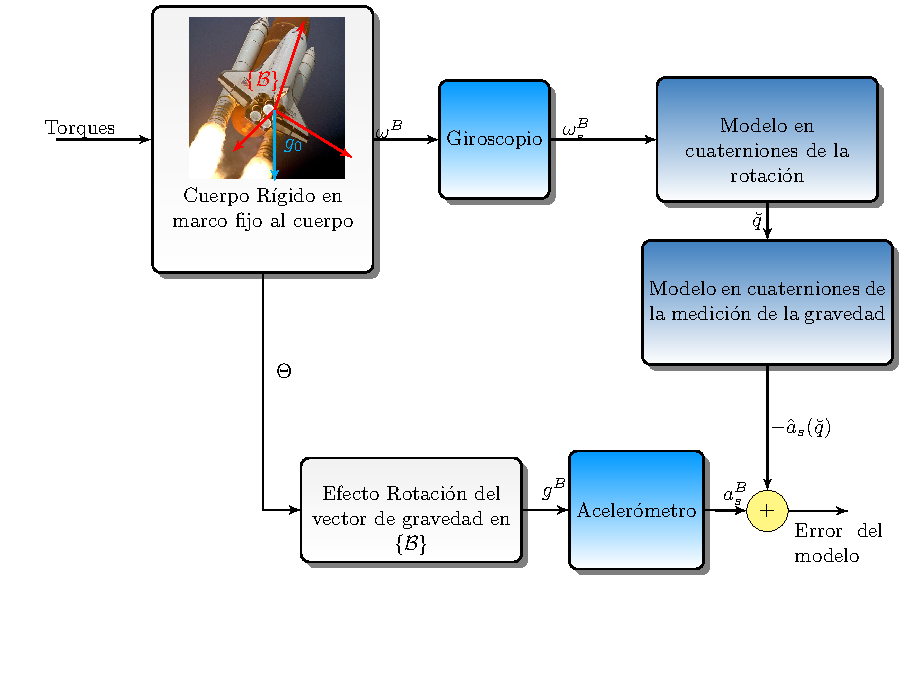
\includegraphics[scale=0.850,viewport=20 50 430 330,clip]{ObsOptimo_fig3.pdf}
\caption{Caracterización del error del modelo de medición.}
\label{ObsOptimo_fig2}
\end{center}
\end{figure}
%%
El esquema desde donde obtiene la orientación a partir de la medición vectorial de la gravedad -considerando la indeterminación de los torques efectivos en cuerpo- incorpora el modelo cinemático de la rotación en cuaterniones. Este esquema está representado en la Figura \ref{ObsOptimo_fig2}, donde la caja negra del proceso de rotación excitado por los \emph{torques} desconocidos, produce dos señales que representan la orientación y su velocidad de cambio, es decir en las salidas $\Theta$ y $\Omega$, respectivamente. Estos parámetros son medidos:
\begin{enumerate} 
\item La velocidad angular por un giroscopio, obteniendo $\Omega_s$.
\item La orientación $\Theta$, de manera indirecta, midiendo la inclinación del vector gravitacional respecto al marco fijo al cuerpo $\marco{B}$, usando un acelerómetro.
\end{enumerate}
La medición de la velocidad angular es la entrada con la que el modelo cinemático en cuaterniones\footnote{Los cuaterniones son una generalización de los números complejos en cuatro dimensiones, introducidas por Hamilton en 1853. El lector interesado en un desarrollo histórico de la teoría en cuaterniones, ver referencia [\cite{Warden1976}]} determina la evolución de la rotación en términos de un cuaternión unitario (denotado $\breve{q}$). Aquí, dado que este cuaternión está definido en las rotaciones de los ángulos de Euler, según la fórmula de Rodrigues
\footnote{La teoría en cuaterniones tiene varias aplicaciones en interpretación de fenómenos y leyes físicas, por su parte en sistemas de computación tiene aplicaciones en animación, y simuladores de vuelo, por mencionar algunos pocos. Por su parte, la modelación de la rotación en términos de cuaterniones otorga grandes ventajas computacionales, que permiten un cómputo inmediato de las rotaciones, además de evitar puntos de singularidad. La rotación usando cuaterniones es propuesta por el matemático francés Rodrigues, en la denominada fórmula de Rodrigues [\cite{Kuipers1999}].} (ver \bcite{Altmann1986}) permite hacer la representación de la medición vectorial de la gravedad ($\hat{a}_s$) en el marco $\marco{B}$, a partir del valor conocido de la gravedad $[0,0,g_0]^T$ en $\marco{A}$. A partir de ello, la señal proveniente del acelerómetro $a_s$ (excitada por la efecto de la rotación del vector de la gravedad en $\marco{B}$) se define el error de la evolución del modelo.
\par
%%
De esa manera, el cuaternión unitario, denotado por $\breve{q}=q_0+q_1i+q_2j+q_3k$ en $\mathbb{Q}:\mathbb{R}\times\mathbb{C}^3$, contiene las rotaciones necesarias para transformar un vector de $\marco{B}$ al $\marco{A}$, y sus componentes son \bcite{Cai2011}:
\begin{gather}\label{modelo_ecc3}
\begin{array}{c}
q_0=\cos\frac{\phi}{2}\cos\frac{\theta}{2}\cos\frac{\psi}{2} + \sin\frac{\phi}{2}\sin\frac{\theta}{2}\sin\frac{\psi}{2}\\
q_1=\sin\frac{\phi}{2}\cos\frac{\theta}{2}\cos\frac{\psi}{2} + \cos\frac{\phi}{2}\sin\frac{\theta}{2}\sin\frac{\psi}{2}\\
q_2=\cos\frac{\phi}{2}\sin\frac{\theta}{2}\cos\frac{\psi}{2} + \sin\frac{\phi}{2}\cos\frac{\theta}{2}\sin\frac{\psi}{2}\\
q_3=\cos\frac{\phi}{2}\cos\frac{\theta}{2}\sin\frac{\psi}{2} + \sin\frac{\phi}{2}\sin\frac{\theta}{2}\cos\frac{\psi}{2}
\end{array}
\end{gather}
%%
La derivada de $\breve{q}$ compone el modelo cinemático de la rotación como un producto de cuaterniones \footnote{Denotada por el símbolo $\otimes$} de la velocidad angular en $\mathbb{Q}$\footnote{Definida como un cuaternión puro, en donde la parte real es cero, y las componentes están repartidas en $i$, $j$ y $k$, para la velocidad angular en los ejes $x$, $y$ y $z$, respectivamente} ($\breve{\Omega}$) y el cuaternión unitario ($\breve{q}$) como sigue\footnote{ Para una descripción específica y deducción de las ecuaciones de cuaterniones usadas ver [\cite{Kuipers1999}].}:
\begin{equation}
\dot{\breve{q}}=\frac{1}{2}\breve{q}\otimes\breve{\Omega}
\end{equation}
Escrita matricialmente esta es \bcite{Zhong2002}:
\begin{equation}\label{modelo_ecc7}
\begin{bmatrix}\dot{q}_0\\\dot{q}_1\\\dot{q}_2\\\dot{q}_3\\ \end{bmatrix}= \frac{1}{2}\begin{bmatrix} 0&-p&-q&-r\\ p&0&r&-q\\ q&-r&0&p&\\ r& q&-p&0\\ \end{bmatrix} 
\begin{bmatrix} q_0\\q_1\\q_2\\q_3\\ \end{bmatrix}= \frac{1}{2}\begin{bmatrix} 0&-\Omega^T\\ \Omega&\Omega_\times \end{bmatrix}\breve{q}
\end{equation}
%%
Finalmente el modelo cinemático de la rotación que incorpora el \emph{bias} de medición de la velocidad angular, se define en la ecuación: 
\begin{gather}\label{chap2:ModeloProceso}
\begin{array}{c}
\dot{q}=\frac{1}{2}S(\Omega_s-b_{\Omega})q\\
\dot{b}_\Omega=0
\end{array}
\end{gather}
%%
Seguidamente, el modelo de la medición de la gravedad usando el cuaternión unitario se expresa en \bcite{Sola2012}:
\begin{equation}\label{chap2:ModeloMedicion}
\hat{a}_s=\bar{\breve{q}}\otimes\breve{g_0}\otimes\breve{q}=Rg_0=g_0\begin{bmatrix}2(q_1q_3-q_oq_2)\\2(q_2q_3+q_0q_1)\\q_0^2-q_1^2-q_2^2-q_3^2\end{bmatrix}
\end{equation}
En resumen, el proceso que teóricamente determinaría la matriz de rotación usando el modelo en cuaterniores, asume que es posible determinar la orientación en el tiempo $T$: ajustando los parámetros del modelo en cuaterniones en función a un historial de mediciones exactas del vector gravitacional $a_s$; de forma tal que se busca la evolución de $\breve{q}$ que gira al vector gravitacional exactamente en el valor de $\hat{a}_s(T)$, reduciendo así el \emph{error del modelo} a cero. Entonces, a partir de las componentes de $\breve{q}$ los elementos de la matriz de rotación serían cabalmente determinadas en \bcite{Sola2012}:
\begin{equation}\label{modelo_ecc4}
R^T=\begin{bmatrix} q^2_0+q^2_1-q^2_2-q^2_3&2(q_1q_2+q_0q_3)&2(q_1q_3-q_0q_2)\\ 2(q_1q_2-q_0q_3)&q^2_0-q^2_1+q^2_2-q^2_3&2(q_2q_3+q_0q_1)\\ 2(q_1q_3+q_0q_2)&2(q_2q_3+q_0q_1)&q^2_0-q^2_1-q^2_2+q^2_3\\ \end{bmatrix}
\end{equation} 
Lamentablemente, dado que en la práctica el proceso de medición incorpora una enorme cantidad de lagunas, impediría encontrar el valor exacto (y seguramente, ni siquiera el óptimo) de la matriz de rotación usando esta metodología. Por consiguiente, parece oportuno emplear ciertas correcciones que puedan eliminar coherentemente las imperfecciones, y así, depurar el valor de $\breve{q}$ buscando reducir el \emph{Error del Modelo} aproximadamente a cero de la mejor manera posible.\par
%%
Este concepto va muy de la mano con la definición de óptimización. Y puede ser interpretado como la búsqueda óptima de los estados del cuaternión unitario y el \emph{bias} del giroscopio que reducen el costo de desviación de la medición de la gravedad de \emph{manera óptima} o de \emph{la mejor manera}. Esto define el problema de determinación óptima de la matriz de rotación usando un modelo en cuaterniones.
\subsection{Correcciones iterativas óptimas al modelo de medición vectorial}
El problema de ajuste anteriormente mencionado tiene cierta relación con el esquema de estimación de los estados ocultos de la Teoría de Grafos en un diagrama de Markov de primer orden: donde, los estados ocultos, que conforman una serie de tiempo estocástica, se relacionan con la medición en una probabilidad de transición acumulativa que depende de las anteriores mediciones.\par
%%
\begin{figure}[t]
\includegraphics[width=\textwidth]{hiddenMarkov.jpg}
\caption{Ejemplo de un diagrama de Markov de primer orden para un sistema dinámico estocástico de tercer orden.} \scriptsize{Las relaciones establecen dos niveles: el primero corresponde al espacio de estados ocultos, que muestra la evolución de los estados en tiempo los cuales no son accesibles; el segundo nivel es el nivel observable constituido por las salidas medibles del sistema. Fuente: [\cite{Perrin2003}]}
\label{recons_fig1}
\end{figure}
De manera análoga, el problema de la determinación del cuaternión que ajusta la medición del vector de gravedad se puede plantear de la siguiente manera \bcite{Merwe2004}: \begin{quote} Imaginemos que tenemos un conjunto de datos pasados de la medición $y_k=\{y_i\}_{i\in\{k_0,...,k_f\}}$ en tiempo discreto en el intervalo $i\in\{k_0,...,k_f\}$, y queremos determinar el estado oculto $x_{k_f}$, sabiendo que cada elemento de $y_k$ está relacionado por una función discreta del conjunto de elementos $x_k=\{x_i\}_{i\in\{k_0,...,k_f-1\}}$.\end{quote}
%%
En este caso la evolución de tiempo discreto de los estados ocultos se denota en
\begin{equation}
\label{chap2:ecc1}
x_{k+1}=f_k(x_k,u_k)
\end{equation} 
Donde $x_k=[\breve{q},b_\Omega]$ son los estados ocultos compuestos por el cuaternión unitario y el \emph{bias} de la velocidad angular, $u_k$ las entradas al sistema. \par Estos estados se relacionan con la medición vectorial de la siguiente manera:
\begin{equation}
\label{chap2:ecc10}
y_{k}=h_k(x_k)
\end{equation} 
Siendo $h_k$ una función no lineal.\par El problema se mantiene en la búsqueda del estimado de los estados ocultos $\hat{x}_{k+1}$ haciendo correcciones sucesivas en la incertidumbre del modelo $w_k$ modelo que estima el comportamiento (donde, $f^o_k$ es el modelo incierto del proceso) en:
\begin{equation}
\label{chap2:ecc11}
\hat{x}_{k+1}=f^o_k(\hat{x}_k,u_k)+w_k
\end{equation}
\par
Midiendo el error en la incertidumbre del modelo de medición $v_k$, en:
\begin{equation}
\label{chap2:ecc4}
v_k=y_k-\underbrace{h_k(\hat{x}_k)}_{\hat{y}_k}
\end{equation}
Donde $\hat{y}_k$ corresponde a la ecuación \ref{chap2:ecc10} evaluada en el punto de estimación actual.\par
Desde el punto de vista de optimización, este mismo problema se ve como la búsqueda del conjunto de datos de la incertidumbre del modelo $$w_k=\{w_{k_0}...w_{k_f}\}$$ que reducen los errores de la evolución de la estimación $$\tilde{x}_k=\hat{x}_k-x_k$$ (desde la condición inicial $\tilde{x}_{k_0}=\hat{x}_{k_0}-x_{k_0}$) y de medición $$\tilde{y}_k=v_k=y_k-\hat{y}_k$$ minimizando la función de costo:
\begin{equation}\label{recons_ecc1}\min_{w_k}\left\{g_0(\tilde{x}_k,\tilde{y}_0)+ \sum_{i=1}^{N}\Xi_k(w_k,\tilde{y}_k) \right\}\end{equation}
Donde la función de coste depende de la acumulación de los errores de medición (plasmados en la incertidumbre de medición) $\tilde{y}_k=h(\hat{x}_k)$ y del error de estimación $\tilde{x}=\hat{x}_k-x_k$, ambos errores englobados en la función $\Xi_k(w_k,\tilde{y}_k)$; junto con los errores iniciales conocidos $g_0(\tilde{x}_k,\tilde{y}_0)$. Donde, $\Xi$ y $g_0$ son funciones matriciales definidas positivas.\par
%%
Una alternativa de solución a este problema es usar Programación Dinámica (PD) en la versión lineal: del modelo del proceso en $x_k$ y del modelo de la medición; la cuales se definen en los Jacobianos de primer orden en las series de Taylor de $f_k$ y $h_k$, alrededor de un punto fijo.\par
%%
La PD es una rama derivada de la teoría de programación no lineal [\cite{Avriel2003}], la cual segmenta un problema complejo en pequeños sub-problemas, de tal forma que solucionando uno de ellos, es posible aplicar el mismo concepto para solucionar iterativamente los otros. Esto se puede realizar, bajo el sustento del Principio de Optimización de Bellman que dice:
\begin{quote}
El conjunto de entradas $\{u^*_k\}$ entre $\{k_0,...,k_f\}$ se determina encontrando las expresiones que calculan el óptimo entre $k_f-1$ y $k_f$, y generalizando las mismas para encontrar todos los elementos de $\{u^*_k\}$ [\cite{Lewis2012}].
\end{quote} 
A partir de ello podemos encontrar, conceptualmente la corrección del tiempo actual $k_f=k$ considerando el historial de mediciones encapsuladas en la información de $k-1$ hacia atrás.\par
%%
Entonces, se procede linealizando las ecuaciones del modelo del proceso y de medición en un punto fijo propio para la linealización, en:
\begin{gather}
x_{k+1}=F_0x_k+B_0u_k\\
y_{k}=H_0x_k\label{chap2:MedicionLineal}
\end{gather}
Donde los $F_0$, $B_0$ y $H_0$ son los Jacobianos de $f_k$ para $x_k$, $u_k$ y $h_k$ para $x_k$, respectivamente, en $x_0$ y $u_0$. Entonces la dinámica del observador y su error se determinan en las ecuaciones:
\begin{gather}
\hat{x}_{k+1}=F_0\hat{x}_k+B_0u_k\\
\hat{y}_{k}=H_0\hat{x}_k\\
\tilde{x}_{k+1}=F_0\tilde{x}_k\\
\tilde{y}_{k}=H_0\tilde{x}_k
\end{gather}
De ahí el problema de observador óptimo se define en:
\begin{defin}[Problema Observador Óptimo Lineal]\label{problemaobsoptlineal}
Sea un sistema lineal discreto descrito en:
\begin{equation}
\label{filtro_ecc3}
x_{k+1}=Fx_k+Bu_k
\end{equation} 
Donde, $F$ es la matriz del proceso, $B$ es la matriz de entradas, $x_k$ son los estados ocultos y $u_k$ las entradas al sistema; las que se relacionan con las variables de salida de tal forma que:
\begin{equation}
\label{filtro_ecc4}
y_{k}=Hx_k
\end{equation} 
Donde $H$ es la matriz de salida, y $y_k$ es la salida medible (observable) del sistema.
Entonces, el problema de optimización se define como el encontrar el set de datos $\hat{x}_k=\{\hat{x}_{k_0}...\hat{x}_{k_f}\}$, de manera que se cumpla $$\hat{x}_k=\arg\min_{x_k}\left\{(\tilde{x}_0+H\tilde{y}_0)^T
P(\tilde{x}_0+H\tilde{y}_0)+ \sum_{i=1}^{N} \begin{bmatrix}\tilde{x}_k\\\tilde{y}_k\end{bmatrix}^T
\begin{bmatrix}Q&0\\0&R\end{bmatrix} \begin{bmatrix}\tilde{x}_k\\\tilde{y}_k\end{bmatrix} \right\}$$
Donde la función de coste depende de la acumulación de los errores de medición (plasmados en la incertidumbre de medición) $\tilde{y}_k=h(\hat{x}_k)$ y del error de estimación $\tilde{x}=\hat{x}_k-x_k$; junto con los errores iniciales conocidos $g_0(\tilde{x}_k,\tilde{y}_0)$. Además $P$, $Q$ y $R$, son positivas, denominadas matrices de peso.
\end{defin}
Ahora ahí, aplicamos el principio de Bellman en el intervalo de tiempo $[k,N]$ cuando $k\in\{0,...,N\}$, invertiendo el orden la sumatoria con $k=N-k$, entonces la función coste mínima $J^*_k(x_k)$ para este subintérvalo $\{k,...,(N=k+1)\}$ se puede expresar de manera sencilla en (usando la notación de la ecuación \eqref{recons_ecc1}):
\begin{gather}
J_k(x_k)=\min_{u_k} \left\{\sum_{i=k}^{kf=k+1}\Xi_i(x_k,u_k)+g_{kf=k+1})\right\}\label{filtro_ecc33}
\end{gather}
Con la inversión del orden de la sumatoria, la ecuación dinámica del error se escribe:
$$F\tilde{x}_{k+1}+w_k=\tilde{x}_k$$
$$\tilde{x}_{k+1}=F^{-1}\tilde{x}_k-\underbrace{F^{-1}w_k}_{\tilde{w}_k}$$
%En estas condiciones, es equivalente modificar la función de coste , por las variables de incertidumbre $\tilde{w}_k$ por $\tilde{x}_k$, y $\tilde{y}_k$ por $v_k$. Haciendo esto, la función de coste...
De ahí la función de coste mínima se puede expresar entonces como:
$$\hat{x}_k=\arg\min_{x_k}\left\{\begin{bmatrix}\tilde{x}_k\\\tilde{y}_k\end{bmatrix}^T
\begin{bmatrix}F^{-T}QF^{-1}+P&CP\\PH^T&R+H^TPH\end{bmatrix} \begin{bmatrix}\tilde{x}_k\\\tilde{y}_k\end{bmatrix} \right\}$$
De ahí se usa el lema del complemento de Schur en 
$\tilde{x}_k$ y se tiene las siguientes ecuaciones:
\begin{gather}
w_{k}=-\underbrace{P_kH_k^T(R+H_kP_kH_k^T)}_K\tilde{y}_k\\
w_k^TF^{-T}P_kA^{-1}w_k=w_k^T(F^{-T}QF^{-1}+P_k-KH_kP_k)w_k
\end{gather}
Lo que establece el estimador de los estados ocultos en:
\begin{equation}\label{chap2:ObservadorLineal}
\hat{x}_{k+1}=F\hat{x}_k+Bu_{k}+K(y_k-H\hat{x}_k)
\end{equation}
Donde $\hat{x}_k$ es la estimación de los estados ocultos, $y_k$ es la medición vectorial de la gravedad. \par
%%
El diseño considera las matrices $H_0$ y $F_0$ como los Jacobianos de $f_k$ y $h_k$, en un punto de linealización fijo; y evalúa la Ecuación Discreta de Riccati de forma iterativa con $P_{k=0}=P_0$, en:
\begin{equation}\label{filtro_ecc10}P_{k+1}=Q+F_k(P_k-KH_kP_k)F_k^T\end{equation}
Junto con la ganancia del Observador. \begin{equation}\label{filtro_ecc11}
K=P_kH_k^T(R+H_kP_kH_k^T)^{-1}
\end{equation}
A partir de esto, es posible establecer un algoritmo adaptable en cada punto de la estimación, que calcula una ganancia del observador $K$ y los Jacobianos $H_0$ y $F_0$\footnote{Denotando estas matrices como $H_k$ y $F_k$, respectivamente.} en cada $k$ \par
Este algoritmo está relacionado con el Filtro de Kalman Extendido, con la diferencia de que las matrices $Q$ y $R$ no son asociadas a las propiedades aleatorias de las incertidumbres del modelo y de la medición, sino al análisis de la respuesta temporal de los errores de estados en el dual del controlador óptimo. Este es el algoritmo denotado como el Observador Óptimo tipo Filtro de Kalman Extendido (EKF, ver pseudo-código \ref{alg1}) .\par
\begin{algorithm}[h!]
\caption{Algoritmo del Observador Óptimo tipo de EKF}
\label{alg1}
\begin{algorithmic}
\Require $P_0$
\State \textbf{Calcula Jacobianos:} $F_k$ y $H_k$
\State\textbf{Actualiza la matriz de Peso}: 
$$P_k=Q+F_k(P_{k-1}-KH_{k}P_{k-1})F_k^T$$
\State \textbf{Determina la matriz de ganancia:}$$K=P_kH_k^T(R+H_kP_kH_k^T)$$
\State\textbf{Se calcula la estimación:}
\State $\hat{x}_{k+1} = F_k\hat{\vect{x}}_k+K(a_s-h_k(q_k))$
\end{algorithmic}
\end{algorithm}
%\subsection{Filtro de Kalman como un Observador Óptimo}
%\par
%%% 
%El filtro de Kalman tiene sus orígenes en la Teoría de Filtrado Estocástico, e inicia con los trabajos de [\cite{Wiener1942}] y [\cite{Kolmogorov1941}]. Es celebrado como uno de los enfoques más exitosos en este tipo de filtros, y tiene una extensa lista de aplicaciones en diferentes campos, como en biología, navegación, economía. Inicialmente el filtro de Kalman se desarrolla para estimación óptima de los estados de un \emph{sistema lineal}, pero se amplia sobre el mismo concepto para la estimación en sistemas no lineales en el Extended Kalman Filter (EKF).\par
%%%
%Dado que el concepto esencial del filtro de Kalman es la estimación de los estados ocultos de un sistema en forma \textit{óptima}. Este es capaz de determinar la $\breve{q}$ como el estado oculto el cual ajusta el problema de óptimo. En otras palabras, encuentra $\breve{q}$ que calcula $R^*$, cuadrando el modelo de rotación con el modelo de medición.\par
%%%
%El filtro de Kalman puede ser derivado como un observador óptimo de tiempo discreto, el cual soluciona la determinación de los estados en \emph{problema del observador óptimo}, estableciendo el problema del Filtro de Kalman determinístico:
\subsection{Filtro de Kalman dual del Control Óptimo}\label{dualidad}
Un observador de estado es el sistema que calcula el valor de las variables que describen el comportamiento de un sistema, en base a la medición parcial y ruidosa de sus salidas y entradas [\cite{Buchi2010,Korovin2009}]. Por otro lado, el controlador es el sistema que en base a medición parcial y ruidosa calcula las entradas $u_k$ que hacen que el sistema este en ciertas condiciones finales, y reduce el error hacia el punto de estabilidad deseado. Estas dos definiciones matizan cierta semejanza que será desarrollada adelante.\par
%%
En teoría de control la dualidad entre problema de control óptimo y el observador óptimo no es tema nuevo. En el artículo original de Kalman [\cite{Kalman1960}] se termina resaltando la importancia y resume una serie de ecuaciones de equivalencia. Inclusive existe literatura actual que trata este tema e.g. [\cite{Yan2012}].\par
%%
De manera general, en el control óptimo se busca reducir el estado de un sistema lo más rápido posible en un intervalo de tiempo $\{t0,...t_f\}$, y al mismo tiempo se busca no hacer demasiado esfuerzo de control (medido en la magnitud de la entrada de control $u(t)$). De esa manera, el regulador óptimo establece el problema de la determinación la entrada de control óptima $u(t)$ en el intervalo $\{t0,...t_f\}$, que minimiza una función de costo similar a la ecuación \ref{recons_ecc1}, [\cite{Goodwin2000}].\par
En el caso de un sistema lineal discreto invariante en el tiempo denotado en:
\begin{equation}\label{chap2:ecc2}
x_{k+1}=F^{Control}x_k+B^{Control}u_k
\end{equation}
Donde $F^{Control}$ es la matriz del proceso y $B^{Control}$ es la matriz del entradas, ambas asociadas al controlador óptimo.\par
El controlador resultante -denominado \emph{Regulador Óptimo Cuadrático} \footnote{Linear Quadratic Regulator} (LQR)- resuelve $u_k$ reduciendo la evolución de $x_k$ en la función de coste denotada como:
\begin{equation}\label{chap2:ecc12}
{u}_k=\arg\min_{u_k}\left\{x_0^T
Px_0+ \sum_{i=1}^{N} \begin{bmatrix}{x}_k\\{u}_k\end{bmatrix}^T
\begin{bmatrix}Q&0\\0&R\end{bmatrix}^T \begin{bmatrix}{x}_k\\{u}_k\end{bmatrix} \right\}
\end{equation}
De manera similar, la solución del Estimador Óptimo Lineal considera el estimador lineal de la ecuación \eqref{chap2:ObservadorLineal}, el cual busca reducir el error de estimación $\tilde{x}_k$ lo más rápido posible en un intérvalo discreto de tiempo $\{k_0,....,k_f\}$, reduciendo además la incertidumbre de medición $\tilde{y}_k=v_k$.\par
%%
Bajo estas condiciones, reemplazando la ecuación (2.28) en la ecuación del estimador lineal (2.34) se obtienen las equivalencias de dualidad del \emph{Control Óptimo} con el \textsl{Observador Óptimo}:
\begin{equation}\label{filtro_ecc7}
\tilde{x}_{k+1}^T=\tilde{x}_{k}^T(F_k^T +H_k^TK^T)
\end{equation}
Que es equivalente al reemplazo de la ley del control del LQR en la ecuación del Control Óptimo reemplazando la ley de control en la ecuación \eqref{chap2:ecc2}
\begin{equation}\label{filtro_ecc8}
\vect{x}_{k+1}=(F_k^{Control}+B^{Control}_kK)\vect{x}_{k}
\end{equation}
De ahí las equivalencias son fácilmente determinadas estableciendo :
\begin{equation}\label{chap2:EcuacionesDual}
F_k^{Control}=F_k^T ~~~~B^{Control}_k=H_k^T
\end{equation}
Entonces, a partir de ello podemos decir que solucionando el LQR en el sistema lineal invariante en el tiempo:
\begin{equation}\label{chap2:ecc13}
x_{k+1}=F^Tx_k+H^Tu_k
\end{equation}
Se resuelve en realidad el dual del observador óptimo. En cuyo caso, la matriz de ganancia $K^{LQR}$, equivale a la transpuesta de la ganancia $K$ del observador óptimo.
\begin{equation}
K^{LQR}=K^T
\end{equation}
%%%%%%%%%%%%%%%%%%%%%%%%%%%%%
%%%%%%%%%%%%%%%%%%%%%%%%%%%%%
%%%%%%%%%%%%%%%%%%%%%%%%%%%%%
\section{Análisis de respuesta temporal en Filtros Complementario en $SO(3)$}\label{obs_acp1}
La complejidad de los fenómenos involucrados en el problema de navegación conforma sistemas bastante complejos, los cuales pueden escapar del enfoque de los observadores lineales. Consecuentemente, es necesario proponer un observador que sea capaz de conservar la no linealidad natural del sistema y de capturar aquellos detalles que se pierden durante el proceso de linealización. Por esta razón, los \emph{observadores de estado no lineales} son ideales para aplicaciones en las que el sistema tiene fuertes acoples no lineales.\par
%%
Existen varios enfoques de diseño de este tipo de observadores; dentro de los cuales se encuentra los observadores no lineales tipo filtro complementario en $SO(3)$. Esta variedad de observadores en su definición plantean los factores de corrección al modelo cinemático en variables (denominadas \emph{constantes de actualización}) extraídas del análisis de estabilidad en el sentido de Lyapunov\par
%%
A continuación se describe basado en el trabajo \bcite{Scandaro2011} un método para diseñar los parámetros de esta variedad de filtros, donde se definen las condiciones para encontrar los autovalores de manera independiente en las cinco direcciones de estimación, las cuales son: el \emph{bias} del giroscopio $\hat{b}_{\Omega}$, la matriz de rotación $\hat{R}$, la posición $\hat{p}$, la velocidad lineal $\hat{v}$ y el \emph{bias} del acelerómetro $\hat{b}_a$. 
\subsection{Análisis de respuesta temporal en el filtro complementario Orientación en $SO(3)$.}\label{sec_epsilon}
El observador de orientación tipo filtro complementario $SO(3)$ esta denotado por las siguientes ecuaciones:
\begin{equation}\label{FConSO3_ecc1}
\dot{\hat{R}}=\hat{R}(\Omega_y-b_\Omega+k_1\omega)_\times,~~~\dot{\hat{b}}_\Omega=-k_2\omega
\end{equation}
Donde $\hat{R}$ y $\hat{b}_\Omega$ son las estimaciones: de la matriz de rotación y del \emph{bias} del giroscopio, respectivamente, junto con $\omega$, el término de corrección definido por Mahony, como la proyección del espacio del error de la estimación de la matriz de rotación a un espacio tangencial al $SO(3)$, y el par $k_1$ y $k_2$ son las constates de diseño. \par
\begin{figure}
\center
\includegraphics{analisisFC_fig1.pdf}
\caption{Proceso de estimación del Observador de Orientación tipo filtro complementario en $SO(3)$.}
\scriptsize{Fuente: Elaboración Propia.}
\label{analisisFC_fig1}
\end{figure} 
Este observador está definido como una variación al modelo cinemático de la rotación (ver ecuación \eqref{modelo_ecc71}) al cual se le aplican correcciones sistemáticas en dos variables, denominadas \emph{variables de actualización}; donde $\alpha_R$ es la corrección al modelo de rotación en $SO(3)$ y $\alpha_\Omega$ es la corrección al modelo del comportamiento del \bias del giroscopio, las cuales se sintetizan en el término de corrección $\omega$, extraído del análisis de estabilidad de Lyapunov en la búsqueda de una solución a la función candidata de Lyapunov \footnote{Como ya se menciona, en los artículos \bcite{Mahony2005,Mahony2006} se propone la variable de actualización como la proyección del error a un espacio tangencial al $SO(3)$.}:
\begin{equation}
\lypf=\frac{1}{2}tr(I_3-\tilde{R})+\frac{1}{2k_2}|\tilde{b}_\Omega|^2
\end{equation}
Donde $\tilde{R}$ es error de estimación de la matriz de rotación, $\tilde{b}_\Omega$ el error de estimación del \emph{bias} del giroscopio, e $I_3$ es la matriz identidad de tres dimensiones; y su solución se establece como:
\begin{equation}\label{FConSO3_ecc2}
\dot{\lypf}=-k_1|\lucia|^2=-k_1|\omega|^2
\end{equation}
Donde $P_a$ es la proyección antisimétrica\footnote{Definida como: $P_a(\cdot) =\frac{(\cdot)-(\cdot)^T}{2}$.} aplicada al error de observación de la matriz de rotación, y $vex(\cdot)$ en el inverso al operador $(\cdot)_\times$.\par
De esa manera $\alpha_\Omega$, $\alpha_R$ son definidos en:
\begin{equation}\label{obs_ecc2}
\alpha_R=k_1\hat{R}^Tvex(P_a(\tilde{R})):=k_1\omega, ~ \alpha_\Omega=-k_2\hat{R}^Tvex(P_a(\tilde{R})):=-k_2\omega
\end{equation}
Con el término de corrección:
\begin{equation}
\omega=\lucia
\end{equation}.\par
Donde el error de estimación de la matriz de rotación se establece como:
\begin{equation}
\tilde{R}=R_y\hat{R}
\end{equation}
De esa manera, el proceso de estimación en el observador no lineal de orientación tipo filtro complementario en $SO(3)$, establece tres niveles de procesamiento:
\begin{itemize}
\item La etapa de medición, empleando métodos directos como la medición de velocidad angular con un giroscopio, o indirectos como la reconstrucción vectorial de la matriz de rotación
\item La etapa de corrección, en la actualización del término de corrección que es función de los errores de estimación.
\item Y la etapa de estimación, usando en modelo de la cinemática de rotación corregido por las variables de actualización (ver Figura \ref{analisisFC_fig1}).
\end{itemize}
Se puede entender el esquema del filtro complementario en $SO(3)$ como el equivalente de las operaciones del espacio Euclídeo en el espacio ortogonal especial. Este análisis, realizado por Mahony, es representado en la Figura \ref{FConSO3_fig2}: donde
\begin{figure}[t]
\center
\includegraphics[width=\textwidth]{FConSO3_fig2.jpg}
\caption{Diagrama de bloques de la forma general del filtro complementario en el $SO(3)$}
\scriptsize{Fuente: \bcite{Mahony2008}}
\label{FConSO3_fig2}
\end{figure}
la operación $\hat{R}^T$ es equivalente a la multiplicación por -1 en la etapa de retroalimentación del filtro complementario en frecuencia; la $\hat{R}R_y$ equivalente a la resta de la medición y la estimación; los operadores $P_a(\tilde{R})$ y $(R\Omega)_\times$ proyectan el error de la estimación de la matriz de rotación y la velocidad angular en un espacio tangente al espacio ortogonal $SO(3)$, las cuales son integradas en el equivalente en $\mathfrak{so}(3)$ de una cinemática de primer orden\footnote{Donde una cinemática de primer orden puede ser entendida como la ecuación en el tiempo de un filtro de primer orden denotado por: $\dot{y}+C_1y=u$, siendo $y$ la salida, $C_1$ una constante en $\mathbb{R}$ y $u$ la entrada a tal filtro.} . \par
Ahora bien, con respeto a las contantes de diseño ($k_1$ y $k_2$) estas son determinadas por medio del análisis de respuesta transitoria sobre las versiones linealizadas de las ecuaciones \eqref{FConSO3_ecc1} (alrededor del punto $(I_3,0)$ que corresponde a las condiciones nulas de la dinámica del error). El proceso de linealización inicia con los siguientes cambios de variable: 
\begin{equation*}
\tilde{R}=I_3+(\tilde{\Theta})_\times
\end{equation*}
Donde $\tilde{\Theta}$ son los errores de la estimación de los ángulos de Euler. Además se incluye:
\begin{equation*}
\epsilon=R\tilde{b}_\omega
\end{equation*}
Con su derivada:
\begin{equation*}
\dot{\epsilon}=\dot{R}\tilde{b}_\omega+k_2 \lucia
\end{equation*}
De ahí se define la dinámica lineal simplificada del error de estimación en este observador como.
\begin{equation}\label{obs_ecc4}
\begin{bmatrix}\dot{\tilde{\Theta}}\\\dot{\epsilon}\end{bmatrix}=
\begin{bmatrix}-k_1I_3&-I_3\\k_2I_3&0_3\end{bmatrix}
\begin{bmatrix}\tilde{\Theta}\\\epsilon\end{bmatrix}
\end{equation}
Esta última ecuación establece tres polinomios -con autovalores $\lambda_1=-3/\tau_1$ $\lambda_2=-3/\tau_2$- característicos de la forma:
\begin{equation}
s^2+k_1s+k_2=0
\end{equation}
De ahí es fácil demostrar que las constantes de diseño asociadas a este a un comportamiento temporal de las variables estimas se calculan como:
\begin{equation}\label{obs_ecc10}
k_1=3\frac{\tau_1+\tau_2}{\tau_1\tau_2}~~k_2=9\frac{1}{\tau_1\tau_2}
\end{equation}
Después, realizando una serie de transformaciones entre las realizaciones equivalentes de la Ecuación \eqref{obs_ecc4} se puede demostrar que las salidas de estimación obedecen a las siguientes ecuaciones exponenciales, donde $\tilde{\Theta}_i$ y $\epsilon_i$ son una de las componentes de los cambios de variables ya definidos; y $f_{12}$ con $f_{21}$ son funciones exponenciales complejas:
\begin{equation}
\begin{array}{c}\label{EcuacionesExponenciales1}
\tilde{\Theta}_i=\tilde{\Theta}_i(0)e^{\lambda_1t}+\frac{f_{12}}{\lambda_1-\lambda_2}\epsilon_i(0)+\frac{\lambda_2f_{12}}{\lambda_1-\lambda_2}\tilde{\Theta}_i(0)\\
\epsilon_i=\epsilon_i(0)e^{\lambda_2t}+\frac{\lambda_2f_{21}}{\lambda_1-\lambda_2}\epsilon_i(0)+\frac{\lambda_1\lambda_2f_{21}}{\lambda_1-\lambda_2}\tilde{\Theta}_i(0)
\end{array}
\end{equation}
Esto demuestra el carácter exponencial decreciente en $(I_3,0)$ para autovalores distintos y reales.\par
%%
En esta última ecuación es fácil deducir que la relación $\lambda_1>>\lambda_2$ equivalente a $\tau_2>>\tau_1$ garantiza un rápido decremento de los elementos residuo en los estados de los errores en los ángulos de Euler $\tilde{\Theta}$, pero si $\lambda_2$ es demasiado pequeña la dinámica de $\epsilon$ será lenta.\par
%%
Es importante resaltar, que el observador está desarrollado para cualquier cuerpo. Además, necesita de dos entradas: la velocidad angular que proviene de un giroscopio; y la matriz de rotación que proviene de la reconstrucción óptima ($R^*$) a partir de $\breve{q}_k$,o proviene de la reconstrucción vectorial de la matriz de rotación\footnote{Que se define el filtro complementario Explícito.} ($R_y$). Ahora, si bien este observador es estable, su confiabilidad está estrechamente relacionada con la calidad de sus entradas.\par
\subsection{Análisis de respuesta transitoria para el filtro complementario de posición.}
El anterior observador permite estimar la orientación y la velocidad angular. Sin embargo, para obtener una estimación completa de la cinemática de un cuerpo rígido de seis grados de libertad esta estimación no es suficiente. En ese sentido [\cite{Scandaro2011}] propone el observado de posición en cascada con el filtro complementario de orientación. \par
%%
El observador de posición de [\cite{Scandaro2011}] está definido para la estimación de la posición $\hat{p}$, la estimación de la velocidad $\hat{v}$ y la del \emph{bias} de aceleración $\hat{b}_{a}$ en:
\begin{equation}\label{obs_ecc5}
\begin{array}{c}
\dot{\hat{p}}=\hat{v}+k_3\tilde{p}\\
\dot{\hat{v}}=g^\mathcal{A}_0+\hat{R}(a_s-\hat{b_a})+k_4\tilde{p}\\
\dot{\hat{b}}_a=-k_5(I_3+\frac{1}{k_3}S(\Omega_s-\tilde{b}_\omega))\hat{R}^T\tilde{p}
\end{array}
\end{equation}
Donde $\tilde{p}$ es el error de estimación en la posición, $k_3$, $k_4$ y $k_5$ son las constantes de diseño.\par
%%
De la misma manera que el observador de orientación, este observador está constituido en una modificación del modelo de cinemática lineal y del \bias del acelerómetro, al cual se le hacen correcciones sistemáticas proporcionales al error de estimación de la posición. \par
%%
Este observador puede ser esquematizado en tres etapas similares al esquema del observador de orientación (ver Figura \ref{FConSO3_fig4}) donde:
\begin{itemize}
\item La primera etapa corresponde a la recopilación de la información, correspondiente a la medición de la velocidad angular, la medición de la aceleración, la estimación del bias del giroscopio y la estimación de la matriz de rotación\footnote{Proveniente del observador de orientación tipo filtro complementario en $SO(3)$.}.
\item La segunda etapa corresponde al cálculo de las constantes de actualización $\alpha_p$ para el modelo cinemático de la posición, $\alpha_v$ para el modelo cinemático de la velocidad lineal, y $\alpha_a$ para el modelo del comportamiento del \bias de aceleración.
\item Y en la última etapa corresponde a la evaluación del modelo cinemático del movimiento lineal corregido por las constantes de actualización (el cual deriva en las ecuaciones \eqref{obs_ecc5}) para el estimado del resto de las componentes de la información de navegación.
\end{itemize}
\begin{figure}
\center
\includegraphics{analisisFC_fig4.pdf}
\caption{Esquema del funcionamiento del filtro complementario de posición.}
\scriptsize{Fuente: Elaboración Propia.}
\label{FConSO3_fig4}
\end{figure}
Los errores de estimación $\tilde{p}$, $\tilde{v}$ y $\tilde{b}_a$, para la posición, velocidad y \bias de aceleración se expresan como:
\begin{equation}
\begin{array}{c}
\tilde{p}=p-\hat{p}\\
\tilde{v}=v-\hat{v}\\
\tilde{b}_a=b_a-\hat{b}_a
\end{array}
\end{equation}
Y su dinámica.
\begin{equation}\label{obs_ecc60}
\begin{array}{c}
\dot{\tilde{p}}=\tilde{v}-k_3\tilde{p}\\
\dot{\tilde{v}}=-R\tilde{b}_a-k_4\tilde{p}\\
\dot{\tilde{b}}_a=k_5(I_3+\frac{1}{k_3}S(\Omega))R^T\tilde{p}
\end{array}
\end{equation}
Estas ecuaciones permiten establecer a Scandaroli, definir las condiciones de estabilidad del Observador de Posición en $SO(3)$, bajo la condicionante del análisis previo en el observador de orientación. En ese entendido, el observador completo, que fusiona ambos observadores define en el punto de estabilidad $(\tilde{R},\tilde{b}_{\Omega},\tilde{p},\tilde{v},\tilde{b}_a)\rightarrow(I_3,0,0,0,0)$, de tal forma que la derivada de función de Lyapunov
$$\mathcal{V}=\frac{1}{2}(k_4-\frac{k_5}{k_3})|\tilde{p}|^2+\frac{1}{2}|\tilde{v}|^2+\frac{k_3}{2k_5}|\tilde{\gamma}|^2$$ 
Es decreciente bajo las condiciones en que la ecuación \eqref{FConSO3_ecc2} de la derivada de la función de Lyapunov del filtro complementario de orientación, también es decreciente. Donde la variable $\gamma$ equivale a:
$$\gamma=R\tilde{b}_a-\frac{k_5}{k_3}\tilde{p}$$
Lo que nos permite establecer el decrecimiento de $\mathcal{V}$ en función al error de la estimación de la posición:
$$\dot{\mathcal{V}}=-k_3(k_4-\frac{k_5}{k_3})|\tilde{p}|^2$$
%%
Debido a que se garantiza la estabilidad exponencial para los errores de estimación de movimiento lineal ($\tilde{p}$, $\tilde{v}$ y $\tilde{b}_a$), podemos linealizar alrededor del punto (0,0,0), donde $\epsilon=R\tilde{b}_a$ expresa la dinámica del error del \bias de aceleración respecto al marco inercial, de tal manera que se establece el siguiente sistema lineal.
\begin{equation}\label{obs_ecc8}
\begin{bmatrix}\dot{\tilde{p}}\\\dot{\tilde{v}}\\\dot{\tilde{\epsilon}}\end{bmatrix}=
\begin{bmatrix}-k_3&1&0\\-k_4&0&-1\\k_5&0&0
\end{bmatrix}\begin{bmatrix}\tilde{p}\\\tilde{v}\\\tilde{\epsilon}\end{bmatrix}
\end{equation}
Cuyo polinomio característico es $$\lambda^3+k_3\lambda^2+k_4\lambda +k_5=0$$ Si sus autovalores establecen $$\lambda_3=-\frac{3}{\tau_3}~\lambda_4=-\frac{3}{\tau_4}~\lambda_5=-\frac{3}{\tau_5}$$ Entonces 
\begin{equation}\label{obs_ecc12}
k_3=3\frac{\tau_3\tau_4+\tau_3\tau_5+\tau_4\tau_5}{\tau_3\tau_4\tau_5}~~~k_4=9\frac{\tau_3+\tau_4+\tau_5}{\tau_3\tau_4\tau_5}~~~k_5=-\frac{27}{\tau_3\tau_4\tau_5}
\end{equation}
La matriz de relación formada por los autovectores establece la siguiente relación.\begin{equation}\label{obs_ecc6}
\begin{bmatrix}x_3\\x_4\\x_5\end{bmatrix}=
\begin{bmatrix}-\lambda_4\lambda_5&\lambda_4+\lambda_5&1\\
-\lambda_3\lambda_5&\lambda_3+\lambda_5&1\\
-\lambda_3\lambda_4&\lambda_3+\lambda_4&1\\
\end{bmatrix}\begin{bmatrix}\tilde{p}\\\tilde{v}\\\tilde{\epsilon}\end{bmatrix}
\end{equation}
Las soluciones espacio de estados en su representación modal es de la forma.
\begin{equation}\label{obs_ecc7}
\begin{array}{c}
x_1(t)=x_1(0)e^{\lambda_1t}\\
x_2(t)=x_2(0)e^{\lambda_2t}\\
x_3(t)=x_3(0)e^{\lambda_3t}
\end{array}
\end{equation}
Usando \eqref{obs_ecc6} se pueden expresar las condiciones iniciales de la representación modal en función de las condiciones iniciales de los errores de estimación, esa relación se reemplaza en \eqref{obs_ecc7}, volviendo a llevar esto al lado derecho de \eqref{obs_ecc6}, con un álgebra un poco engorrosa se encuentran la evolución temporal de los errores de estimación como:
\begin{equation}\label{obs_ecc9}
\begin{array}{c}
\tilde{p}_i=e^{\lambda_3t}\tilde{p}_i(0)+\frac{f_1}{(\lambda_4-\lambda_5)(\lambda_3-\lambda_5)}\tilde{v}_i(0)+\frac{f_2}{(\lambda_4-\lambda_5)(\lambda_3-\lambda_5)}\epsilon_i(0)\\
\tilde{v}_i=e^{\lambda_4t}\tilde{v}_i(0)+\frac{f_3}{(\lambda_4-\lambda_5)(\lambda_3-\lambda_5)}\tilde{p}_i(0)+\frac{f_4}{(\lambda_4-\lambda_5)(\lambda_3-\lambda_5)}\epsilon_i(0)\\
\epsilon_i=e^{\lambda_5t}\epsilon_i(0)+\frac{f_5}{(\lambda_4-\lambda_5)(\lambda_3-\lambda_5)}\tilde{p}_i(0)+\frac{f_6}{(\lambda_4-\lambda_5)(\lambda_3-\lambda_5)}\tilde{v}_i(0)
\end{array}
\end{equation}
Donde $f_1$, $f_2$, $f_3$, $f_4$, $f_5$ y $f_6$ son funciones complejas exponenciales, que la misma manera que en la ecuación \eqref{EcuacionesExponenciales1}, se deduce que $\tau_5>>\tau_4,\tau_3$, garantiza una influencia despreciable de tales términos
%%%%%%%%%%%%%%%%%%%%%%%%%%
%%%%%%%%%%%%%%%%%%%%%%%%%%
%%%%%%%%%%%%%%%%%%%%%%%%%%
\newpage
\section{Fundamentos en navegación GPS}\label{FundamentosEnNavegacionGPS}
Compuestos por una constelación de 24 satélites orbitando nuestra atmósfera, el sistema de geo-posicionamiento global (GPS) ha traído un revolución en la forma de desplazarse de las personas en el siglo XXI. La miniaturización de los dispositivos receptores GPS, permitieron su inclusión en teléfonos celulares inteligentes, automóviles e incluso animales, y junto con plataformas como Google-Maps, Waze, Sygic o AndNav permiten a millones de usuarios desplazarse en ciudades, carreteras, parques nacionales, e incluso en alta mar con poco o nada de conocimiento de navegación, y sistemas como el Tagg Pet o LoJack permiten rastrear mascotas perdidas o automóviles robados.\par
En sistemas de navegación se usan diferentes medios para realizar la medición de la posición, tales como cámaras, radares. etc. Sin embargo cuando la aplicación requiere el monitoreo en áreas vastas y a campo abierto, la mejor opción es usar un GPS. En este acápite se desarrolla la teoría fundamental de la navegación usando GPS. Para ello, este acápite se divide en: a) Funcionamiento de un GPS b) Sistema geódico coordenado c) Mensajes NMEA-MKT.
\subsection{Funcionamiento de un GPS}\label{gps_sec1}
Un GPS es un sistema de localización en el cual se envían códigos de Ruido Pseudo-Aleatorio (PRN\footnote{\emph{Pseudo Random Noise Code} en inglés}) con pulsaciones generadas por un reloj atómico montado un satélite, esta señal baja hacia la tierra y es recepcionada por un usuario, de tal forma que el módulo en tierra calcula la distancia entre la antena del receptor y el emisor basado en el tiempo de viaje del código. \par
%%
De forma más detallada el sistema funciona de la siguiente manera, cada satélite envía un PRN modulado por una secuencia de datos binarios (únicos en cada satélite) denominado en inglés Coarse/Adquisition (C/A). Posteriormente, este código viaja a casi la velocidad de la luz hasta el receptor en tierra, en forma de una señal de radiofrecuencia BPSK en una sinusoide portadora\footnote{La portadora para usuarios civiles es la banda L1 de 1575.42MHz.}. Y después el módulo GPS en la tierra, en primer lugar calcula el estado del código, después conociendo dicho estado hace la resta tiempo en que se recibió el mensaje menos el periodo del código y el tiempo de deducción de estado, para finalmente en base a la comparación con los otros satélites se obtienen los tiempos de viaje\footnote{Tiempo que tarda el código PRN en llegar al receptor en tierra.} para cada satélite. El tiempo de viaje se multiplica por la velocidad de la luz calculando la distancia del cada satélite al punto de recepción del módulo.\par
%%
Con la captura de tres distancias se puede calcular fácilmente por la intersección de tres esferas el punto en cuestión, ya que se conoce exactamente la posición de cada satélite en el momento en que empiezan a mandar el código C/A. Sin embargo, dado que el reloj del receptor no está exactamente sincronizado con los relojes montados en la constelación de satélites, se tiene una incógnita denominada error de sincronización. Considerando esto es necesario contar con una ecuación más y así determinar la cuarta variable, dicho esto es imprescindible tener como mínimo el enlace con por lo menos cuatro satélites. \par
\subsubsection{Organización de la constelación de satélites del GPS.}
Los satélites están organizados en órbitas circulares alrededor de la tierra, en cada órbita están dispuestos cuatro satélites separados aproximadamente 30, 105, 120, y 105 grados. Los seis planos orbitales tienen una inclinación de 55º respecto del plano del Ecuador, separados 60º de ascensión derecha del nodo de ascendencia. Cada satélite orbita con un periodo igual a mitad de un día sideral, es decir 11 horas y 58 minutos, a una distancia promedio de 26000km del centro de la tierra.\par
%% 
Esta disposición permite tener en visión al menos a 6 satélites a la vista en cualquier punto del planeta \bcite{Zogg2002}. 
\subsubsection{Fuentes de error en el GPS}
\begin{table}
\begin{center}
\caption{Desviaciones Estándar $1-\sigma$ de la medición de la posición con el sistema de posicionamiento global (GPS) }

\begin{tabular}{c|c} \hline
\textbf{Nombre del Parámetro}&\textbf{Rango de Error Equivalente de Usuario [m]}\\ \hline
%--------------------------------------------------------------------->
Limitaciones del C/A &$0.5$\\ 
Efectos de la Ionosfera& $4$\\ 
Error de efemérides& $2.1$\\
Error del reloj del satélite& $2.1$\\
Distorsión multipath& $1.4$\\
Efectos de la Troposfera& $0.7$\\ \hline
UERE${}^*$=$\sigma_R$& $5.3$\\ \hline
\end{tabular}
\label{fundamentosGPS_tb3}

\end{center}
\scriptsize{*El acrónimo anglosajón UERE significa Rango equivalente de Error de Usuario (User Equivalent Range Error). Además el acrónimo C/A significa Coarse/Adquisition o Adquisición/Tosca\\
Fuente: \bcite{Bradford2001}}
m\end{table}
En el sistema GPS pequeños errores de transmisión y decodificación pueden significar varios cientos de metros de error, así que los sistemas de transmisión están calibrados con mucho detalle.\par
%%
Como en todo sistema de transmisión inalámbrico la cantidad de errores se limita al medio y la calidad de los módulos electrónicos. Específicamente en el GPS las principales fuentes de error (compiladas en la tabla \ref{fundamentosGPS_tb3} como desviaciones estándar en metros) pueden ser divididas en:
\begin{enumerate}
\item Las limitaciones de la capacidad de la técnica de codificación, delimitadas por la longitud del código y velocidad de transmisión.
\item Los retardos de ionosfera en la señal causados por los rebotes de la onda transmitida por el satélite en la partículas que conforman la ionosfera terrestre.
\item Lo errores en los cálculos de la información relacionada con la orbitación de los satélites, considerando las fórmulas de Kepler y lo efectos de atracción de la luna y el sol. Donde la información orbita es enviada cada cuatro o cinco horas por cada satélite en un archivo ASCII denominado \emph{Efemérides}.
\item Los errores de los factores de corrección para el cálculo de los errores de sincronización entre los relojes de los satélites y el del receptor.
\item Los retardos causados por el cambio de las características eléctricas del medio protagonizadas por la capa de vapores y cristales de agua denominada tropósfera, cuyos efectos dependen de la temperatura y la presión atmosférica.
\item Y por último los retardos aleatorios caracterizados por el Multipath en una zona urbana.
\end{enumerate}
Todos estos factores son condesados en la desviación estándar $\sigma_R$, como raíz cuadrada de la suma de los cuadrados de las desviaciones independientes; este parámetro es conocido como Rango de Error Equivalente de Usuario (UERE, User Equivalent Range Error), que indica la desviación gaussiana típica asociada a la determinación de la distancia entre el receptor en tierra y el satélite transmisor \bcite{Bradford2001}.\par
%%
Se debe tomar en cuenta que la incertidumbre del resultado en el cálculo de la posición depende de la disposición geométrica de los satélites en enlace. Este efecto puede ser explicado en la Figura.\ref{fundamentosGPS_fig6} y la Figura.\ref{fundamentosGPS_fig7}, en donde se muestra que el efecto de la variación de la zona de incertidumbre en la localización del usuario, condicionada a la separación entre los satélites en enlace, siendo esta mayor cuando los satélites están más cerca. Aquí, la zona de incertidumbre de posicionamiento del usuario se define en la intersección de las incetidumbres de la distancia medida a cada satélite.\par
%Este puede ser ponderado por la métrica conocida como la Disolución Geométrica de la Precisión (GDOP\footnote{\emph{Geometric Dilution of Precision} en ingles}).
\begin{figure} 
\begin{center}
\includegraphics[width=\textwidth,viewport=200 300 1150 1500,clip]{fundamentosGPS_fig6}
%\caption{Condiciones cinemáticas de rotación sin deslizamiento de una rueda del robot.}
\caption{Variación de la zona de incertidumbre para dos satélites alejados.}
\scriptsize{La zona roja y azul son las zonas de incertidumbre para los satélites de manera independiente, y la zona violeta es la combinada. Se puede ver que a medida que los satélites están más juntos mayor es la incertidumbre total. Fuente: Elaboración Propia. }
\label{fundamentosGPS_fig6}
\end{center}
\end{figure}
\begin{figure} 
\begin{center}
\includegraphics[width=\textwidth,viewport=200 300 1150 1500,clip]{fundamentosGPS_fig7.pdf} 
%\caption{Condiciones cinemáticas de rotación sin deslizamiento de una rueda del robot.}
\caption{Variación de la zona de incertidumbre para dos satélites Cercanos.}
\scriptsize{La zona roja y azul son las zonas de incertidumbre para los satélites independientemente, y la zona violeta es la incertidumbre total usando la información de posicionamiento de ambos sensores. Cuando los satélites la cercanía de los satélites es proporcional al área de incertidumbre de posicionamiento. Fuente: Elaboración Propia. }
\label{fundamentosGPS_fig7}
\end{center}
\end{figure}
\subsection{Sistema Coordenado Geódico}\label{GeoCoords}
La forma de nuestro hogar, la Tierra, has sido un tema de debate desde hace mucho tiempo. Hoy por hoy, se conoce que la forma de nuestro planeta es aproximadamente la de un elipsoide, verificable en las fotografías tomadas desde el espacio. Sin embargo, esto ya era conocido mucho antes de los viajes espaciales; en el siglo XVII el físico-matemático Sir Isaac Newton dedujo la forma elipsoide de la tierra haciendo girar un líquido denso en aceite, y concluyó que la tierra debería tener una forma similar. A pesar de esto, la tierra está muy lejos de ser un cuerpo matemáticamente elipsoide. Entonces, dada la forma irregular de la misma, y considerando aquel grado de imprecisión, se ha convenido que la forma nuestro planeta es la de una superficie geóidica o un geoide. El geoide se define como \emph{la superficie equipotencial de la gravedad terrestre\footnote{En la que el campo potencial gravitatorio mantiene una constante en la magnitud}, que coincide con la superficie de los océanos}, [\cite{ASPRS1994}].\par
%%
\begin{figure}
\begin{center}
\includegraphics[width=\textwidth,viewport=120 530 490 690,clip]{fundamentosGPS_fig5.pdf}
\caption{Diferencia en la medida de altitud del Geoide y el datum \emph{WGS-84}.}
\label{fundamentosGPS_fig1}
\scriptsize{Línea roja es el elipsoide, línea azul es la forma geóidica, y la línea café es la forma real de la tierra. Fuente: Modificado de [\cite{Zogg2002}]}. 
\end{center}
\end{figure}
Si bien el geiode es muy usado en topografía y geodesia, su aplicación en navegación se hace imposible debido a la complejidad matemática que se debería incorporar. Bajo este principio los receptores GPS manejan varios estándares que dimensionan la forma geódica de la Tierra en términos de elipsoides perfectas.\par
%%
Es importante considerar que la normal natural del geoide no siempre coincide con la normal a este elipsoide, y forman un ángulo de inclinación (ver fig.\ref{fundamentosGPS_fig1}), en esa línea cada país define su propias elipsoides que minimizan esta inclinación.\par
%%
A partir de estas elipsoides el sistema coordenado geódico (SCG) permite el posicionamiento de un punto sobre la tierra en términos de la terna latitud $\lambda$, longitud $\phi$ y elevación $h$ (ver fig.\ref{fundamentosGPS_fig2}) definidos a continuación:
\begin{itemize}
\item La longitud es el ángulo entre el meridiano de Greenwich y la proyección del punto el plano ecuatorial, este varía entre $180ºE$ y $180ºW$.
\item La latitud es el ángulo medido entre el plano ecuatorial y la normal al punto respecto al elipsoide del datum \emph{WGS-84}, con una variación entre $90ºN$ y $90ºS$.
\item La elevación es la distancia sobre la normal entre el punto y la superficie del elipsoide \emph{WGS-84}. 
\end{itemize}
Donde \emph{WGS-84} define un elipsoide de origen el centro de la tierra cuyas especificaciones se detallan en la Tabla \ref{fundamentosGPS_tb1}. 
\begin{table}
\begin{center}
\begin{tabular}{|c|c|} \hline
\textbf{Parámetro}&\textbf{Valor}\\ \hline
%--------------------------------------------------------------------->
Eje mayor ($a$)& 6378137.0m \\ \hline
Eje menor ($b$)& 6356752.0m \\ \hline
Factor de achatamiento& 1/298.257223563 \\ \hline
Primera Excentricidad& 0.08181919 \\ \hline
Radio Vertical Primo de Curvatura (N)& $a/\sqrt{1-e\sin^2{\phi_o}}$ \\ \hline
\end{tabular}
\caption{Detalles del datum \emph{WGS-84}}
\scriptsize{Fuente: \bcite{Cai2011}}
\label{fundamentosGPS_tb1}
\end{center}
\end{table}
La versión cartesiana del sistema geódico se usa para definir las transformaciones a otros sistemas de coordenas. Este marco referencial denotado marco referencial estático $\marco{ES}$ tiene su origen en el centro de la tierra, con el versor del eje X ($e_1^{\mathcal{ES}}$) apunta a intersección del meridiano de Greenwitch con la línea del Ecuador, el versor del eje Z ($e_3^{\mathcal{ES}}$) apunta al polo norte geográfico, y el versor del eje Y ($e_2^{\mathcal{ES}}$) resulta del producto vectorial apropiado.
\begin{figure}
\begin{center}
\includegraphics[scale=1,viewport=190 510 480 720,clip]{fundamentosGPS_fig2.pdf}
%\caption{Condiciones cinemáticas de rotación sin deslizamiento de una rueda del robot.}
\caption{Sistema coordenado geódico.}
\scriptsize{Fuente: Modificado del archivo EarthTangentialPlane.png por el usuario de Wikipedia Raffyl99 (public domain)}
\label{fundamentosGPS_fig2}
\end{center}
\end{figure}
\subsubsection{Transformación de coordenadas Geódicas a coordenadas del $\marco{A}$}
Si bien SCG es bastante práctico para determinar la posición alrededor del globo, el análisis cinemático resulta demasiado tedioso. De esa manera, es necesario establecer la transformación de las coordenadas Geódicas a coordenadas del marco inercial $\marco{A}$ con la finalidad de poder manejar los datos de proporcionados por el GPS de forma sencilla. En ese sentido, se define la transformación coordenadas Geódicas a coordenadas del $\marco{A}$ a través de las siguientes ecuaciones:
\begin{equation}\label{fundamentosGPS_ecc2}
\begin{array}{c}
P^\mathcal{A}=R_e(P^{\mathcal{ES}}-P_0^{\mathcal{ES}})\\
R_e=\begin{bmatrix}
-sin(\phi_{0})cos(\lambda_0)&-sin(\lambda_0)&-cos(\phi_{0})cos(\phi_{0})\\
-sin(\phi_{0})\sin(\lambda_0)&
cos(\lambda_0)&-\cos(\phi_{0})\sin(\lambda_0)\\
cos(\phi_{0})&0&-sin(\phi_{0})
\end{bmatrix}^T
\end{array}
\end{equation}
Donde $P^{\mathcal{ES}}$ es la posición que se quiere transformar expresadas en el marco $\marco{ES}$, $P_0^{\mathcal{ES}}$ es el origen del marco $\marco{A}$ expresado en el marco $\marco{ES}$. Y las coordenadas geódicas, ya sea del origen de $\marco{A}$ $P_0=[\lambda_0,\phi_0,h_0]$ o el punto que se quiere transformar $P=[\lambda,\phi,h]$, se cambian a coordenadas del marco $\marco{ES}$ con
\begin{equation}\label{fundamentosGPS_ecc3}
P_0^{\mathcal{ES}}=\begin{bmatrix}(N+h)\cos \phi \cos \lambda\\
(N+h)\cos \phi \cos \lambda\\
(N(1-e)+h)\sin \phi 
\end{bmatrix}
\end{equation}
Donde $N$ es el radio vertical de curvatura y $e$ es la excentricidad del datum \emph{WGS-84}.
\subsection{Mensaje NMEA y comandos MKT}%Dibujos o figuras de las tramas, o tablas.
De forma tal que la información computada por un módulo receptor GPS sea enviada a un periférico, es decir una computadora personal, una pantalla, u otro medio para liberar información, el modulo GPS cuenta una salida de comunicación serial. Esta interfaz manda la información en un formato especial que esta estandarizado por la asociación nacional de electrónica marítima en el estándar NMEA-0183. Este estándar define ampliamente una gran variedad de mensajes para todo tipo de comunicaciones marítimas y de posicionamiento global, pero en los módulos GPS generalmente se manejan unos poco, ver [\cite{SiRF2005}]. El módulo utilizado en este trabajo, ver [\cite{Mediatek2009}], maneja siete variedades de mensajes, pero el que contiene la información necesaria es el Global Positioning System Fixed Data (GGA). Básicamente cada mensaje tiene una estructura similar, comienza con \$ y el identificador de mensaje, después está la variedad de datos separadas por comas, después se usa el separador * seguido del CheckSum, y por último el final de trama con un carriege return $<CR>$ y line feed $<LF>$. \par
%%
La información contenida en un mensaje GGA, se detalla en la Trrabla \ref{fundamentosGPS_tb2}. La información más importante es: la latitud descrita en grados y minutos; el signo de la latitud positiva para E y negativa para W; la longitud, también en grados y minutos; el signo de la longitud, positiva para N y negativa para S; después la elevación de la antena respecto del datum \emph{WGS-84}; y la separación del geoide y el elipsoide.
\begin{table}
\begin{center}
\begin{scriptsize}
\begin{tabular}{|p{1in}|p{1in}|p{0.6in}|p{1.6in}|} \hline
\textbf{Nombre}&\textbf{ejemplo}&\textbf{Unidades}&\textbf{Descripción}\\ \hline
%--------------------------------------------------------------------->
Mensaje ID& \$GPGGA& &Encabezado GGA \\ \hline
Tiempo UTC& 064951.000& &hhmmss.sss \\ \hline
Latitud& 2307.1256& &ddmm.mmmm \\ \hline
N/S indicador &N& &N=norte,S=sur \\ \hline
Longitud& 12016.4438& &dddmm.mmmm \\ \hline
E/W indicadores& & &E=east W=west \\ \hline
indicador de posición de referencia& 1& &0 fix no habilitado, 1 GPS fix, 2 GPS Diferencial \\ \hline
Satélites usados& 8& &Entre el 0 al 14 \\ \hline
HDOP& 0.95& &Disolución de la Precisión Horizontal \\ \hline
Altitud SNM& 39.9&metros&Altitud de la antena sobre el nivel del mar \\ \hline
Unidades& M& &Unidades de la altitud de la antena \\ \hline
Separación del Geoide& 17.8&metros&Separación respecto al Geoide \\ \hline
Unidades& M& &Unidades de las separación del Geoide \\ \hline
Corrección base Diferencial& & &Es espacio queda vació cuando no se usa DGPS \\ \hline
CheckSum& *65& &Suma NOREX de los bytes entre el preámbulo \$ y * \\ \hline
Cola& $<$CR$>$$<$LF$>$& &Señala la terminación del mensaje \\ \hline
\end{tabular}
\end{scriptsize}
\end{center}
\caption{Estructura de un mensaje NMEA.
}
\label{fundamentosGPS_tb2}
\end{table} 
%%%%%%%%%%%%%%%%%%%%%%%%%%%%%%
%%%%%%%%%%%%%%%%%%%%%%%%%%%%%%
%%%%%%%%%%%%%%%%%%%%%%%%%%%%%%
%% %%
%% CAPITULO 3 %%
%% %%
%%%%%%%%%%%%%%%%%%%%%%%%%%%%%%
%%%%%%%%%%%%%%%%%%%%%%%%%%%%%%
%%%%%%%%%%%%%%%%%%%%%%%%%%%%%%
\newpage
\titleformat{\chapter}[display]{\Huge}{\center Capítulo \Huge \thechapter \ \ \Huge \includegraphics[width=2cm]{astrolabio.jpg}}{-30pt}{\center\Huge \bfseries}
\chapter{Desarrollo Práctico}
\begin{center}
\line(1,0){350}\\
\rule[-.4\baselineskip]{1.0\linewidth}{3.2pt}
\end{center}
%%%%%%%%%%%%%%%%%%%%%%%%%%%%%%
% SECCION I %
%%%%%%%%%%%%%%%%%%%%%%%%%%%%%%
\section{Metodología de la evaluación experimental}\label{Metodologia}
El abordaje experimental trata de probar que la inclusión de un Observador Óptimo tipo EKF para determinación óptima de la matriz de rotación, en el esquema del algoritmo de navegación compuesto por los filtros complementarios en SO(3), incorpora mejoras en la estimación total de la información de navegación. Para ello, se debieron realizar una serie de procedimientos que al final permiten cualificar y el cuantificar dicha mejora, y permitan emitir un criterio sobre que la inclusión resulta o no positiva para el desempeño de la estimación. En el marco de lo anterior mente mencionado, a continuación se describe la metodología establecida en el afán de internarse en la evaluación experimental de la inclusión del Observador Óptimo EKF.\par
%%
En primer lugar, es imprescindible plantear el algoritmo de navegación original desde el enfoque del algoritmo de observadores no lineales tipo filtros complementarios en SO(3) de Mahony-Scandaroli, considerando los sensores de navegación disponibles y las condiciones del entorno de prueba. Y a partir de ello definir en que forma se incluye \emph{el algoritmo del observador óptimo EKF}\footnote{Para la reconstrucción óptima de la matriz de rotación} al anterior algoritmo, conformado así el algoritmo de navegación modificado.\par
%%
Después de hacer esto, se siguen diferentes procedimientos para la determinación de los parámetros de diseño de los observadores ceñidos en las definiciones de los algoritmos de navegación: original y modificado. En cada caso se confluye en la definición de los algoritmos finales implementables en una plataforma digital, lo que significa discretizar las ecuaciones pertinentes\footnote{ Esto de forma tal, que sus implementaciones sean factibles bajo las condiciones y limitantes que se tienen en el proyecto, y al final permitan hacer los ensayos que verifiquen la idea principal de este trabajo.}. Entonces, este análisis deriva en el diseño de las versiones discretas e implementables de: el Observador Óptimo EKF, los observadores no lineales tipo filtros complementarios en $SO(3)$ y el algoritmo navegación original de Mahony-Scandaroli.\par
%%
Después, bajo las consignas de comparar y verificar el desempeño de estimación del algoritmo original y modificado, se establecieron dos plataformas experimentales para dos instancias: la comparación de la estimación de la orientación en cada una de las componentes de los ángulos de Euler por separado; y la comparación de la estimación del movimiento lineal, es decir la posición y la velocidad.\par
%%
Los experimentos son realizados de tal forma que ambos algoritmos es sometidos a las mismas condiciones en sus señales de entradas y de pre-procesamiento. Bajo esta premisa, se captura las entradas de ambos algoritmos provienen de captura de la información de los sensores de navegación usados en este trabajo, los cuales son: el módulo receptor GPS MTK-2309; el acelerómetro MEMS de bajo costo ADXL330 de $\pm3g$ y tres grados de libertad; y los giroscopios MEMS IDG500 y LPY330AH, que miden las velocidades angulares en las direcciones de los versores del marco $\marco{B}$. \par
%%
De esa manera, en la búsqueda una prueba que verifique o refute la afirmación de que la inclusión del Observador Óptimo EKF para la determinación de matriz de rotación mejora el desempeño de la estimación de la información de navegación, se definen diferentes casos de estudio los cuales se categorizan por las variables que se comparan en: 
\begin{enumerate}
\item Estudio de la estimación de los ángulos de Euler en una componente para movimientos de hasta $1[rad/s]$.
\item Estudio de las capacidades de estimación de la posición y velocidad linea en tres dimensiones para un circuito cerrado recorrido en un automóvil.
\end{enumerate}
\section{Arquitectura del algoritmo modificado.}
Como abordaje inicial se define la modificación en la arquitectura del algoritmo original de Mahony-Scandaroli con la inclusión del observador óptimo EKF, el cual determina la matriz de rotación. Esto permite proponer la línea general del proyecto de grado, que será desarrollada en los siguientes acápites. 
\subsection{Escenario de la implementación del algoritmo de navegación.}
Como se menciona en el anterior capítulo, el problema general de navegación se constituye en la estimación de los estados que describen el movimiento de un cuerpo, ocultos tras la medición corrompida por las fuentes de error inherentes en los instrumentos de navegación. Y de forma general, para el problema de navegación los estados ocultos están conformados por las variables que describen el ritmo de cambio y la condición espacial del cuerpo en observación.\par
%%
En el contexto del presente proyecto, el problema de determinación de la información de navegación se define como el cálculo de la velocidad lineal, velocidad angular, posición y orientación de un cuerpo rígido de seis grados de libertad a partir de las señales de: la \emph{posición} medida por medio de un GPS; la \emph{aceleración} medida con un acelerómetro, y de la \emph{velocidad angular} medida con un giroscopio. \par
%%
En esta configuración, los acelerómetros y giroscopios que conforman la Unidad de Medición Inercial son sensores micro electromecánicos (MEMS), los cuales tienen como salidas señales analógicas proporcionales a las variaciones de la aceleración y velocidad angular. Estas señales son muestreadas a una frecuencia que depende del procesador en donde se implementa el algoritmo de navegación.\par
%%
Por otro lado, el GPS obtiene la información de la posición a partir de la medición de las distancias de los satélites visibles al punto en donde se localiza el módulo GPS en la tierra, cuya frecuencia de muestreo máxima es igual a 5[Hz]. Esta limitación en la frecuencia de muestreo es problemática cuando se requiere utilizar la información de navegación provenientes de sistemas de dinámica veloz; por ejemplo, en el caso del sistema de guiado es común capturar la velocidad y la posición con frecuencias de muestreo superiores a los 50[Hz].\par
\begin{figure}[t]
\begin{center}
\includegraphics[scale=0.9,viewport=280 110 650 340,clip]{aam_fig1.pdf}
\caption{Entorno de prueba el algoritmo de navegación.}
\scriptsize{Fuente: Elaboración Propia}
\label{aam_fig1}
\end{center}
\end{figure}
En resumen, en la Figura \ref{aam_fig1} se muestra el esquema general de los elementos que conforman el escenario donde se incorporan los algoritmos de navegación (el algoritmo modificado y el original). En este esquema los sensores están dispuestos en un cuerpo rígido de tal manera que la IMU\footnote{La cual miden la aceleración $a_s$ y la velocidad angular $\Omega_s$ en las tres direcciones del marco referencial fijo al cuerpo $\marco{B}$. Para una definición del marco $\marco{B}$ fijo al cuerpo ver el sección \ref{marcos}.} y el modulo GPS\footnote{El que hace la medición de la posición en el marco referencial fijo a la tierra en términos de la latitud, longitud y altitud.} toman los datos del movimiento del cuerpo rígido durante su desplazamiento por una ruta predefinida. Y para garantizar el procesamiento en un solo periodo de muestreo ( mayores a los límites del GPS) las señales de módulo GPS y la aceleración\footnote{ Ya que los datos obtenidos de la IMU son muestreados casi sin restricciones con los métodos actuales de los procesadores digitales, cuyas capacidades por mucho superan a los 5Hz de módulo GPS.} son usadas para la reconstrucción de la señal compuesta de la posición $p_y$. \par
%%
De esa manera, el reto del \emph{Algoritmo de Navegación} es: estimar la información de navegación usando las señales $p_y$, $a_s$ y $\Omega_s$ contaminadas por procesos aleatorios de ruido.\par
\subsection{Arquitectura del algoritmo original de observadores en cascada de Mahony-Scandaroli}
Considerando las condiciones en las que algoritmos de navegación son implementados (ver Figura \ref{aam_fig1}), el planteamiento de sus arquitecturas toma en cuenta elementalmente las señales de entrada $p_y$, $a_s$ y $\Omega_s$.\par
\begin{figure}
\begin{center}
\includegraphics[width=\textwidth]{aam_fig4.pdf}
\caption{Esquema de la arquitectura de los observadores en cascada de Mahony-Scandaroli.}\scriptsize{Fuente: Elaboración Propia}
\label{aam_fig4}
\end{center}
\end{figure}
Dentro del enfoque de Mahony-Scandaroli la arquitectura del algoritmo de observadores en casada incorporada es la de la Figura \ref{aam_fig4}, la cual considera dos filtros complementarios en cascada: el filtro complementario pasivo de orientación y el filtro complementario de posición.\par
%%
Específicamente el algoritmo de observadores en cascada de Mahony-Scandaroli resuelve la determinación de la información de navegación en tres etapas: 
\begin{itemize}
\item La primera etapa hace la reconstrucción vectorial de la matriz de rotación $R_y$ usando la medición de un acelerómetro $a_s$ y un magnetómetro $m_s$, estableciendo la determinación sub-óptima de la matriz de rotación, la cual se basa en punto de estabilidad del observador de orientación.
\item En la segunda etapa está el filtro complementario pasivo de orientación, constituido por las ecuaciones \eqref{FConSO3_ecc1}; que junto con las ecuaciones de reconstrucción vectorial conforman el denominado filtro complementario explícito. Esto se muestra en la Figura \ref{aam_fig4} como un recuadro verde en linea punteada.
\item En la última etapa está el observador de posición. Este observador combina las señales de la posición compuesta $p_y$ y la medición de aceleración, en la misma estructura del filtro complementario clásico, para la estimación de: el \emph{bias} del acelerómetro, la posición y la velocidad lineal.
\end{itemize}

En resumen, el algoritmo original de observadores de Mahony-Scandaroli en cascada obtiene: la estimación de la velocidad lineal $\hat{v}$, la estimación de la posición $\hat{p}$, la estimación de la matriz de rotación $\hat{R}$ y el \emph{bias} de giroscopio; reconstruyendo información equivalente a la información de navegación.
%Estas dos primeras variables corresponden a los dos primeros elementos del conjunto de información de navegación. Aquí, aunque la estimación de matriz de rotación y el \bias del giroscopio están relacionados con los dos últimos elementos de la información, no son específicamente las mismas. Entonces, este algoritmo incorpora funciones complementarias para el cálculo de la orientación en términos de los ángulos de Euler y la velocidad angular sin el \bias del giroscopio (los dos últimos elementos de la información de navegación).\par
%%
%El algoritmo de navegación desde el enfoque del Mahony-Scandaroli se resume en el algoritmo \ref{aam_alg2}, donde: $g_0$, el valor teórico de la gravedad y $m_0$, el valor teórico del vector magnético en la región de prueba, sirven para calcular el término de corrección $\omega$, usado después para solucionar las ecuaciones diferenciales del observador de orientación; el observador de posición gobernado por las ecuaciones \eqref{obs_ecc5}, calcula el estimado de la posición y velocidad lineal; por último la evaluación de $f_1$ (ver \eqref{FuncionInversaEuler}) y la resta del término del \bias a la medición de la velocidad angular calculan los dos últimos elementos de la información de navegación.
%\begin{algorithm}[ht]
%\caption{Algoritmo de observadores tipo filtro complementario en $SO(3)$ de Mahony-Scandaroli.}\scriptsize
%\label{aam_alg2}
%\begin{algorithmic}
%\State\textbf{1. Reconstrucción vectorial}
%\begin{gather*}
%\omega=k_a \frac{a_s}{|a_s|}\times\frac{\hat{R}g_0}{|\hat{R}g_0|}+k_m \frac{m_s}{|m_s|}\times\frac{\hat{R}m_0}{|\hat{R}m_0|}
%\end{gather*}
%\State\textbf{2. Observador de Orientación}
%\begin{gather*}
%\dot{\hat{R}}=\hat{R}S(\Omega_s-\hat{b}_{\omega}+k_1\omega)\\
%\dot{\hat{b}}_\omega=-k_2\omega
%\end{gather*}
%\State\textbf{3. Observador de Posición.}
%\begin{equation*}
%\begin{array}{c}
%\dot{\hat{p}}=\hat{v}+k_3\tilde{p}\\
%\dot{\hat{v}}=g^\mathcal{A}_0+\hat{R}(a_s-\hat{b_a})+k_4\tilde{p}\\
%\dot{\hat{b}}_a=-k_5(I_3+\frac{1}{k_3}S(\Omega_s-\tilde{b}_\omega))\hat{R}^T\tilde{p}
%\end{array}
%\end{equation*}
%\State\textbf{3. Etapa Complementaria.}
%\begin{gather*}
%\hat{\Theta}=f_1(\hat{R})\\
%\hat{\omega}=\Omega_s-\hat{b}_{\omega}
%\end{gather*}
%\end{algorithmic}
%\end{algorithm}\par
\subsection{Modificación de la arquitectura del algoritmo original de observadores en cascada de Mahony-Scandaroli}
Sustentamos la modificación del algoritmo de Mahony-Scandaroli en la determinación de la matriz de rotación de manera óptima; con la finalidad de mejorar el desempeño de la estimación de la información de navegación, respecto al algoritmo original. De esa manera, se reemplaza el proceso de reconstrucción vectorial por un observador óptimo de orientación en cuaterniones. El observador óptimo resuelve la Ecuación \eqref{chap2:DefincionRoptima} desde el álgebra de cuaterniones determinando la matriz de rotación óptima $R^*$.\par
%%
\begin{figure}[t]
\begin{center}
\includegraphics[width=\textwidth]{aam_fig5.pdf}
%[scale=0.7,viewport=20 38 460 420,clip]
\caption{Modificación de la arquitectura del algoritmo original de observadores en cascada de Mahony-Scandaroli}\scriptsize{Fuente: Elaboración Propia}
\label{arq_fig5}
\end{center}
\end{figure}
En la Figura \ref{arq_fig5} se muestra el denominado Algoritmo Modificado de Observadores en Cascada de Mahony-Scandaroli. Este equema muestra salidas de estimación correspondientes a: la posición ($\hat{p}$), las velocidades lineales ($\hat{v}$), el bias del giroscopio ($\hat{b}_\Omega$), el bias del acelerómetro ($\hat{b}_a$) y la matriz de rotación ($\hat{R}$).\par
%%
Este algoritmo se consolida en tres etapas de observación:
\begin{enumerate}
\item \emph{El observador óptimo tipo EKF}  Que resuelve iterativamente: la ecuación de Riccati, la ecuación de actualización de la matriz de ganancia del observador y la ecuación del estimador lineal, para la determinación de cuaternión unitario reconstrute la matriz de rotación óptima denotada $R^*$.
\item \emph{El observador de orientación tipo filtro complementario en $SO(3)$}, que usa $R^*$ para encontrar una vez más la matriz de rotación $\hat{R}$, la matriz de error $\tilde{R}$ obtenida por la diferencia en $\mathfrak{so}(3)$ de $\hat{R}$ con ${R}^*$, y el \emph{bias} del giroscopio $\hat{b}_\Omega$.
\item El \emph{Observador de posición tipo filtro complementario en $SO(3)$}, que aplica el filtro complementario de posición para la estimación de: la posición $\hat{p}$, la estimación de la velocidad lineal $\hat{v}$, y el bias del acelerometro $\hat{b}_a$.
\end{enumerate} 
%\footnote{Aceleración mezclada con la medición de la gravedad y ruido. } 
%\begin{equation}\label{aam_ecc2}
%a_{raw}=a_s-\hat{b}_a
%\end{equation}
\begin{figure}[t]
\centering
\includegraphics[scale=0.8,clip]{arq_fig13.pdf}
\caption{Arquitectura del algoritmo de navegación.}\scriptsize{Fuente: Elaboración Propia}
\label{arc_fig3}
\end{figure} 
\subsection{Arquitectura de los algoritmos de navegación}
Hasta aquí se ha definido los algoritmos de observadores en cascada de Mahony-Scandaroli y su modificación, como dos algoritmo de estimación; los cuales, a partir de $a_s$, $\omega_s$ y $p_y$, deteminan las estimaciones correspondientes a variables relacionadas con el conjunto de la información de navegación $\hat{X}$.\par
%%
En este contexto, queda pendiente definir el método de composición para $p_y$, y las estrategias que complementan la información estimada por los observadores para la obtención del conjunto de variables $\hat{X}$.\par
%%
Estas dos omisiones se resuelven en la proposición del esquema de la figura \ref{arc_fig3}, el cual considera las entradas de los sensores de navegación correspondientes a $a_s$, $\omega_s$ y $p_{GPS}$. Ahí el algoritmo de observadores, ya sea el modificado o el original, determina las variables: $\hat{p}$, $\hat{v}$, $\hat{b}_a$, $\hat{R}$ y $\hat{b}_\Omega$, donde las dos últimas son complementadas para la obtención de $\hat{\Omega}_s$ y $\hat{\Theta}$ empleando las ecuaciones \ref{FuncionInversaEuler} y \ref{modelo_ecc2}. El bloque de combinación complementa los huecos de muestreo de la medición de la posición utilizando la medición del acelerómetro, la medición del GPS y la estimación del bias del aceleración.\par
Específicamente, el bloque de combinación se consolida en la siguiente secuencia de pasos:
\begin{enumerate} 
\item El cálculo de la medición bruta de la aceleración $a_{raw}$, como la diferencia de $a_s$ y $\hat{b}_a$
\item La transformación de $a_{raw}$ al marco $\marco{A}$ empleando $\hat{R}$.
\item La extracción del término de la aceleración de la gravedad en el marco $\marco{A}$ como la diferencia de $g_0$ y $a_{raw}$, que permite establecer la aceleración dinámica del cuerpo $a^{\mathcal{A}}$
\item Y la integración doble de la $a^{\mathcal{A}}$para obtener $p_{int}$\footnote{ que tiene una frecuencia $T_s$ múltiplo del periodo de actualización del GPS}
\item Y por último, el cálculo de $p_y$ evaluando:
\begin{equation}\label{arq_ecc1}
p_y=\lambda p_{int}+(1-\lambda)p_{GPS}
\end{equation}
Cuando las señales $p_{GPS}$ y $p_{int}$ coinciden, y en el caso contrario \begin{equation}p_y=p_{int}\end{equation}
\end{enumerate}
%%%%%%%%%%%%%%%%%%%%%%%%%
%%%%%%%%%%%%%%%%%%%%%%%%%
%% SECCION II %%
%%%%%%%%%%%%%%%%%%%%%%%%%
%%%%%%%%%%%%%%%%%%%%%%%%%
\section{Observador óptimo EKF}
El observador óptimo EKF es básicamente el algoritmo EKF clásico, pero expresado en términos de un diseño iterativo del Observador Óptimo, en el cual se evalúa la ecuación de algebraica de Riccati en tiempo discreto y la fórmula del cálculo de la ganancia del observador, empleando los Jacobianos del proceso y de la medición evaluados en cada estado de la estimación. La característica particular de este observador destaca en el cálculo de las matrices de peso $Q$ y $R$ bajo el concepto del análisis de respuesta transitoria en el LQR, como el dual del observador óptimo.\par
En este trabajo, el principio de funcionamiento del observador óptimo EKF es el ajuste del modelo del movimiento rotacional en proporción al error del modelo de la aceleración de la gravedad, buscando la reducción óptima de la incertidumbre de modelo del proceso $w(t)$, y la incertidumbre de medición $v(t)$; de tal forma que los estados estimados están compuestos por: el cuaternión unitario de las rotaciones de Euler $\breve{q}$ y el \emph{bias} del giroscopio $b_{\Omega}$; los cuales establecen la determinación óptima de la matriz de rotación en cuaterniones $R(\breve{q})$ que reduce:
\begin{equation}
R^*(\breve{q})=R\left(\arg\min_{\breve{q}}\left\{a_s-R^T(\breve{q})g_0\right\}\right)
\end{equation} 
Suponiendo que $a_s$ mide el vector gravitacional, y $\breve{q}$ está sujeto al modelo del proceso de la ecuación \eqref{chap2:ModeloProceso}.\par
%
Considerando esto, el diseño del observador óptimo EKF se abordó de la siguiente manera: en primer lugar se diseñó las matrices de peso $Q$ y $R$ como el dual problema del observador óptimo en tiempo continuo; posteriormente, se determinó la versión discreta de las ecuaciones que describen el proceso de rotación y de medición, para definir el observador óptimo lineal de tiempo discreto; y por último se definió la condiciones de implementación y el algoritmo del observador óptimo del tipo EKF para la reconstrucción del matriz de rotación. 
\subsection{Determinación de las matrices de peso del observador óptimo como el dual del LQR.}
Una diferencia sustancial entre la reconstrucción vectorial y la reconstrucción óptima (usando el Observador Óptimo EKF) radica en sus características iterativas:
\begin{itemize}
\item La reconstrucción vectorial es una fórmula directa que conjunciona diferentes mediciones vectoriales, usando el resultado $\hat{R}$ del observador de orientación tipo filtro complementario en $SO(3)$.
\item El observador óptimo soluciona la ecuación algebraica de Riccati de forma iterativa en la búsqueda del factor de corrección al modelo de rotación.
\end{itemize}
Esto significa que la reconstrucción vectorial al carecer de cualidades temporales no afecta el tiempo de convergencia del algoritmo de navegación, a diferencia del enfoque óptimo el cual podría dilatar este tiempo si no está apropiadamente configurado a través de selección de las matrices de peso $Q$ y $R$. Tomando en cuenta este inconveniente, el diseño del Observador Óptimo EKF designará una constante de tiempo mínima que es 25\% menor que la designada en el artículo original de Scandaroli \bcite{Scandaro2011}, de forma tal que el tiempo de convergencia para la estimación de $R^*$ no impacte negativamente e el desmpeño del del algoritmo de navegación.\par
%%
Debido a que no es fácil establecer una relación directa entre las matrices de peso y la designación de los polos en lazo cerrado, el enfoque de diseño se basa en un proceso similar al de \emph{ensayo y error}. En donde se parametrizan las matrices de peso, de forma tal que se tienen tres parámetros independientes: $d_1$ que pondera el error en la estimación del cuaternión unitario; $d_2$ que pondera el error en la estimación del \emph{bias} del giroscopio; y $d_3$ que pondera el error de medición vectorial:
\begin{equation}
Q=\begin{bmatrix}
diag\{d_1,4\times4\}&0\\
0&diag\{d_2,3\times3\}
\end{bmatrix}
\end{equation}
\begin{equation}
R=diag\{d_3,3\times3\}
\end{equation}
Y a partir de ello, se varían los parámetros $d_1$ y $d_2$\footnote{Manteniendo fija la ponderación del error de medición} para conformar la superficie de las constantes de tiempo máximas, es decir los tiempos de convergencia más lentos, en cada punto de las ponderaciones $d_1$ y $d_2$. Esto nos permite de manera gráfica encontrar el punto $(d_1,d_2)$ que garantiza una constante de tiempo máxima\footnote{Esto se hace buscando que en el peor de los casos el tiempo de convergencia en la estimación de la orientación en términos del cuaternión unitario, sea más veloz que los filtros complementarios en $SO(3)$}, que es menor o igual a la que el sistema requiere para no afectar la calidad de la estimación.\par
%%
En cada punto de ponderación, la deteminación de la constante de tiempo máxima se hace a partir del cálculo del tiempo de asentamiento de la respuesta a perturbación de condiciones iniciales con entrada nula, en el sistema lineal de los errores de estimación dados por: 
\begin{equation}
\dot{\tilde{x}}=(F^T-H^TK)\tilde{x}
\end{equation}
Donde K es determinada en el diseño LQR del dual del observador óptimo en:
\begin{equation}
\dot{\tilde{x}}=F^T\tilde{x}+H^Tu
\end{equation}
Y las matrices F y H son los Jacobianos de los modelos del proceso y de medición, e	valuadas en un punto de operación definido por los errores iniciales de estimación $\tilde{x}_0=[1~\tilde{\phi}/2~\tilde{\theta}/2~\tilde{\psi}/2~\tilde{b}_\Omega]^T$ y un valor fijo de la medición de la velocidad angular $\Omega_s=[p_s~q_s~r_s]^T$..
\begin{equation}
\scriptsize F=\begin{bmatrix} 0&-(p_s-\tilde{b}_p)&-(q_s-\tilde{b}_q)&-(r_s-\tilde{b}_r)& \tilde{\phi}/2&\tilde{\theta}/2&\tilde{\psi}/2\\
(p_s-\tilde{b}_p)&0&(r_s-\tilde{b}_r)&-(q_s-\tilde{b}_q)& -1&\tilde{\psi}/2&-\tilde{\theta}/2\\
(q_s-\tilde{b}_q)&-(r_s-\tilde{b}_r)&0&(p_s-\tilde{b}_p)& -\tilde{\psi}/2&-1&\tilde{\phi}/2\\
(r_s-\tilde{b}_r)&(q_s-\tilde{b}_q)&-(p_s-\tilde{b}_p)&0& \tilde{\theta}/2&-\tilde{\phi}/2&-1\\
0&0&0&0&0&0&0\\0&0&0&0&0&0&0\\0&0&0&0&0&0&0\\
\end{bmatrix}\normalsize
\end{equation}
\begin{equation}
H=\begin{bmatrix}
-2\tilde{\theta}&2\tilde{\phi}&2\\
2\tilde{\psi}&2&-2\tilde{\phi}\\
-2&2\tilde{\psi}&-2\tilde{\theta}\\
2\tilde{\phi}&2\tilde{\theta}&2\tilde{\psi}\\
0&0&0\\
0&0&0\\
0&0&0
\end{bmatrix}^T
\end{equation}
Los Jacobianos provienen del modelo de error de la rotación en cuaterniones linealizado en este punto (ver referencia \bcite{Sola2012}).
\begin{equation}
\dot{\tilde{x}}=F\tilde{x}+\mathcal{O}^{\{n\geq2\}}(|\delta\Theta|^2)
\end{equation}
Donde, $\mathcal{O}^{\{n\geq2\}}(|\delta\Theta|^2)$ son los errores de orden superior función de los errores en los ángulos de Euler.\par
%En donde se hace el proceso de prueba y error para determinar las matrices de peso, que garantizan que los errores de estimación de la ecuación \eqref{filtro_ecc7} se reducen lo suficientemente rápido, para no afectar de marera negativa la calidad de la estimación. \par
%%
En este desarrollo, debido a que la dinámica del proceso de rotación\footnote{Representada en la ecuación \eqref{chap2:ModeloProceso}} está delimitado por la entrada de velocidad angular $\Omega_s$ \footnote{Que no es una entrada como tal, ya que depende de la evolución de la rotación.}, la disposición de los polos en lazo cerrado varía según la condición de $\Omega_s$. Y puede ser que los valores seleccionados de las matrices de peso para una condición de $\Omega_s$, no funcionen para otro valor. Por esta razón, se hicieron diferentes diseños de las matrices de peso en un conjunto aleatorio de condiciones de $\Omega_s$\footnote{Denominada Muestra Aleatoria de diseño}, y dentro de este conjunto se buscó el valor más apropiado de $Q$ y $R$ \footnote{Que satisface de la mejor manera a todo el conjunto de condiciones de la velocidad angular de diseño.}.\par
%%
En una segunda instancia, con la finalidad de verificar que la asignación de Q y R garantiza el tiempo de respuesta deseado en diferentes valores de $\Omega_s$, calculamos las constantes de tiempo en otro conjunto de condiciones de $\Omega_s$ manteniendo las ponderaciones de $Q$ y $R$ determinadas en muestra de diseño\footnote{Es decir, el conjunto de datos de $\Omega_s$ usadas para hacer el diseño de las ponderaciones}.\par
%%
\subsubsection{Rastreo del mejor valor de $d_1$ y $d_2$}
Siguiendo la metodología anteriormente descrita se propone el punto de operación \begin{equation}
\tilde{x}_0=[1,\pi0.5º/360º,\pi0.7º/360º,\pi0.8º/360º,0.00045,0.0045,0.0045] ^T
\end{equation} 
Extraído de los errores típicos de las pruebas de \bcite{Mahony2008,Scandaro2011}. Y empleando el algoritmo representado en el pseudo-código \ref{alg44} se hizo el cálculo las matrices de peso $R$ y $Q$, en función a los valores más convenientes de $d_1$ y $d_2$ en una muestra aleatoria de veinte valores de la medición de la velocidad angular $\Omega_s=[p_s~q_s~r_s]^T$\par
%%
El conjunto de $\Omega_s$ de diseño se selecciona dentro de los rangos de medición los giroscopios usados en este proyecto. Estos se establecen en las siguientes inecuaciones:
\begin{gather}
-2[rad/s]\leq p_s\leq2[rad/s]\\
-2[rad/s]\leq q_s\leq2[rad/s]\\
-3.5[rad/s]\leq r_s\leq3.5[rad/s]
\end{gather}
\begin{algorithm}[t]
\caption{Manto de constantes de tiempo máximas.}\scriptsize{*El código de su implementación en MATLAB se muestra en al apéndice \ref{Rastreo}}\footnotesize
\label{alg44}
\begin{algorithmic}
\Require $x_0$, $\omega=[p~q~r]$, y el valor fijo de $R$
\State 1. Evaluar Jacobianos: $F$ y $H$
\State 2. Se definen los rangos de variación de $d_1$ y $d_2$, con $d_3$ fijo.
\For{todos los valores $d_1$ y $d_2$}
\State 3. Tomando un $d_1(i)$ y un $d_2(j)$, se calcula $Q(d_1,d_2)$.
\State Se diseña el controlador LQR: $K=lqr(A=F^T,B=H^T,Q,R)$
\State 4. Se calculan las respuestas temporales del modelo lineal de los errores de estimación en las direcciones del cuaternión: $\dot{\tilde{x}}=(A-BK)\tilde{x}$;
\State 5. Se calcula las constantes de tiempo determinando el tiempo de asentamiento para la banda del 5\%, con \texttt{C1=abs(Respuesta de los errores del cuaternión)<0.05}, guardada en la matriz \texttt{C1}, compuesta con ceros cuando el valor absoluto de \texttt{Respuesta de los errores del cuaternión} es mayor a 0.05 y unos cuando es menor.
\State 5. La constante de tiempo se determina en el primer tiempo de cambio, observando de derecha a izquierda \texttt{C1}. De ahí, se asigna la constante de tiempo más lenta a la función superficie, \emph{manto de constantes máximas}: $M(i,j)=max(\mathcal{T})$, en el espacio $\{d1~d2~\mathcal{T}\}$.
\EndFor
\State 6. Se dibuja el manto 
\end{algorithmic}
\end{algorithm}
El manto de donde se determinan las ponderaciones $d_1$ y $d_2$ es construido por el algoritmo definido en el pseudo-código \ref{alg44}, denominado \emph{algoritmo manto de constantes de tiempo máximas}. El funcionamiento del mismo se describe de la siguiente manera: 
\begin{itemize}
\item En el punto de operación se diseñan controladores LQR para distintos valores de $d_1$ y $d_2$ usando el comando del \texttt{lqr(~)} de \textsl{MATLAB}.
 \item Para cada uno de estos diseños se calculan las constantes de tiempo, a partir del tiempo de asentamiento de la banda del 5\% para los errores de estimación de los elementos del cuaternión unitario. Conformando un vector de constantes de tiempo.
\item Después, usando la función $\texttt{max(~)}$ se detemina el valor del manto de constantes de tiempo máximas para cada diseño de $Q(d_1,d_2)$ en particular.
\item Este procedimiento se repite abarcando el dominio:
$$(0.5,0.5)\leq(d_1,d_2)\leq(400,12)$$
\end{itemize}
Para poder realizar la búsqueda gráfica de las ponderaciones en los mantos generados, se utilizó la función \texttt{imagesc(~)} en las matrices $M$ generadas por el algoritmo de \emph{Manto de constantes máximas}. En estas figuras se buscan los valores más próximos al 75\% de las constantes de tiempo usadas en las referencias \bcite{Scandaro2011a,Scandaro2011,Mahony2008}, es decir, se selecciona una contante de tiempo equivalente a:
\begin{equation*}\label{tau0}
\tau_0=1.6
\end{equation*}
\begin{figure}
\centering
\includegraphics[width=\textwidth,viewport=20 270 555 600,clip]{fig1.pdf}
\caption{Manto las constantes de tiempo máximas en cada diseño LQR en el plano de las ponderaciones $d_1$ y $d_2$.}
\label{ekf_fig2}
\end{figure}
En la Figura \ref{ekf_fig2}, se muestran una gráfica ejemplo del manto de las constantes de tiempo máximas, y los puntos de ponderación encontrados para ese experimento\footnote{Todas las gráficas de los mantos se muestran en el apéndice \ref{apen5}}, en esta se muestran dos depresiones importantes de las cuales se extraen dos diseños distintos. \par
%%
Vale la pena recalcar que cada punto del manto está determinado por un par de ponderación, manteniedo la ponderación de $R$ fija.\par
%% 
Los valores de ponderación encontrados en el total de elementos de la muestra de diseño, se registra en la tabla \ref{ooekf_tb1}. Los valores finales de $d_1$ y $d_2$, se calculan en el promedio de las dos zonas de tal forma que las ponderaciones son $$d_1=270.4~~~~d_2=0.7990$$ $$d_1=6.182~~~~d_2=0.9409$$ $$d_3=0.0055$$\par
\begin{table}[t]
\begin{center}
\begin{scriptsize}
\begin{tabular}{ccccccc} \hline
&Diseño 1&Diseño 1&Diseño 2 &Diseño2&Diseño1&Diseño2\\
\textbf{Nº Ensayo}&\textbf{$d_1$}&\textbf{$d_2$}&\textbf{$d_1$}& \textbf{$d_2$}&\textbf{$\tau_1$}&\textbf{$\tau_2$}\\ \hline
%--------------------------------------------------------------------->
1&275.8&0.5&7.214&9.391&0.7608&2.176\\ 
2&282.5&0.7899&7.217&8.134&0.9397&1.443\\ 
3&272.4&0.8866&3.857&9.294&2.264&1.244\\
4&309.4&0.5&3.857&8.904&1.422&3.133\\
5&282.5&0.6933&3.857&9.004&1.213&1.635\\
6&279.1&0.7899&0.5&10.07&271.3&21.68\\
7&272.4&0.8866&7.214&9.971&1.865&1.765\\
8&181.8&1.108&0.5&9.004&1.708&1.883\\
9&295.9&0.5&7.214&9.777&1.842&2.296\\
10&292.6&0.8866&7.214&10.36&1.495&1.534\\
11&262.4&0.8866&10.57&10.16&1.549&2.129\\
12&285.9&0.789&3.857&11.32&1.846&1.527\\
13&309.4&6933&3.857&9.971&1.671&1.85\\
14&272.4&0.9832&17.29&9.391&2.792&1.906\\
15&232.1&0.8866&7.214&9.971&1.842&1.39\\
16&255.6&0.7899&7214&9.681&1.99&1.425\\
17&275.8&1.020&7.214&10.16&2.03&3.178\\
18&252.3&0.9832&7.214&9.874&1.975&1.65\\
19&259&0.108&10.57&9.87&2.57&1.704\\
20&259&1.08&7.214&9.874&3.938&3.65\\\hline
promedio&270.41&0.799&6.182&9.409&15.34&2.960
\end{tabular}
\end{scriptsize}
\caption{Determinación de las ponderaciones $d_1$ y $d_2$.} 
\label{ooekf_tb1}
\end{center}
\end{table} 
%De esa manera las matrices de peso son:
%\begin{equation}
%Q=\begin{bmatrix}\scriptsize
%0.9263&0&0&0&0&0&0\\
%0&0.9263&0&0&0&0&0\\
%0&0&0.9263&0&0&0&0\\
%0&0&0&0.9263&0&0&0\\
%0&0&0&0&0.9504&0&0\\
%0&0&0&0&0&0.9504&0\\
%0&0&0&0&0&0&0.9504\\
%\end{bmatrix}
%\end{equation}
%
%Y la matriz de ponderación de la entrada de control es.
%\begin{equation}
%R=\begin{bmatrix}
%0.0055&0&0\\
%0&0.0055&0\\
%0&0&0.0055
%\end{bmatrix}
%\end{equation}%
%%%%%%%%%
\subsubsection{Verificación la asignación de las constantes de tiempo}
En la última parte del diseño de las matrices de peso se verifica para ambos diseños, que las constantes de tiempo en diferentes valores la velocidad angular no estén muy alejadas de la definida como apropiada\footnote{Cuyo valor es $\tau_0=1.6$, definido ya en la página \pageref{tau0}.}. Para ello, generamos 2000 valores de la medición de la velocidad angular, en los mismos extremos en los que se genera la muestra de diseño. Después, para cada uno de estos valores se identificaron las constantes de tiempo y se analizó el comportamiento. \par
%%
\begin{table}[t]
\begin{center}
\begin{scriptsize}
\begin{tabular}{p{2.5cm}|p{2.5cm}|p{2.5cm}|p{2.5cm}c} \hline
\center\textbf{Característica del rango}& \center\textbf{Rango de las constante de tiempo Totales}&\center\textbf{Promedio de Población del Diseño 1 para 10 experimentos}&\center\textbf{Promedio de Población del Diseño 2 para 10 experimentos}&\\ \hline
%--------------------------------------------------------------------->
Más rápido&$0<\tau\leq1.0$&49.78\%&1.8625\%\\
Dentro del Rango&$1<\tau\leq2.0$&30.89\%&2.5188\%\\
Tolerable &$2.0<\tau\leq4$&11.15\%&73.1425\%\\
Fuera del Rango&$\tau>4$&8.17\%&22.47\%\\\hline
\end{tabular}
\end{scriptsize}
\caption{Población de constantes de tiempo en la verificación del diseño de las matrices de peso Q y R.} 
\label{ooekf_tb2}
\end{center}
\end{table} 
Los resultados de la verificación realizada se condensan en la tabla \ref{ooekf_tb2}, donde se detallan el porcentaje de constantes de tiempo asignadas por los diseños de las ponderaciones clasificadas en cuatro categorias: 
\begin{itemize}
\item \emph{Son más rápidas a la requerida}: los que es beneficioso y quiere decir que la inclusión de Observador óptimo EKF, para esas condiciones, determinará la matriz de rotación en periodo menor de tiempo al requerido. En este caso se tiene que casi la mitad de las condiciones simuladas para el diseño 1 entran en este rango, a diferencia del diseño 2, en donde poco menos del 2\% está en esta situación.
\item \emph{Se encuentran dentro del rango}: lo que significa que son muy cercanas al valor esperado $1.6$, y aún si son más lentas no afectan sustancialmente. Una vez más el diseño 1 parece tener la ventaja, ya que casi 12 veces más condiciones favorecen el diseño 1 en desmedro del diseño 2.
\item \emph{Se encuentran dentro de un rango tolerable}: es decir que afectan la respuesta del sistema, pero aún a pesar de eso, este no es un efecto demasiado negativo. Aquí, la mayor cantidad de constantes de tiempo que caen en este rango, son para el diseño 2. Esto indica que a pesar de que no es el diseño más sobresaliente, aun puede ser considerado.
\item \emph{Están fuera de lugar}: en este caso las contantes de tiempo asignadas son demasiado lentas y no son adecuadas. Estás son denominadas anomalías, causadas por valores específicos de la velocidad angular que causan que la dinámica del error se lenta, no importando mucho que ponderación se seleccione. En este rango, podemos observar una preocupante cantidad de constantes de tiempo para el segundo diseño; no obstante, esta no es dominante.
\end{itemize}
El análisis de la Tabla \ref{ooekf_tb2}, permitió establecer un porcentaje de efectividad indudablemente superior para el diseño 1 frente al diseño 2. Y por lo tanto se seleccionó el diseño 1 al obtener mejores resultados. \par
%%
Es importante mencionar que en el presente trabajo, el procedimiento planteado para la determinación de las matrices de peso del Observador Óptimo busca sistematizar el proceso típico de ensayo y error, y de cierta manera facilitar su selección. No obstante, los valores encontrados son solo valores que sirven como pivote en la afinación de la calidad de la respuesta, y no son valores definitivos. Ya que al implementar el algoritmo en la plataforma discreta muchas de las condiciones\footnote{Por ejemplo, la inclusión del factor de corrección de unicidad del cuaternión en Observador Óptimo EKF, o lo efectos del muestreo y el mapeo de polos al plazo $Z$.} cambian y se requiere modificar estos valores.
\subsection{Modelos de proceso y medición lineales de tiempo discreto}
%%%%%%%%%
El observador óptimo está definido en el modelo de medición y el modelo del proceso de rotación, que en principio están linealizados en un punto de operación inicial. En este contexto el observador óptimo define un diseño fijo de la ganancia del observador para una condición en particular. Sin embargo, la versión implementada del Observador Óptimo adopta la característica iterativa del Filtro de Kalman, y se define en un algoritmo de diseño iterativo de la ganancia del observador.\par
%%
Este procedimiento se establece en el algoritmo \ref{alg1}, que soluciona iterativamente la ecuación algebraica de Riccati para estimar la evolución discreta del vector de estado $\vect{x}_k$, compuesto: por el cuaternión unitario de rotación y el \bias del giroscopio.\par
%%
De esa manera, la discretización de la ecuación \eqref{chap2:ModeloProceso} se hace usando las propiedades de la matriz tornillo [\cite{Stevens2003}], sobre la discretización exacta de esta ecuación: \begin{equation}\label{DiscretizacionQ}
\breve{q}_{k+1}=e^{h(\Omega)_\times}\breve{q}_k
\end{equation}
Se puede demostrar [\cite{Merwe2004}] que si $$B=e^{\alpha (a)_\times}~~a\in\mathbb{R}^3~~\alpha\in\mathbb{R}$$ entonces $$B=I_4\cos(\frac{|a|}{2})-\alpha (a)_\times\sinc (\alpha |a|)$$ Esta misma propiedad es a la ecuación \ref{DiscretizacionQ}, obteniendo: \begin{equation}\label{diseekf_ecc3}
\breve{q}_{k+1}=\left(I_4\cos(\frac{|\Omega|}{2})-h (\Omega)_\times\sinc (h |\Omega|)\right)\breve{q}_k
\end{equation}
Ahora bien, debido a la presencia de errores por la aproximación numérica en el cómputo de la funciones exponenciales, además de limitaciones propias de la discretización, es posible que $\breve{q}_k$ no mantenga su dimensión unitaria; esto hace importante la inclusión de un factor de corrección [\cite{Rolfe1988}] que hace el rol Multiplicador de Lagrange asegurando que la norma del cuaternión permanezca cerca a la unidad. El término de Lagrange cambia la ecuación \eqref{diseekf_ecc3} en \eqref{diseekf_ecc4}, donde $j\in\mathbb{R}$ es el factor de convergencia, que como se señala en [\cite{Gavrilets2003}] cumple con $jh<1$, y $\lambda=1-|\breve{q}|^2$:
\begin{equation}\label{diseekf_ecc4}
\breve{q}_{k+1}=\left(I_4(\cos(\frac{|\omega|}{2})+hj\lambda)-\alpha S(a)\sinc (\alpha |\omega|)\right)\breve{q}_k
\end{equation}
Para el \emph{bias} del giroscopio el desarrollo se hace por medio de la aproximación de Euler [\cite{Stewart2006}], en:
\begin{equation}\label{diseekf_ecc5}
b_{\omega,k+1}=b_{\omega,k}
\end{equation}
Estas ecuaciones resumen el resultado del proceso de discretización y establecen el modelo del proceso y de medición como funciones no lineales, en las ecuaciones \eqref{diseekf_ecc6} y \eqref{chap2:ModeloMedicion} respectivamente.
\begin{equation}\label{diseekf_ecc6}\small{
\begin{bmatrix}\breve{q}_{k+1}\\b_{\omega,k+1}\end{bmatrix}=
\begin{bmatrix}f_0\\f_1\\f_2\\f_3\\b_{p,k}\\b_{q,k}\\b_{r,k}\end{bmatrix}=
\begin{bmatrix}q_0(\cos(\overbrace{\frac{|\omega|h}{2}}^s)+hj\lambda)-\overbrace{\frac{h}{2}\sinc (\frac{1}{2} |\omega|)}^{\mathcal{H}(s)}(pq_{1,k}+qq_{2,k}+rq_{3,k})\\q_1(\cos(s)+hj\lambda)-\mathcal{H}(s) (-pq_{0,k}-rq_{2,k}+qq_{3,k})\\q_2(\cos(s)+hj\lambda)-\mathcal{H}(s) (-qq_{0,k}+rq_{1,k}-pq_{3,k})\\q_3(\cos(s)+hj\lambda)-\mathcal{H}(s) (-rq_{0,k}-qq_{1,k}+pq_{2,k})\\b_{p,k}\\b_{q,k}\\b_{r,k}\end{bmatrix}}
\end{equation}
En donde, se definen dos funciones auxiliares: $s=\frac{|\Omega| h}{2}$ y $\mathcal{H}(s)=\frac{h}{2}\sinc (\frac{1}{2} |\Omega|$), el término $|\Omega|$ es módulo del vector columna de la velocidad angular $\Omega=[p~q~r]^T$, el \bias del giroscopio es el vector columna $b_{\Omega,k}=[b_{p,k}~b_{q,k}~b_{r,k}]^T$, y el término $k$-ésimo del cuaternión unitario ($\breve{q}_k$) está compuesto por los elementos del vector columna $[q_{0,k}~q_{1,k}~q_{2,k}~q_{3,k}]^T$\par
Por último, las ecuaciones del modelo del proceso y del modelo de medición en tiempo discreto, deben ser linealizadas. Dicho esto, los Jacobianos se denotan en\footnote{Debido a la extensión de las ecuaciones que conforman esta matriz, no se la muestra en este capítulo, sin embargo el lector interesado puede acudir al apéndice \ref{apen1} para una descripción de cada término.}:
\begin{equation}\label{diseekf_ecc8}
F_k=\left[\begin{array}{ccc}
\parderiv{f_0}{q_0}&\dots&\parderiv{f_0}{b_r}\\
\vdots&\ddots&\vdots\\
\parderiv{f_3}{q_3}&\dots&\parderiv{f_3}{b_r}\\ \hline
O_{3,4}& |&I_3\end{array}\right]\
\end{equation}
Donde las derivadas parciales son los elementos del Jacobiano del modelo del proceso, $O$ es una matriz nula de dimensión $3\times 4$ y $I_3$ es la matriz identidad.
\begin{equation}\label{diseekf_ecc14}
H_k=\begin{bmatrix}
-2q_2&2q_1&2q_0\\
2q_3&2q_0&-2q_1\\
-2q_0&2q_3&-2q_2\\
2q_1&2q_2&2q_3\\
0&0&0\\
0&0&0\\
0&0&0
\end{bmatrix}^T
\end{equation}
Existen ciertas reglas de semejanza entre los términos de la ecuación \eqref{diseekf_ecc8} que simplifican su representación, para ello se denotan las siguientes funciones:
\begin{gather*}
\mathcal{H}(s)=\frac{h}{2}\frac{sin(s)}{s}\\
\mathcal{G}(s)=(\frac{h}{2})^2\frac{cos(s)s-sin(s)}{s^3}\\
\mathcal{I}(s)=cos(s)+hj\lambda
\end{gather*}
Estas reglas son revisadas en el apéndice \ref{apen1}.
\subsection{Algoritmo del Observador EKF }
El Algoritmo del Observador óptimo EKF sigue la secuencia de pasos cada i-sima iteración mostrada pseudo código \ref{alg3}. Básicamente lo que el algoritmo hace es: calcular las funciones auxiliares $s$, $\lambda$ $\mathcal{H}(s)$, $\mathcal{G}(s)$ y $\mathcal{I}(s)$; posteriormente calcula la velocidad angular sin bias, restando la última actualización de $b_{\omega,k}$; calcula los elementos de los Jacobianos $F_k$ y $H_k$, para después resuelve la ecuación de Riccati en términos de $P_k$, que posteriormente sirve para determinar la ganancia del observador o la ganancia de Kalman; después se actualiza el vector de estado; y por último usando la ecuación \eqref{modelo_ecc4} se calcula la medición óptima de la matriz de rotación $R^*$. 
\begin{algorithm}[h!]
\caption{Algoritmo del Observador Óptimo}
\label{alg3}
\begin{algorithmic}
\State\textbf{Calcular:}\begin{equation*}
\left\{
\begin{array}{c}
\Omega=\Omega_s-b_{\omega,k}\\
s=\frac{|\omega|h}{2}\\
\lambda=1-q_0^2-q_1^2-q_2^2-q_3^2\\
\mathcal{H}(s)=\frac{h}{2}\frac{sin(s)}{s}\\
\mathcal{G}(s)=\frac{h}{2}\frac{cos(s)s-sin(s)}{s^3}\\
\mathcal{I}(s)=cos(s)+hj\lambda
\end{array}\right.
\end{equation*}
\State \textbf{Calcular:} $F_k$ y $H_k$
\State\textbf{Actualizar matriz de autocorrelación}: $$P_k=Q+F_k(P_k-KH_kP_k)F_k^T$$
\State \textbf{Determinar la matriz de ganancia:}$$K=P_kH_k^T(R+H_kP_kH_k^T)$$
\State\textbf{Se calcula la estimación:}
\State $\estp{x} = F_k\hat{\vect{x}}_k+K(a_s-h_k(q_k))$
\State \textbf{Determinar la medición Óptima de la matriz de rotación:} evaluando $q_k$ en \eqref{modelo_ecc4}
\end{algorithmic}
\end{algorithm}\par
Con respecto a las matrices de peso, el equivalente discreto corresponde a\footnote{La deducción de estas ecuaciones se desarrolla en la referencia [\cite{Lewis2012}]. }
\begin{equation}\label{diseekf_ecc10}
Q_{discreta}=hQ_{continua}~~~R_{discreta}=R_{continua}/h
\end{equation}
donde $h$ es periodo de muestreo, que usando $h=0.0025$\footnote{Seleccionada para tener un ancho de banda de 400Hz y así tener un ancho de banda suficiente para realizar experimentos de movimientos rápidos .}, se definen a continuación.
\begin{equation}\label{diseekf_ecc12}
Q=\scriptsize\begin{bmatrix}
1.99E-3&0&0&0&0&0&0\\
0&1.99E-3&0&0&0&0&0\\
0&0&1.99E-3&0&0&0&0\\
0&0&0&1.99E-3&0&0&0\\
0&0&0&0&2.4E-3&0&0\\
0&0&0&0&0&2.4E-3&0\\
0&0&0&0&0&0&2.4E-3\\
\end{bmatrix}
\end{equation}
\begin{equation}\label{diseekf_ecc13}
R=\begin{bmatrix}
2.2&0&0\\
0&2.2&0\\
0&0&2.2
\end{bmatrix}
\end{equation}
%%%%%%%%%%%%%%%%%%%%%%%%%
%%%%%%%%%%%%%%%%%%%%%%%%%
%% SECCION III %%
%%%%%%%%%%%%%%%%%%%%%%%%%
%%%%%%%%%%%%%%%%%%%%%%%%%
\section{Filtros complementarios $SO(3)$ de posición y orientación.}
Como última tarea en el desarrollo del algoritmo modificado de Mahony- Scandaroli, se deben llevar los otros cuatro elementos que conforman el algoritmo de navegación: el observador de orientación tipo filtro complementario en $SO(3)$, el observador de posición tipo filtro complementario en $SO(3)$, la reconstrucción de la orientación en los ángulos de Euler y el bloque de combinación de las señales de posición; a una versión discreta implementable en una plataforma digital. \par
El abordaje en esta sección es el siguiente: se discretizan los observadores que están definidos en los observadores no lineales tipo filtro complementarios; se realiza el diseño de las constantes del observador,  sobre el análisis de respuesta transitoria; por último se establece el pseudo-código que concreta la unión de los cuatro elementos mencionados. 
\subsection{Discretización de los observadores de orientación y posición.}
Las ecuaciones \eqref{FConSO3_ecc1} que definen al observador de orientación están en su forma continua, y de la misma manera que el caso del observador óptimo, se requiere discretizar estas ecuaciones a fin de poder implementarlas en una plataforma digital.\par
Para el caso de la matriz de rotación se asume que se tiene el muestreo $k$-ésimo en el tiempo $t=k*h$, de $\Omega_s$, $b_\Omega$, $\hat{R}$ y $R^*$, consolidando el muestreo de la nueva variable $m(t)$; en el observador:
\footnotesize{$$\deriv{\hat{R}}=\hat{R}\left(\overbrace{\Omega_{s}(t=kh)-b_{\Omega}(t=kh)+ k_1\hat{R}(t=kh) vex\left(\mathbb{P}_a\left(\hat{R}^T(t=kh)R^*(t=kh)\right)\right)}^{m (t=kh)}\right)_\times$$}\normalsize
Que se puede escribir como:
$$\deriv{\hat{R}}=\hat{R}(m)_\times$$
Se puede demostrar que si $m(t)$ permanece constante durante el periodo de muestreo entonces la ecuación de actualización de $\hat{R}(t=kh)=\hat{R}_k$, esta última variable se expresa como:
$$\hat{R}_{k+1}=\hat{R}_ke^{-S(m)h}$$ Ahora el término exponencial se puede aproximar por series de Taylor, y finalmente se establece la ecuación que describe la evolución discreta de la estimación de la matriz de rotación.
\begin{equation}\label{diseobs_ecc1}
\hat{R}_{k+1}=\hat{R}_k\left(I_3+hS(m_k)+\frac{h^2}{2}S^2(m_k)\right)
\end{equation}
Para el caso del \emph{bias} del giroscopio se hace la aproximación de la derivada con la fórmula de Euler, de tal manera que la ecuación discretizada de $b_\Omega$ es. 
\begin{equation}\label{diseobs_ecc100}
\hat{b}_{\Omega,k+1}=\hat{b}_{\Omega,k}-hk_2\hat{R}_kvex\left(\mathbb{P}_a(\hat{R}_k^TR^*_k)\right)
\end{equation}
De manera similar, usamos la discretización de Euler\footnote{Usamos la discretización que nos de las ecuaciones más sencillas para no aumentar demasiado el tiempo de procesamiento del algoritmo de navegación. Esto considerando que el observador de óptimo EKF ya implicó aumentar la complejidad del algoritmo modificado.} para las ecuaciones del observador de posición (ver ecuaciones \eqref{obs_ecc5}) obteniendo 
\begin{gather}\label{diseobs_ecc2}
\begin{array}{c}
\hat{p}_{k+1}=\hat{p}_{k}+h(\hat{v}_k+\alpha_p))\\
\hat{v}_{k+1}=\hat{v}_{k}+h(\hat{R}_k(a_{s,k}-b_{a,k})+\alpha_v))\\
\hat{b}_{a,k+1}=\hat{b}_{a,k}+h\alpha_a
\end{array}\\\label{diseobs_ecc3}
\begin{array}{c}
\alpha_{p}=k_3(p_y-\hat{p}_{k})\\
\alpha_{v}=k_4(p_y-\hat{p}_{k})\\
\alpha_{a}=-k_5(I_3+\frac{1}{k_3}S(\Omega_{s,k}-\hat {b}_{\Omega,k})\hat{R}_k^T(p_y-\hat{p}_k)
\end{array}
\end{gather}
\subsection{Constantes de diseño.}\label{sec_observadores}
Las constantes de diseño usadas estarán delimitadas por el diseño previo de \bcite{Scandaro2011}, en donde se selecciona las constantes de tiempo:
\begin{gather*}
\tau_1=2\\
\tau_2=15\\
\tau_3=4\\
\tau_4=5\\
\tau_5=25
\end{gather*}
Que usando las ecuaciones \eqref{obs_ecc10} y \eqref{obs_ecc12}, las constantes de diseño quedan:
\begin{gather*}
k_1=1.7\\
k_2=0.3\\
k_3=1.62\\
k_4=0.743\\
k_5=0.068
\end{gather*}
Sin embargo, para el caso del algoritmo modificado estos valores se modificarán buscando el mejor desempeño posible, pero siempre cumpliendo las restricciones de las ecuaciones \eqref{obs_ecc10} y \eqref{obs_ecc12}.
\subsection{Versión implementable del Algoritmo navegación modificado.}
La versión implementable del algoritmo modificado está definido en algoritmo \ref{alg8}, constituidos por cuatro operaciones fundamentales: la determinación óptima de la matriz de rotación, la determinación de la orientación y velocidad angular, la determinación de la posición complementada $p_y$, y por último la determinación de la estimación de la posición y la velocidad lineal.
\begin{algorithm}
\caption{Algoritmo modificado de los observadores en cascada de Mahony Scandaroli}
\scriptsize{El código implementado en MATLAB se muestra en el apéndice \ref{apen_codigo3}}
\label{alg8}
\begin{algorithmic}\footnotesize
\State \begin{center}\textbf{Observador Óptimo EKF}\end{center} \textbf{1:} Calcular la matriz de rotación óptimo $R^*_k$ usando una iteración del algoritmo \ref{alg3} a partir de los valores actuales de $P_k$, $\breve{q}_k$, $b_{\Omega,k}$ y $\Omega_s$.
\State \begin{center}\textbf{Observador de Orientación tipo filtro complementario en $SO(3)$}\end{center}
\State \textbf{2:} Se calculan las constantes de innovación para el observador de orientación $$\alpha_R=k_1\hat{R}_k^Tvex(P_a(\hat{R}_k^TR^*_k))~~ \alpha_\omega=-k_2\hat{R}_k^Tvex(P_a(\hat{R}_k^TR^*_k))$$
\State \textbf{3:} Se determina la variable m: $$m=\omega_{s,k}-b_{\omega,k}+ \alpha_R$$
\State \textbf{4:} Se evaluaran ecuaciones \ref{diseobs_ecc1} y \ref{diseobs_ecc100}, usando las constantes de innovación.
\State \textbf{5:} Se encuentran los ángulos usando la matriz de rotación $\hat{R}_k$ que se obtienen usando la ecuación \eqref{FuncionInversaEuler}.
\State \begin{center}\textbf{Bloque de combinación}\end{center}
\State $v_{int}=v_{int}+h(\hat{R}_k(a_s-b_a)-g_0)$
\State $p_{int}=p_{int}+h(v_{int})$
\If{$k \bmod \left([|T_{GPS}/h|]\right)=0$}
\State Evaluamos \ref{arq_ecc1}
\Else 
\State $p_y=p_{int}$
\EndIf
\State \begin{center}\textbf{Observador de Posición tipo filtro complementario en $SO(3)$}\end{center}
\State \textbf{6:} Se evalúan \ref{diseobs_ecc2} y \ref{diseobs_ecc3}, usando los valores actuales de $\hat{R}_k$, $\hat{v}_k$, $\hat{p}_k$, $\hat{b}_{a,k}$ y $p_y$.
\end{algorithmic}\normalsize
\end{algorithm}
%%%%%%%%%%%%%%%%%%%%%%%%%
%%%%%%%%%%%%%%%%%%%%%%%%%
%% SECCION II %%
%%%%%%%%%%%%%%%%%%%%%%%%%
%%%%%%%%%%%%%%%%%%%%%%%%%
\section{Versión discreta del algoritmo original de Mahony-Scandaroli}
Para realizar las pruebas comparativas del algoritmo modificado, es necesario diseñar una versión implementable del algoritmo original que funcione bajos las mismas condiciones del algoritmo modificado. De esa manera, en esta sección se define la versión de tiempo discreto del algoritmo de Mahony-Scandaroli, y se determinan el valor de los parámetros del diseño siguiendo los mismos criterios del acápite anterior. \par
%%
El algoritmo de Mahony-Scandaroli implementable utiliza la misma información sensorial que algoritmo modificado, es decir, un acelerómetro de tres grados de libertad, un giroscopio de 3 grados de libertad y un GPS. En ese sentido, el pseudo-código \ref{version_alg1} que define el algoritmo, es una variación del código de \ref{aam_alg1}. Este está compuesto por la siguiente secuencia de pasos.\par
Por simplicidad, se toma la expresión original en la incorporación de la reconstrucción vectorial al esquema del observador de orientación:
\begin{equation}\label{version_ecc1}
\omega_{mes}:=k_1v_a\times \hat{v}_a
\end{equation}
Donde $v_a$ es el vector unitario en la dirección de la gravedad medido por un acelerómetro y $\hat{v}_a$ es el valor obtenido con la estimación de la matriz de rotación $\hat{R}_k$:
\begin{equation*}
\hat{v}_a=\hat{R}_kg_0
\end{equation*}
\begin{algorithm}[ht]
\caption{Algoritmo original de Mahony-Scandaroli de tiempo discreto.}\scriptsize{*El código en MATLAB implementado se muestra en el apéndice \ref{apen_codigo2}}\footnotesize
\label{version_alg1}
\begin{algorithmic}
\State\textbf{1. Reconstrucción vectorial}
\State \begin{gather*}
v_{a}=\frac{a_s}{|a_s|}\\
\hat{v}_{a}=\hat{R}_k[0~0~1]^T\\
\omega_{mes}:=k_1v_a\times \hat{v}_a
\end{gather*}
\State\textbf{2. Observador de Orientación}
\State Se calculan las constantes de innovación para el observador de orientación $\alpha_R=k_1\omega_{mes}, ~ \alpha_\omega=-k_2\omega_{mes}$
\State Se determina la variable m: $$m=\omega_{s,k}-b_{\omega,k}+\alpha_R$$
\State Se evaluarán ecuaciones \eqref{diseobs_ecc1} y $$\hat{b}_{\omega,k+1}=\hat{b}_{\omega,k}+h\alpha_\omega$$ 
\State Se encuentran los ángulos usando la matriz de rotación $\hat{R}_k$ que se obtienen usando \eqref{FuncionInversaEuler}
\State\textbf{3. Observador de Posición.}
\State Se evalúan \eqref{diseobs_ecc2} y \eqref{diseobs_ecc3}, usando los valores actuales de $\hat{R}_k$, $\hat{v}_k$, $\hat{p}_k$, $\hat{b}_{a,k}$ y $p_y$.
\end{algorithmic}
\end{algorithm}\par
En lo que respecta a las constantes de diseño, se toman las mismas condiciones del acápite anterior, obteniendo los mismos resultados, ya que ambos algoritmos se los debe aplicar en condiciones idénticas.
\begin{gather*}
k_1=1.7\\
k_2=0.3\\
k_3=1.62\\
k_4=0.743\\
k_5=0.068
\end{gather*}
%%%%%%%%%%%%%%%%%%%%%%%%%
%%%%%%%%%%%%%%%%%%%%%%%%%
%% SECCION V %%
%%%%%%%%%%%%%%%%%%%%%%%%%
%%%%%%%%%%%%%%%%%%%%%%%%%
\section{Diseño de la Plataforma Experimental}\label{Plataforma}
La inclusión del observador óptimo al esquema en cascada de los observadores propuestos por Scandaroli y Mahony define un nuevo algoritmo, el cual pretende reducir los errores de la estimación de la información de navegación con respecto al algoritmo originalmente propuesto por estos autores.\par
%%
Y como consecuencia, el principal objetivo de este trabajo es evaluar tal inclusión, y probar (o refutar) la veracidad de la suposición de que esta modificación mejora el desempeño en la estimación de la información de navegación. Esto se logra realizando la estimación sobre un desplazamiento común para ambos algoritmos y comparando el desempeño contrapuesto a un conjunto de señales de referencia qie personaliza la información de navegación real.\par
%%
Bajo estas condiciones, el procedimiento comparativo experimental se separa en dos partes: la primera corresponde al estudio del desempeño de la estimación de los ángulos de Euler; y la segunda corresponde al estudio del desempeño de la estimación del movimiento lineal\footnote{El cual está compuesto por la evolución de la posición y la velocidad lineal durante el desplazamiento.}.
\subsection{Esquema general de la plataforma experimental.}
La plataforma experimental tiene como principal objetivo investigar la veracidad de la suposición de que: la inclusión del Observador Óptimo en el algoritmo de Filtros Complementarios de Mahony-Scandaroli, permite mejorar el desempeño en la determinación de la información de navegación.\par
%%
Para ello, el análisis comparativo se centra en la ponderación de los errores cometidos por ambos algoritmos, respecto a una señal de referencia que personalice la información de navegación real. El esquema propuesto para esta plataforma se muestra en la Figura.\ref{plataforma_fig1}, donde el movimiento, que es interpretado por lo sensores de navegación en mensajes \emph{GGA} (del protocolo \emph{NMEA}) y señales eléctricas \footnote{Despues, procesadas por el conversor analógico en el $\mu$CA} (proporcionales a la aceleración y la velocidad angular), es almacenado en una base de datos en el formato entregado por el procesador intermediador denominado \emph{Microcontrolador de Adquisición}; posteriormente, la información almacenada es procesada por ambos algoritmos obteniendo las estimaciones $\hat{X}_{mh}$ para el algoritmo original, y $\hat{X}_{mdf}$ para el algoritmo modificado; por último, se hace el cómputo de los errores cometidos por ambos algoritmos con respecto a la información de navegación de referencia, la cual es obtenida de sensores adicionales: para finalmente realizar el análisis comparativo definiendo los criterios de superioridad de una técnica frente a otra.\par
%%
\begin{figure}[t]
\centering
\includegraphics[scale=0.7,viewport=140 70 650 390,clip]{plataforma_fig8.pdf}
\caption{Esquema general la Plataforma Experimental Comparativa.}
\scriptsize{Fuente: Modificado de la imagen en http://chrislema.wpengine.netdna-cdn.com/wp-content/uploads/genesis-and-thesis-comparison.png}
\label{plataforma_fig1}
\end{figure} 
A continuación describimos los distintos procesos que componen la plataforma experimental comparativa de la Figura 3.6 de forma más detallada:
\begin{itemize}
\item El movimiento definido por la información de navegación, que se denota como $X=\{p,v,\Theta,\omega\}$, es capturado por los dos grupos de sensores de la plataforma: 
	\begin{itemize}
		\item Los \emph{Sensores Adicionales}, que realizan una medición directa las variables de navegación obteniendo la información de navegación de referencia $X_{ref}=\{p_{ref},v_{ref},\Theta_{ref},\omega_{ref}\}$ 
		\item Y los \emph{Sensores de Navegación} que capturan la fuente de información para la estimación de la información de navegación: como señales analógicas para los datos de la aceleración y la velocidad angular, y como un paquete GGA del protocolo NMEA para la posición.
	\end{itemize}
\item En el bloque del \emph{Microntrolador de Adquisición} la información proveniente de los sensores de navegación es empaquetada y llevada al bloque de \emph{Acumulación de la base de datos de navegación}, el cual conforma una base de datos en los que la posición está expresada en coordenadas del marco $\marco{A}$, y las señales de la aceleración y velocidad angular en el $\marco{B}$; este último conjunto de datos es denominado información sensorial disponible $S$.
\item Con el conjunto de datos entregados por los sensores de navegación en $S$ se incorporan a los bloques del algoritmo de navegación original y el modificado obteniendo la estimación de la información de navegación, que permite realizar el análisis comparativo entre los dos algoritmos basados en el criterio de Error Absoluto Promedio (EAP), y  un análisis crítico de los resultados obtenidos.
\end{itemize}
\subsubsection{Sensores de navegación IMU-GPS.}
En este proyecto, los sensores incorporados son una IMU, compuesta por un acelerómetro y un giroscopio de tres ejes, y un módulo receptor GPS. En esa línea se describen las características fundamentales y configuración para un desempeño óptimo de los sensores:\par
\begin{enumerate}
\item \emph{Acelerómetro}: El acelerómetro usado es el ADXL335, este sensor de pequeña potencia es un acelerómetro de tres ejes de salidas analógicas. Este dispositivo mide la aceleración con una escala mínima de $\pm3$ veces la aceleración de la gravedad a nivel del mar. Este puede medir tanto la aceleración de la gravedad, como la aceleración dinámica resultante del movimiento al que está sometido el sensor en su trayectoria. Tiene la posibilidad de seleccionar el ancho de banda independientemente a cada salida (entre 0.5Hz y 1.6KHz para los ejes horizontales y entre 0.5Hz y 550 Hz para el eje vertical) usando los capacitores correspondientes. En bloque funcional de la Figura 1 de la referencia [\cite{AnalogDevices2009}], muestra la interconexión de los elementos que componen a este sensor, donde las salidas del demodulador son amplificadas y llevadas al pin de salida a través de una resistencia de $32K\Omega$, esta resistencia es usada para configurar la frecuencia de corte según corresponda. Este sensor puede funcionar muy bien en condiciones normales\footnote{Esto debido, a que el rango de $\pm3g$ de este sensor permite la aplicación a varios tipos de cuerpos, por ejemplo un atleta de 100 metros planos puede llegar a una velocidad de 50kph en 4 segundos que ni siquiera equivalen a un 1g, o en un Boeing 777 las aceleraciones no superan los 0.5g durante un vuelo normal, inclusive en choques automovilísticos normales las fuerzas llegan a un máximo de 3.5g, sin embargo existen condiciones extremas en las que este sensor no puede operar, como por ejemplo el vuelo de un Jet de combate en el cual las aceleraciones alcanzan hasta los 9g de fuerza, o el los formula 1 que en las curvas alcanzan aceleraciones laterales de hasta 5g.}. Las características de configuración se muestran en la tabla \ref{obtencion_tb1}, en el apéndice \ref{apen4}.\par
\item \emph{Giroscopio}. Se tienen dos diferentes microchips para medir la velocidad angular en los tres ejes: para alabeo y rodadura usamos el IDG-500 y el LPY-530AH para el guiñeo. Su funcionamiento está basado, en el ajuste de la capacitancia en un circuito resonador, de forma tal que la frecuencia del oscilador tenga la misma frecuencia de la masa oscilante. De igual manera que con el acelerómetro, las señales de oscilación se demodulan y amplifican para obtener un valor voltaico proporcional a la magnitud de la velocidad angular. Este sensor tiene filtros pasa bajos ya incorporados -es decir que no se pueden configurar- y las señales de la velocidad angular se conectan directamente a los pines de salida. El rango de funcionamiento de este sensor está entre $\pm 300º/s$ para una resolución de $2.0mV/º$ . En este caso el IDG-500 viene incorporado en el 5DOFv25 y el LPY-530AH en el S6T-DualGyro-PR-Breakout-v10, ambos diseñados y comercializados por \emph{SPARKFUN}. Estos están configurados obedeciendo los parámetros de la tabla \ref{obtencion_tb2}, en el apéndice \ref{apen4}.
\item \emph{Módulo receptor GPS.}
El modulo receptor GPS es el MTK-3329, que tiene un demodulador de 66 canales con posibilidad de activar el sistema diferencial de posición. Tiene dos formas de comunicación: vía USB, que puede ser conectado directamente a un Host USB; o vía USART, mucho más viable para comunicación con microcontroladores. Este módulo usa la banda L1 y procesa la información usando como plataforma de desarrollo un procesador de 32bits ARM7EJ-S. El algoritmo usado para determinación de la posición a partir de los retardos es desconocido, dado que es parte del Know How de MediaTek, Inc. Este sensor está configurado para: funcionar con una frecuencia de actualización de 5Hz, mandar datos a 38400 Baudios, y para mandar solamente los mensajes GGA del protocolo NMEA.
\end{enumerate}
\subsubsection{Microcontrolador de adquisición.}
\begin{figure} [t]
\begin{center}
\includegraphics[width=\textwidth]{arq_fig7.pdf}
\caption{Esquema de la arquitectura del Microcontrolador de Adquisición.}
\scriptsize{Fuente: Elaboración Propia}
\label{arq_fig7}
\end{center}
\end{figure}
El microcontrolador de adquisición, en la Figura \ref{plataforma_fig1}, tiene las funciones de: decodificar los paquetes del protocolo NMEA procedentes del Módulo GPS, convertir la señales de la IMU en un formato digital, y formar los paquetes Especiales para luego enviar los mismos vía USB a la computadora personal.\par 
%%
En la Figura \ref{arq_fig7} se expone el diagrama de bloques de la interacción funcional para los procesos involucrados en el microcontrolador de adquisición, donde las señales de la IMU y el módulo GPS son procesados en dos bloques por separado: en primera instancia las señales analógicas (en color rojo) son convertidas a un formato digital, e introducidas a un bloque de empaquetamiento, que funciona disparado por una señal de interrupción proveniente de un temporizador; por otro lado los paquetes NMEA del módulo GPS (en color celeste) son acumulados y guardados en el buffer de entrada USART, después son mandados a través del bloque que decodifica los paquetes NMEA extrayendo la \emph{longitud, latitud y altitud}, este bloque responde una \emph{interrupción de buffer lleno}, análogo a un sensor de nivel que dispara un proceso cuando el tanque está lleno, en este caso un proceso de discriminación de datos. El \emph{bloque de enumeración y empaquetado} forma paquetes especiales compuestos por la numeración de la muestra y los datos de los sensores: los paquetes luego son enviados a través de los registros de salida al bloque que envían esta información vía USB 2.0 a la computadora personal. \par
%%
Los programas que sintetizan el proceso mencionado arriba son desarrollados en \emph{PICC}, para el microcontrolador PIC18f4550. El proceso dentro del microcontrolador está dominado por dos interrupciones, la \emph{Interrupción de Overfloat del Temporizador} y la del \emph{Buffer de Entrada Lleno}.\par
%%
El proceso de \emph{Atención a la Interrupción del Temporizador} es configurado, por medio de los registros del microcontrolador, para a funcionar cada $16.384[ms]$, definiendo el periodo del sistema ($h$). Este se calcula según:
$$h=\frac{4*65536[\text{Pulsos de reloj}]}{48E6/4[\text{Pulsos por segundo}]}$$
El procedimiento incorporado en la atención a la interrupción sigue el pseudo-código \ref{alg7}, que describe los siguientes pasos: en primer lugar el contador de mensajes enumera las muestras para que puedan ser ordenadas en la PC, incrementado en cada llamada del temporizador; el valor en hexadecimal del contador de mensajes\footnote{No puede ser enviado en ese formato, dado que viola el principio de unicidad de la cabecera y la cola, razón por la cual es necesario enviarlo en símbolos ASCII.} pasa por un proceso de conversión al ASCII usando una entrada a una variable tipo lista, en la que se tienen ordenados ascendentemente los símbolos hexadecimales en ASCII\footnote{Por ejemplo, si la entrada es 0Ah selecciona el puesto 10 de la lista, correspondiente al símbolo “A”}, la conversión inicia separando el contador de 8 bits en dos secciones de 4 bits por medio del \emph{AND} entre 0Fh para el caso bajo y F0h para el caso alto, después desplazando las estas secciones sin acarreo hacia la izquierda se obtienen las entradas de la lista ASCII; posteriormente, tras la conversión A/D en los seis canales correspondientes a las seis entradas de la IMU, se hace un procedimiento similar pero para números hexadecimales de 12 bits; por último, la información en ASCII generada se guarda un array llamado “BufferSalida” en el orden en que se las menciona, es decir primero el contador de mensajes y luego las conversiones, seguida acción de levantar la bandera de inicio de transmisión de datos.\par
\begin{algorithm}[ht]
\caption{Interrupción del temporizador 1 $\mu$CA}
\label{alg5}
\begin{algorithmic}\footnotesize
\State Contador de mensajes=Contador de mensajes+1\Comment{\textcolor[gray]{0.6}{El Contador de mensajes enumera la toma de datos del 0-255.}}
\State aux=Contador de mensajes\&0x00F0\Comment{\textcolor[gray]{0.6}{Toma la parte baja del Byte.}}
\State aux=RotarSinAcarreo(aux,4 veces)
\State BufferSalida=TablaASCII[aux]\Comment{\textcolor[gray]{0.6}{Toma el valor de una tabla de caracteres ASCII ordenados ascendentemente.}}
\State aux=Contador de mensajes\&0x0F\Comment{}
\State BufferSalida=TablaASCII[aux]
\State Valor[0:5]=Conversión Analógica(Canales del 0 al 5)
\ForAll {$i\in\{0:5\}}$
\State aux=Valor[i]\&0x0F00\Comment{\textcolor[gray]{0.6}{Realiza el mismo Procedimiento}}
\State aux=RotarSinAcarreo(aux,8 veces)
\State BufferSalida=TablaASCII[aux]
\State aux=Valor[i]\&0x00F0
\State aux=RotarSinAcarreo(aux,4 veces)
\State BufferSalida=TablaASCII[aux]
\State aux=Valor[i]\&0x000F
\State BufferSalida=TablaASCII[aux]
\EndFor
\State Bandera (Iniciar Transmisión del Mensaje USB) $=$ 1
\end{algorithmic}
\end{algorithm}
La bandera de inicio de transmisión habilita al programa de fondo en el microcontrolador, correspondiente al pseudo-código \ref{alg4}, a iniciar el envío de los datos de navegación conformando un \emph{paquete especial}, cuyo contenido son símbolos ASCII correspondientes a: una cabecera denotada con \$; la numeración de la muestra en 8 bits; la conversión de la señal de la IMU en 12 bits por dato; la latitud, longitud y altitud en grados para  las dos primeras y metros para la última; y el cierre de mensaje, con el carácter retorno del carrete $<$CR$>$.\par
%%
\begin{algorithm}
\caption{Programa principal de fondo en el $\mu$CA}
\label{alg4}
\begin{algorithmic}\footnotesize
\State{Configuración de registros.}
\State{Configuración del GPS}
\State{Espera de Inicio de PC.}
\State{Configuración del USB.}
\While{1}
\If{Bandera (iniciar transmisión del mensaje USB)=1}
\While{kbhit()$\neq$0} \Comment{Espera que el buffer de salida este libre}
\State{Desplegar información de la conexión}
\EndWhile
\State{Enviar cabecera (\$)}
\State{Enviar Datos de Navegación}
\State{Enviar cola (0Dh)}
\EndIf
\State Bandera (Iniciar Transmisión del Mensaje USB) = 0
\EndWhile
\end{algorithmic}
\end{algorithm}
Es importante recalcar, que dado que módulo GPS usado es el MT3329 configurado para comunicación serial \footnote{El microcontrolador y el módulo GPS se comunican usando el protocolo NMEA y los mensajes de configuración MTK. El MT3329 soporta diferentes tipos de mensajes NMEA, pero el que se usa es GGA que contiene la altura, la longitud y la latitud, además el número de satélites en vista.}, y por defecto el MT3329 tiene una frecuencia de actualización de 1Hz además de mandar otros mensajes distintos del GGA, el \emph{El programa principal de fondo $\mu CA$}, hace la configuración del módulo GPS. Para esto, inicialmente se espera 40 segundos en lo que el módulo GPS inicia el enlace con los satélites que tiene a la vista, después se envía un mensaje de configuración de tipo de salida 314 \footnote{ver referencia [ETEK-navigation 2006]} para tener que atender solamente la llegada de mensajes GGA; se espera el acuse de llegada con bandera de acción realizada; y luego se envía el mensaje de configuración de periodo de adquisición, poniéndolo a $100 [ms]$.\par
%%
Por otro lado, la \emph{Atención a la Interrupción de Buffer Lleno} discrimina entre mensajes de contenido de información y acuses de respuesta a los comandos de configuración. Esto permite extraer información de la longitud, latitud y altitud de los mensajes GGA, y tomar las decisiones de respuesta para hacer la configuración del módulo GPS. Estas tareas se sintetizan en el procedimiento señalado en el pseudo-código \ref{alg7}, el cual funciona de la siguiente manera: respondiendo al llamado de la interrupción de buffer lleno, se inicia transfiriendo el dato en el Buffer de Entrada del módulo USART al registro \texttt{BufferEntrada} en el orden señalado por el contador \texttt{PtrBytes}; después, si el dato actual corresponde a un cierre de mensaje, se busca identificar por la lectura de los primeros 8 bytes de los registros \texttt{BufferEntrada[i]} si es un mensaje GGA o un acuse de llegada; en el primer caso se copian la longitud, latitud y altitud tal cual del mensaje GGA; y en el caso de acuse de llegada se levantan las banderas correspondientes para habilitar al programa principal de fondo para proseguir en el envío de los mensajes de configuración. 
\begin{algorithm}[ht]
\caption{Interrupción del Buffer de Entrada del Módulo USART del $\mu$CA.}
\label{alg7}
\begin{algorithmic}\footnotesize
\State Dato=Captura dato del buffer FIFO(Buffer USART);
\If{Dato = \$}
\State PtrBytes=0\Comment{\textcolor[gray]{0.6}{Inicializa puntero de Bytes.}}
\State Iniciar contadores $j_1$, $j_2$ y $j_3$ en cero
\EndIf
\State BufferEntrada[PtrBytes]=Dato
\If {Se encuentra la cola: Dato=0x0Ah}
\If{Primeros 3bytes=\$GPGGA}\Comment{\textcolor[gray]{0.6}{Se identifica si el Mensaje es GGA.}}
\For{i=0:PrtBytes-1}
\State CntComas=Incrementa en uno si Dato=','(BufferEntrada[i])
\State Cuando CntComas=3 o 4: Latitud[$j_1$]=BufferEntada[i] $j_1++$;
\State Cuando CntComas=5 o 6: Latitud[$j_2$]=BufferEntada[i] $j_2++$;
\State Cuando CntComas= 9: Altitud[$j3$] $j_3++$;
\EndFor
\EndIf
\If{Los primeros 8 bytes = \$PMTK001}\Comment{\textcolor[gray]{0.6}{Busca Mensaje de Acuse de llegada.}}
\State Si es respuesta es '3' para 314 manda levanta la bandera para mandar Mensaje 220.
\State Si es respuesta es '3' para 220 manda levanta la bandera para terminar configuración del GPS.
\EndIf
\EndIf
\end{algorithmic}
\end{algorithm}
%%
\subsubsection{Formación de la base de datos de navegación.}
El sistema de recuperación de los datos provistos por el microcontrolador de adquisición, es básicamente una composición de transformaciones y decodificaciones para formar una base de datos compuesta por la información de los sensores de navegación, de forma tal que puedan ser procesados por el algoritmo de observadores. En la Figura \ref{arq_fig8} se muestra un esquema del funcionamiento de este sistema, donde el bloque de \emph{Envío USB} acumula los datos en una serie de registros de entrada. Periódicamente se leen estos registros y se procesa toda esta información acumulada, en tres etapas:
\begin{itemize}
 \item La primera convierte los datos del formato ASCII al formato numérico
 \item La segunda expresa los valores del GPS de coordenadas Geódicas \footnote{Ver sección \ref{GeoCoords}} a coordenadas en el marco referencial fijo y centrado en la tierra denotado por $\marco{ES}$, y la última  rota y desplaza estos datos hacia el marco inercial $\marco{A}$. 
\end{itemize}
Una vez procesada toda la información, previamente extraída de los registros de entrada se guarda en una base datos ordenada por la numeración de paquetes en el \emph{Microcontrolador de Adquisición}, para finalmente repetir todo el proceso con los nuevos datos acumulados en los registros de entrada.\par
\begin{figure}
\begin{center}
\includegraphics[height=3in,clip]{arq_fig8.pdf}
\caption{Esquema de la arquitectura del bloque \emph{Base de datos} en \ref{arq_fig5}.}
\scriptsize{Fuente: Elaboración Propia}
\label{arq_fig8}
\end{center}
\end{figure}
%%
\begin{algorithm}[ht]
\caption{Decodificación del Buffer en la PC.}
\label{alg6}
\begin{algorithmic}\footnotesize
\State Configuración del tamaño de buffer.
\State Configuración del Puerto USB.
\State Mensaje INIT=\% al $\mu$CA.
\State inicio de las variables de adquisición.
\State CntMsg=0\Comment{\textcolor[gray]{0.6}{Variable de cuenta cada 256 paquetes.}}
\State Definir cantidad de paquetes requeridos: \#DatosRqu
\For{i=1:\#DatosRqu}
\While{No hay dato en buffer} \Comment{\textcolor[gray]{0.6}{Espera que existan datos el buffer.}}
\State Chequea la cantidad de datos en el Buffer.
\EndWhile
\State Trama=Transferencia de todo el buffer(Buffer).
\For{i=1:Longitud de Trama}
\If {La cabecera “\$” y la cola “0Dh” coinciden entre i y i+23}
\State U=Conversión ASCII a número(Trama(i+1:i+2))\Comment{\textcolor[gray]{0.6}{Hace la conversión de ASCII a un valor numérico para el contador de mensaje, y obtener la numeración del paquete.}}
\State k=256*CntMsg+U+1\Comment{\textcolor[gray]{0.6}{Determina la posición del paquete en el vector de información “X”.}}
\State LecturaFinal=Conversión ASCII a número(Trama(i+3:i+20))
\State X(k,:)=LecturaFinal\Comment{\textcolor[gray]{0.6}{Guarda en la posición determinada en k}}
\If{U=255}\Comment{\textcolor[gray]{0.6}{Fueron enviados 256}}
\State Incrementa(CntMsg,por 1)
\EndIf
\EndIf
\EndFor
\EndFor
\end{algorithmic}
\end{algorithm}
La etapa de decodificación y construcción de la base de datos de navegación, se implementa dentro de una computadora personal (PC). Este código es desarrollado en \textsl{MATLAB}, usando los comandos de lectura escritura del puerto USB, como un puerto serial simulado. Este algoritmo se representa en el pseudo-código \ref{alg6}.\par
%%
En este esquema se inicia definiendo el tamaño del \emph{buffer de entrada} del puerto USB; luego se configuran los tiempos de espera y otros parámetros; se manda la señal de inicio de comunicación a el $\mu CA$, y se espera que lleguen datos al buffer de entrada; cuando estos datos llegan se identifica la cabecera (\$) y la cola (\textsf{0x0D}); después usando un contador adicional de 8 bits $CntMsg$ se calcula la posición dentro la base de datos\footnote{ $k$, según:
\begin{equation*}
k=256*CntMsg+\underbrace{\text{Numeró de muestra en el $\mu$CA}}_U+1 
\end{equation*}
La variable $CntMsg$ aumenta cada vez que $U$ pasa de 255 a 0};
finalmente los datos de los sensores son guardados en voltios para la IMU, en grados sexagesimales para la longitud y latitud, y en metros para la altura. Posteriormente se hacen las trasformaciones necesarias para tener las aceleraciones en $[m/s]$, las velocidades angulares en $[rad/s]$, y la posición en el marco $\marco{A}$ en [m].
\subsubsection{Análisis comparativo} 
El Análisis Comparativo está basado en el error absoluto promedio (EAP), el cual es calculado para los dos métodos de estimación con respecto a la información de navegación de referencia $X$. \par
%%
Para una dirección $i$ de la información de navegación, el EAP se define como:
\begin{equation}\label{plataforma_ecc19}
EAP_i=\frac{1}{n}\sum^n_{j=1}|X_j^i-\hat{X}^i_{j}|
\end{equation}
Donde, n es el número de elementos estimados durante un tiempo $n*h$, $X_j^i$ es un elemento de la información de navegación, $\hat{X}_{j}^i$ es un elemento estimado de la información de navegación. Siendo el sub-índice el indicador del número del elemento del conjunto de datos en el tiempo, y el superíndice el indicador de la dirección de la información de navegación en cuestión.\par
A partir de ello obtiene el promedio de la diferencia porcentual (DPP) de todos los $EAP_i$ en la ecuación:
\begin{equation}\label{plataforma_ecc1}
DDP=\frac{1}{9}\sum_{i=1}^9\frac{\sum_{j=1}^n|X_j^i-\hat{X}^i_{ms,j}|-\sum_{j=1}^n|X_j^i-\hat{X}_{mdf,j}^i|}{\sum_{j=1}^{n}|X^i_j-\hat{X}^i_{mdf,j}|}
\end{equation}
Donde $\hat{X}_{ms,j}^i$ es un elemento de la información de navegación estimado con el algoritmo original de Mahony-Scandaroli, y  $\hat{X}_{mdf,j}^i$ es un elemento de la información de navegación estimado con el algoritmo modificado. Aquí, los sub-índices y superíndices tienen el mismo significado que en la ecuación \eqref{plataforma_ecc19}.\par
Según esto, el valor de DPP positivo cuantifica la ventaja del método modificado frente al original, y el valor negativo establece lo contrario.
\subsection{Plataforma experimental de la estimación de los ángulos de Euler}\label{Plataforma2}
La estrategia propuesta para la evaluación del desempeño de la estimación de la orientación, analiza cada una de las direcciones de los ángulos de Euler de manera separada. El total de la prueba se divide en tres ensayos diferentes en los que los movimientos se limitan a rotaciones en los planos conformados por los ejes del marco referencial $\marco{B}$, y es así que esta plataforma solo necesita enfocarse en la medición de un solo ángulo al mismo tiempo, tomando a los otros como nulos.\par
\begin{figure}
\centering
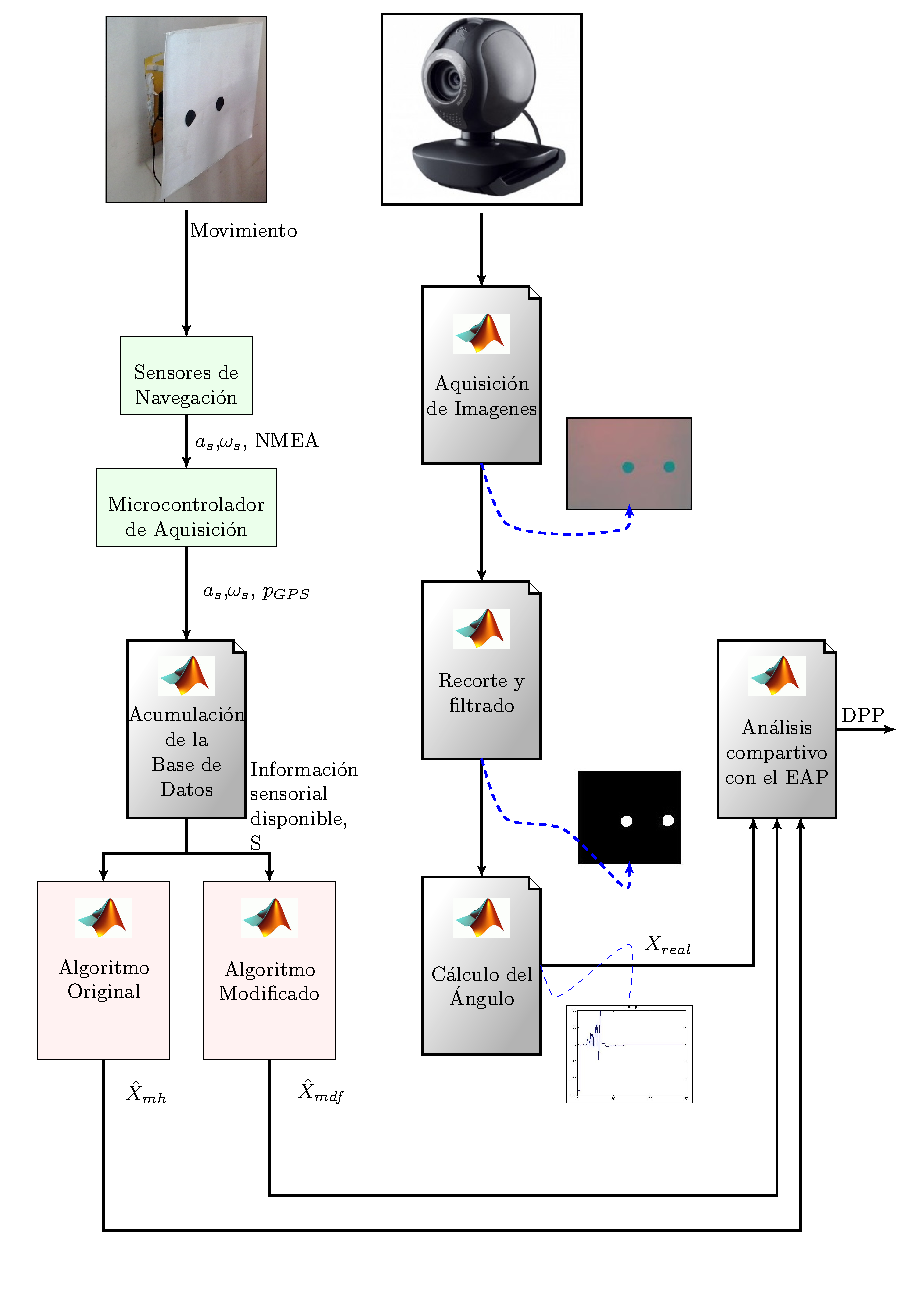
\includegraphics[width=\textwidth]{plataforma_fig10.pdf}
\caption{Esquema general de la plataforma experimental evaluativa.}
\scriptsize{Fuente: Elaboración Propia}
\label{plataforma_fig10}
\end{figure}
La plataforma experimental de la estimación de los ángulos de Euler fue implementada siguiendo el esquema de la Figura \ref{plataforma_fig10}, donde un arreglo de marcas negras en una plancha blanca sujeta a la caja de sensores permite hacer el seguimiento de la evolución del movimiento angular de manera simultánea a la captura de las señales de los sensores de navegación. De esa manera el procesamiento está dividido en dos etapas: primero se sigue el procedimiento descrito en la Figura \ref{plataforma_fig1}, por el cual se obtiene la estimación de la información de navegación $\hat{X}_{mdf}$ y $\hat{X}_{mh}$; posteriormente, de forma paralela se obtiene la información de referencia correspondiente a la evolución temporal de la componente\footnote{De posición angular} sobre la cual se está haciendo el análisis, esta información procede del estudio del desplazamiento de las dos marcas negras capturado en una secuencia de imágenes. La cual es sometida a varios procesos de filtrado para determinar la posición de las marcas y así calcular la progresión de la inclinación equivalente al desplazamiento angular de la variable en estudio, a continuación este procedimiento es descrito en la siguiente secuencia de pasos:
\begin{enumerate}
\item En cada una de las imágenes, para un color en particular\footnote{Se selecciona empíricamente entre las tres matrices de intensidad (rojo, verde y azul) buscando el mejor desempeño en la determinación de las marcas.},  se recorta la zona por donde se mueven las marcas. 
\item Posteriormente, se invierten los colores con la finalidad de resaltar la ausencia de luz\footnote{Debido a su color Negro de las marcas} para después convertirlas en imágenes binarias usando la función \texttt{im2bw(imagen,umbral)} de la \textsl{Image Adquisition Toolbox} de \textsl{MATLAB}, donde el umbral es determinado por prueba-error para cada experimento y condición de iluminación.
\item Con la finalidad de eliminar el ruido introducido por las sombras, en cada una de las imágenes binarias aplicamos el filtro morfológico \texttt{imopen()}, el cual elimina todos los cúmulos aproximadamente circulares con un radio menor a 5 ó 2 pixeles (dependiendo del experimento).
\item Entonces para eliminar totalmente el efecto de las sombras se aplica la función \texttt{imclearborder()}, la cual elimina todas las estructuras morfológicas conectadas al borde.
\item En este punto ya se tiene una secuencia de imagenes depuradas donde solo aparecen las marcas, y corresponde calcular los centriodes de las marcas e identificar cual corresponde a una marca central y cual a una marca externa. Para esto, basados en la función \texttt{colorit()} del apéndice B, se asigna un color a  cada cúmulo\footnote{Que representa a una marca}, despues calculando el centroide se hace la asignación de centro o marca externa basados en cual centroide es más próximo al centro. Este proceso de asignación es seguido en todas las imágenes de la secuencia obteniendo al final dos vectores columna que contienen las coordenadas de las marcas durante todo el desplazamiento.
\item Con los vectores columna de la evolución de la posición vs tiempo tanto del centro como de la marca exterior se determina el ángulo de inclinación, que coincide con la inclinación de los sensores de navegación, ya que la cámara y los sensores están alineados en planos paralelos usando burbujas de albañilería de manera muy cuidadosa.
\end{enumerate}
Esta es una variación del ejemplo \textsl{Length of a Pendulum in Motion} desarrollado por MATLAB. El código implementado en este trabajo se muestra en el apéndice \ref{apen2}.\par
%%
Ahora bien, debido a las características de la plataforma los experimentos desarrollados atacan el análisis de uno de los componentes de los ángulos de Euler a la vez, por lo tanto en cada uno de los ensayos se buscó el cumplimiento de las siguientes condiciones que garantizan que el ángulo determinado en la recta que pasa por los centroides coincida con el ángulo de giro en el parámetro de Euler en cuestión:
\begin{enumerate}
\item El eje de la cámara debe coincidir con el eje de rotación de la caja de los sensores.
\item Dos de los ejes del marco referencial $\marco{A}$ deben formar un plano paralelo al plano de rotación, para así garantizar que el movimiento en los ángulos restantes sea nulo.
\item Y por último, que los ángulos de inclinación de las marcas y la de la caja de sensores estén alineados en cero grados antes de comenzar el movimiento, y así minimizar el \bias en la medición del ángulo con la cámara.
\end{enumerate}
Bajo estas condiciones se hacen tres arreglos distintos para los tres ejes del $\marco{B}$, es decir en $x$ para $\phi$, en $y$ para $\theta$, y en $z$ para $\psi$.
\subsection{Plataforma experimental de la estimación de la posición y velocidad lineal}
Para la evaluación de la estimación de la posición y velocidad lineal el esquema implementado utiliza como sensor adicional un GPS Etrex-Garmin que tiene una precisión de hasta 2 metros, por mucho mayor a la del módulo GPS usado dentro del conjunto de sensores de navegación, esto gracias a la ganancia de su antena que le permite capturar un mayor número de satélites, además de tener una memoria especializada para la captura de datos de Efemérides y Calendarios pasados. Este dispositivo cuenta con un altímetro y una brújula electrónica, mejorando su precisión aún más.\par%%
\begin{figure}[t]
\centering
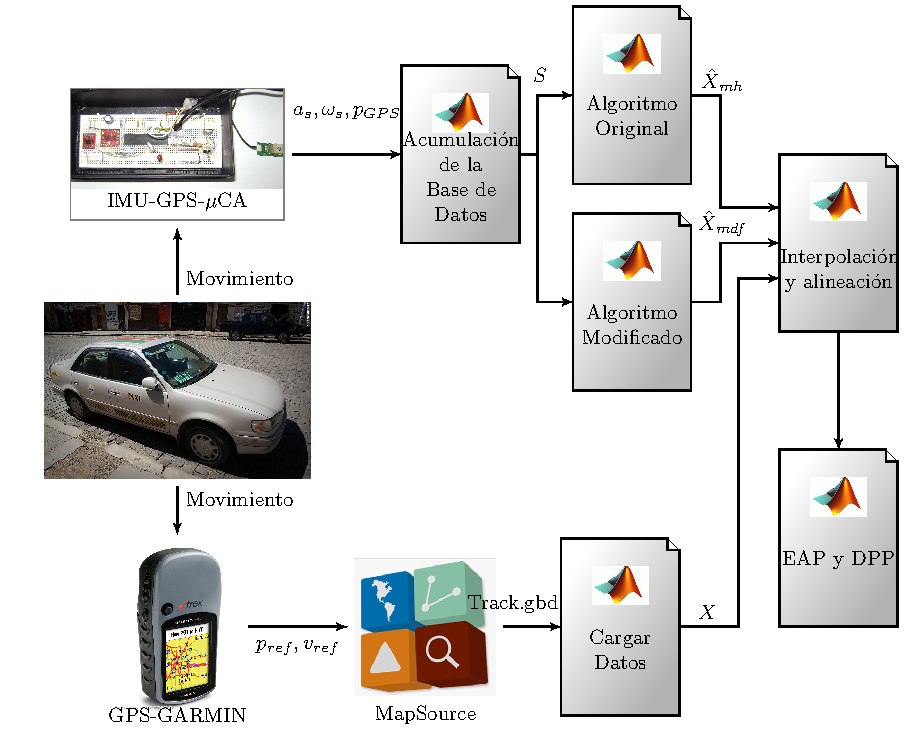
\includegraphics[width=\textwidth]{plataforma_fig11.pdf}
\caption{Esquema de la implementación de la plataforma experimental de la estimación del movimiento lineal.}
\scriptsize{Fuente: Elaboración Propia}
\label{plataforma_fig9}
\end{figure}
Los experimentos son realizados siguiendo circuitos cerrados en un vehículo en donde se monta una caja que contiene al sensor adicional y los sensores de navegación de forma tal que es posible realizar la estimación de la información de navegación y capturar información de referencia. El procedimiento seguido para la captura de esta información es mostrado en el esquema de la Figura \ref{plataforma_fig9}, donde el movimiento del vehículo es capturado simultáneamente por el GPS GARMIN-ETEX y los sensores de navegación, incorporando esta información por medio del programa \texttt{adquiereINS.m}, el cual contiene los comandos de comunicación con el microcontrolador de adquisición; posteriormente esta información, debidamente guardada en $S$, es procesada por los algoritmos de navegación sintetizados en los programas \texttt{ProcesamientoMahonyScan.m} y \texttt{ProcesamientoModificado.m}; en lo que corresponde a GPS GARMIN-ETEX, la información de la orientación de la brújula, la magnitud de la velocidad de desplazamiento y la posición en coordenadas geódicas \footnote{Las que son guardadas en la memoria del dispositivo} es guardada en el archivo \texttt{Track.gdb}, luego extraída y reordenada en el archivo \texttt{Track.xls} utilizando el programa \emph{MapSource}, para que finalmente el programa \texttt{CargarDatos.m} extraiga el historial del movimiento lineal en el marco referencial $\marco{A}$; concluyendo con el proceso, los programas \texttt{Sync.m} sincronizan temporalmente la información estimada y la de referencia siguiendo el periodo de muestro $h$, para posteriormente incorporar las fórmulas de cálculo de los EAP y el DPP.
\subsection{Calibración de los sensores de navegación: Unidad de medida inercial.}
Con la finalidad de obtener mediciones coherentes y asegurar una buena calidad en los datos obtenidos durante el proceso experimental, los sensores deben ser propiamente calibrados. A continuación se detalla el procedimiento seguido para los distintos sensores usados en el presente trabajo.\par
Como ya se menciona, la Unidad de Medida Inercial (IMU, Inertial Measurement Unit) está constituida por un acelerómetro y un giroscopio de tres ejes, los cuales entregan señales eléctricas proporcionales a estos parámetros y que dependen de dos constantes fundamentales: el \bias de medición y el \emph{factor de sensibilidad}. En ese sentido se planifican diferentes ensayos para calcular, específicamente:
\begin{enumerate}
\item Los \bias del acelerómetro.
\item La sensibilidad del acelerómetro.
\item La \bias del giroscopio.
\item La sensibilidad del giroscopio.
\end{enumerate}
A continuación se detallan estos procedimientos.
\subsubsection{Investigación de las direcciones de la medición de la aceleración y la velocidad angular.}
\begin{figure}[t]
\begin{center}
\includegraphics{IMUGPS2.jpg}
\caption{Ejes Coordenados de $\marco{B}$ en la plataforma experimental evaluativa del algoritmo de navegación modificado.}
\label{IMUGPS_fig6}
\end{center}
\scriptsize{En esta figura se muestran los sensores usados, y el microcontrolador de adquisición, los cuales se encuentran fijos al compartimiento. Además, se muestran los ejes alineados con los versores del marco referencial fijo al cuerpo. Fuente: Elaboración Propia}
\end{figure}
Es importante, como se ha planteado en el capítulo dos, que las mediciones de la velocidad angular y la medición de la aceleración se hagan respecto al marco $\marco{A}$.\par
%%
Según el circuito armado, en una \emph{ProtoBoard}\footnote{Tableta de prototipos electrónicos.} buscamos que los ejes estén dispuestos como se muestra en la Figura \ref{IMUGPS_fig6}, de tal forma que movimientos en los ejes entreguen valores positivos de la aceleración. De esa manera, se hizo un experimento relativamente sencillo, el cual consiste en realizar tres movimientos en los tres ejes del marco $\marco{B}$: el primero es un movimiento acelerativo en dirección positiva del eje\footnote{Se habla genéricamente, puede ser cualquiera de los ejes en la direcciones de los versores del marco $\marco{A}$}; el segundo es un movimiento acelerativo hacia la parte negativa del eje; y por último una exposición a la gravedad en sentido positivo del eje, y durante este movimiento se capturan los datos de tal forma que los datos obtenidos son usados para establecer los signos de la aceleración. Durante este experimento también se exploran la positividad de los ejes del giroscopio realizando movimientos dextrogira alrededor de los ejes positivos en el siguiente orden: primero alabeo (en x), luego rodadura (en y) y por último guiñada (en z).\par
%%
Los resultados mostrados en la Figura \ref{obtencion_fig9}, señalan que la aceleración tiene el siguiente comportamiento:
\begin{itemize}
\item \emph{Aceleración en el eje X}: en la gráfica superior se ve el comportamiento de la medición de la aceleración en eje X, donde para el movimiento en sentido positivo se tienen valores negativos y para movimientos hacia el eje negativo se tienen valores positivos, tal como lo señalan los picos negativo y positivo, respectivamente. Esto señala que la aceleración esta invertida en este eje. Ahora para la exposición a la gravedad vemos que existe un incremento de voltaje en este eje, pero como la sensibilidad tiene signo negativo, esto significa que la gravedad está apuntando hacia el eje negativo, aun cuando el eje X positivo apunta hacia abajo.
\item \emph{Aceleración en el eje Y}: en la segunda gráfica se ve el comportamiento de la medición de la aceleración en el eje Y, donde el signo del movimiento coincide con los signos de los ejes, prueba de ello son el primer pico negativo correspondiente a una aceleración, y el segundo pico negativo correspondiente a una aceleración en eje negativo Y. Se debe mencionar que el primer pico indica el sentido del movimiento, y el segundo se debe al efecto de desaceleración. Observamos un efecto decremental cuando la gravedad apunta hacia el eje positivo $Y$, lo que parece indicar que la gravedad tiene un sentido opuesto al natural, el cual apunta hacia el centro de la Tierra.
\item \emph{Aceleración en el eje Z}: aquí vemos un efecto similar al de la aceleración en el eje X, y no indica que la sensibilidad tiene signo negativo respecto a los ejes del marco referencial $\marco{B}$. Aunque no se muestra, el efecto de la gravedad corrobora la suposición de que $g_0$ medida con este acelerómetro tiene signo opuesto al $g_0$ natural.
\end{itemize}
\begin{figure}
\begin{center}
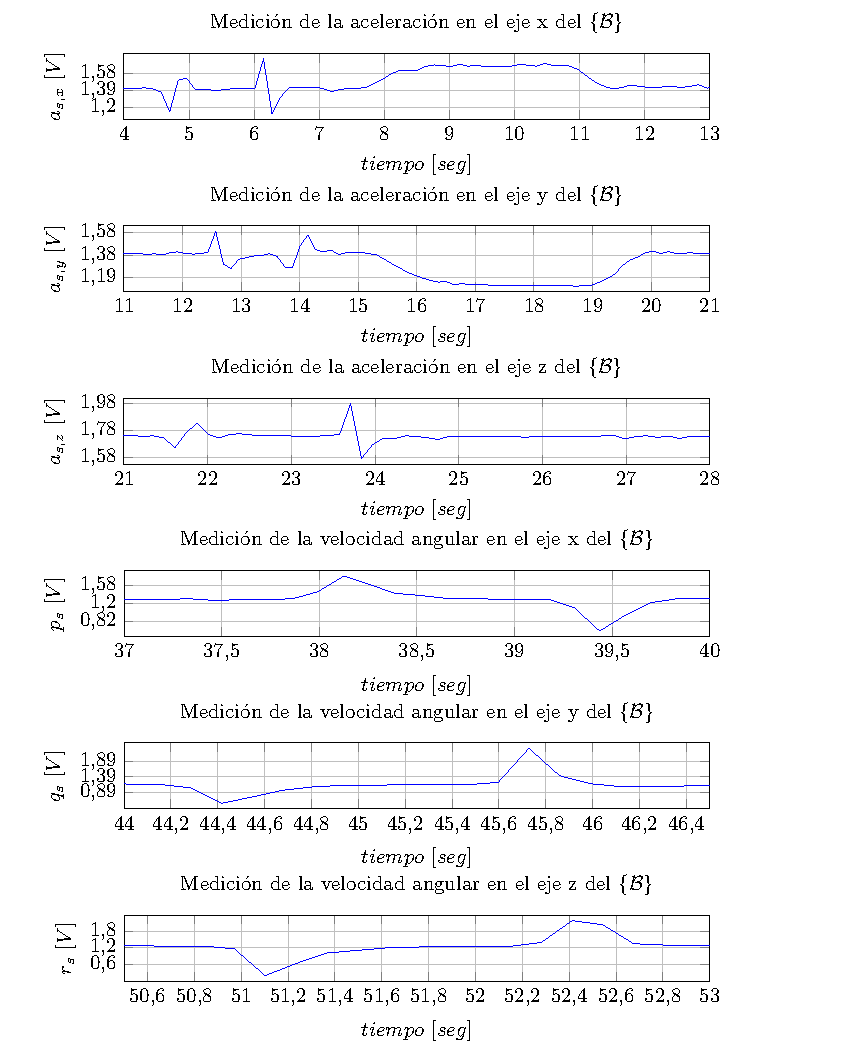
\includegraphics[width=\textwidth]
{PlotIMU2.pdf}
\caption{Señales de la IMU durante el experimento de averiguación de las direcciones de medición de la IMU.}
\scriptsize{El orden corresponde a la aparición, respecto a $a_s$ y $\Omega_s$ Fuente: Elaboración Propia.}
\label{obtencion_fig9}
\end{center}
\end{figure}
Ahora, con respecto a las gráficas de la velocidad angular es evidente que los signos negativos en las sensibilidades de medición corresponden a las velocidades $q$ y $r$, y el signo positivo corresponde a $p$; esto es evidenciable en los picos invertidos para las dos últimas señales mostradas en la Figura \ref{obtencion_fig9}.
\subsubsection{Experimento de determinación del \bias y sensibilidad de la aceleración.}
Este experimento permite conocer los valores del \bias y de la sensibilidad del acelerómetro midiendo las salidas del acelerómetro en tres posiciones, en las los ejes del marco $\marco{B}$ se exponen a la gravedad natural de la Tierra en los dos sentidos (positivo y negativo); con excepción del eje $Z$, debido a la dificultad de acceso a los pines cuando el \emph{ProtoBoard} se encuentra invertido. \par
El procedimiento de la medición de un voltaje para un eje en particular, se realizó buscando el valor extremo\footnote{Ya sea un máximo o un mínimo.}, con la ayuda de un voltímetro, en el eje expuesto a la gravedad; y una vez hallado tal valor se mide los voltajes en los otros ejes usando otro voltímetro.\par

Los resultados de este experimento se muestran en la Tabla \ref{ooekf_tb3}, para un voltaje de alimentación de 2.90[V] fijado con un circuito regulador de tensión, donde es posible encontrar cierta repetitividad en los valores de los ejes no expuestos a la gravedad que permiten caracterizar el \bias del acelerómetro. Y a partir de ello se puede establecer los valores de \bias de aceleración en el promedio de dichos valores, como:
\begin{gather*}
b_{a,x}=1.375[V]\\
b_{a,y}=1.378[V]\\
b_{a,z}=1.455[V]
\end{gather*}
\begin{table}[t]
\begin{center}
\begin{scriptsize}
\begin{tabular}{p{2.5cm}|p{2.5cm}|p{2.5cm}|p{2.5cm}c} \hline
\center\textbf{Característica de la medición}& \center\textbf{Salida del acelerómetro en $x$ [V]}&\center\textbf{Salida del acelerómetro en $y$ [V]}&\center\textbf{Salida del acelerómetro en $z$ [V]}&\\ \hline
%--------------------------------------------------------------------->
Gravedad alineada con $e_3^\mathcal{B}$&1.387&1.374&1.723\\
Gravedad alineada con $e_2^\mathcal{B}$&1.371&1.101&1.464\\
Gravedad contraria a $e_2^\mathcal{B}$&1.371&1.655&1.446\\
Gravedad alineada con $e_1^\mathcal{B}$&1.098&1.377&1.447\\
Gravedad contraria a $e_1^\mathcal{B}$&1.462&1.380&1.450\\ \hline
\end{tabular}
\end{scriptsize}
\caption{Mediciones de los efectos de la alineación de la gravedad en los ejes del marco referencial $\marco{B}$.} 
\label{ooekf_tb3}
\end{center}
\end{table}
Esta tabla también nos permite obtener las sensibilidades para la aceleración de la gravedad de en La Paz, de $9.78m/s^2$, estableciendo, los factores:
\begin{gather*}
S_{a,x}=-3.56[\frac{m/s^2}{V}]\\
S_{a,y}=3.51[\frac{m/s^2}{V}]\\
S_{a,z}=-3.49[\frac{m/s^2}{V}]
\end{gather*}
\subsubsection{Determinación del \bias y el factor de sensibilidad del giroscopio}
Este experimento está dividido en dos partes: en la primera medimos los valores constantes en las salidas del giroscopio para determinar el \bias, lo que deriva en un primer cálculo de esta variable; en una segunda etapa capturamos un conjunto de datos, en donde el circuito de adquisición gira 90º en un sentido\footnote{Ángulo de Euler}, y retorna pasados alrededor de 5 segundo a su posición original, esta información es integrada en un esquema en \textsl{SIMULINK}, que extrae este conjunto de datos del \texttt{workspace} de \textsl{MATLAB} (ver Figura \ref{integrador})
\begin{figure}[t]
\center
\includegraphics[width=\textwidth,viewport=250 250 600 350,clip]{integrador.pdf}
\caption{Esquema de integración en \textsl{SIMULINK}.}
\label{integrador}
\end{figure}
Entonces por ensayo y error se determina el valor de sensibilidad que emula una las salidas con esas características. Un ejemplo de esta gráfica se muestra en la Figura \ref{obtencion_fig10}, en donde la señal es integrada de la velocidad angular en el eje $Z$. Esta señal es el resultado del ajuste del \bias y la sensibilidad del giroscopio del eje Z. \par
De esta manera los valores finales de la sensibilidad y el \bias son:
\begin{figure}[t]
\center
\includegraphics[width=\textwidth]{integrador2.pdf}
\caption{Señal integrada de la velocidad angular $r$.}
\scriptsize{Fuente: Elaboración Propia.}
\label{obtencion_fig10}
\end{figure}
\begin{gather*}
S_{\Omega,p}=-2.3[\frac{mV}{º/s}]\\
S_{\Omega,q}=2.3[\frac{mV}{º/s}]\\
S_{\Omega,r}=-3.1[\frac{mV}{º/s}]
\end{gather*}
Considerando la inversión de los signos en la medición debido al desalineamiento de las direcciones de medición de los giroscopios. El \bias del giroscopio es:
\begin{gather*}
b_{\Omega,p}=1.282[V]\\
b_{\Omega,q}=1.129[V]\\
b_{\Omega,r}=1.2382[V]
\end{gather*}
\subsection{Calibración del sensor angular de video.}
Al momento de hacer la implementación de la plataforma experimental de la estimación de los ángulos de Euler con el sensor de medición angular con la cámara, como ya se menciona, una serie de condiciones deben ser cumplidas para que la medición del ángulo sí corresponda a la que es propiamente realizada por la caja de sensores. Estas condiciones pueden ser resumidas en la Figura \ref{CamAlign}, en la que: el plano de rotación coincide con el plano formado por los ejes del marco $\marco{B}$; y el eje de rotación pasa por el centro de la marca Central y coincide con el eje de la cámara. Lo último es posible tomando como referencia dos superficies perpendiculares, como por ejemplo la pared y el suelo, cuya perpendicularidad es probada usando una escuadra y burbujas de albañilería. \par
%%
\begin{figure}[t]
\center
\includegraphics[width=\textwidth]{CamAlign.pdf}
\caption{Vista lateral de las condiciones de alineación de la cámara, la plancha de marcas y la IMU, referente a una pared vertical.}
\label{CamAlign}
\end{figure}
El procedimiento inicial del armado de la plataforma requiere cierto cuidado, de forma tal que se reduzcan al máximo los errores de alineación en los ejes. Para ello, se sigue el siguiente procedimiento: primero fijamos la plancha blanca buscando que esta quede paralela con una de las caras de la caja de sensores, y así sea paralela al plano de rotación definido por uno de los tres versores del marco $\marco{B}$; después fijamos la marcas a la plancha blanca, de forma tal que la marca central esté centrada en el eje de rotación, definido por eje del rodamiento al que va sujeta la caja de sensores; seguido, con la ayuda de una escuadra y dos burbujas de albañilería perpendiculares entre sí, se alinea eje de rotación (paralelo a alguno de los versores de $\marco{B}$) perpendicular a la superficie de apoyo o sujeción; por último, montado en un pedestal se posiciona la cámara posicionando la marca central al centro del cuadro.\par
%% 
Ahora bien, a pesar de que el armado del arreglo experimental se ha realizado con mucho cuidado es posible que exista pequeñas desviaciones no controladas que se propaguen a la medición del ángulo, entre estos problemas podemos mencionar: 
\begin{itemize}
\item Desviaciones de la marca central proporcionales a la posición angular, las cuales pueden ser atribuidas a una desalineación del eje de la cámara con el eje de rotación o desviaciones de la marca central con respecto al eje de rotación
\item Como un segundo caso, es probable que se tenga un error constante en la medición del ángulo causado por la desviación vertical de la marca externa respecto  a uno de los ejes del marco $\marco{B}$.
\end{itemize}
Considerando esto, en cada prueba se debe realizar un reajuste, ya sea de las marcas ó la inclinación de la caja de sensores. A continuación se describe cada uno de ellos:
\begin{itemize}
\item Marca Externa: poniendo la caja de sensores en posición horizontal, es decir poniendo el ángulo a cero, se calcula la inclinación constante introducida por un mal posicionamiento de la marca externa. Se mueve la marca externa buscando reducir esta inclinación a cero.
\item Inclinación de la caja de sensores: se incrementan o rebajan los topes que soportan a la caja de sensores, buscando la horizontalidad en diferentes posiciones angulares.
\item Marca central: si la marca central está desalineada se hace girar la caja de sensores 360º, lo que permite encontrar visualmente el punto de intersección del eje de rotación y el plano de la plancha. La marca central será movida a este punto.
\end{itemize}
%%%%%%%%%%%%%%%%%%%%%%%%%
%%%%%%%%%%%%%%%%%%%%%%%%%
%%% Seccion VI %%%
%%%%%%%%%%%%%%%%%%%%%%%%%
%%%%%%%%%%%%%%%%%%%%%%%%%
\section{Pruebas experimentales}
Una vez detalladas las plataformas experimentales corresponde hacer la descripción del proceso experimental seguido para indagar en la veracidad de la suposición ya descrita en la Sección \ref{Propuesta} -la cual se constituye en el principal aporte del presente trabajo- la cual afirma que:
\begin{quote}
La inclusión de un Observador Óptimo EKF para la reconstrucción de la matriz de rotación en el esquema de observadores tipo filtro complementario en $SO(3)$ mejora la estimación de la información de navegación.
\end{quote}
La estrategia abordada para cumplir con tal objetivo divide el total de la prueba en dos partes:
\begin{itemize}
\item La prueba para el estudio del desempeño de la estimación de los ángulos de Euler.
\item La prueba para el estudio del desempeño de la estimación de movimiento lineal, es decir la posición y la velocidad lineal.
\end{itemize}
De esa manera, y siguiendo esta secuencia, en esta sección se detalla el procedimiento experimental seguido en la realización de estas dos pruebas.
\subsection{Prueba con la plataforma experimental de la estimación los ángulos de Euler}
Esta fase emplea el esquema experimental descrito en la sección \ref{Plataforma2}, en la cual el sensor angular de video (constituido por una cámara) captura la información de la rotación de uno de los ángulos de Euler, al mismo tiempo que los algoritmos de navegación realizan la estimación de la misma variable\footnote{Dentro del conjunto de datos que conforman la información de navegación estimada.}.\par
%%%
Es importante señalar que debido a que el esquema del sensor angular de video solo puede medir un ángulo al mismo tiempo, el estudio se concreta sobre tres arreglos distintos, en los cuales se varía la disposición de los elementos que constituyen esta plataforma experimental\footnote{Plataforma experimental de la estimación de los ángulos de Euler (ver Figura \ref{plataforma_fig10})}:
\begin{enumerate}
\item \emph{El arreglo para el estudio del ángulo de alabeo $\phi$}. En este los elementos están configurados de tal forma que: el eje de rotación es paralelo al eje $x$ del marco $\marco{B}$; la plancha de las marcas (que se constituye como el plano de rotación) es paralelo al plano $YZ$, con las componentes $z$ apuntando hacia el centro de la tierra y $y$ hacia la izquierda de la imagen\footnote{Cuando la caja de sensores se encuentra con la cara inferior mirando hacia el suelo}. Con lo que respecta a la cámara esta se encuentra en posición vertical tal como se muestra en la Figura \ref{CamAlign}, a una distancia suficiente para enfocar toda la escena de la rotación.
\item \emph{El arreglo para el estudio del ángulo de rodadura $\theta$}. Aquí el eje de rotación es paralelo al eje $y$ del marco $\marco{B}$, el plano de rotación queda en el plano $XZ$, con la componente $z$ (una vez más) apuntando hacia abajo y $x$ apuntando hacia la derecha de la imagen.
\item \emph{El arreglo para el estudio del ángulo de guiñeo $\psi$}. Aquí la configuración cambia radicalmente. En este caso el eje de rotación es paralelo a eje $z$ y perpendicular al plano de rotación sobre el plano $XY$; el versor de $z$ está apuntando hacia abajo en sentido contrario a la posición de la cámara, la cual en este caso está ubicada encima de la caja de sensores; con respecto a los ejes $x$ y $y$, estos apuntan hacia arriba y la izquierda de la imagen tomada por la cámara.
\end{enumerate}
En resumen, en cada uno de los arreglos se realizan varios ensayos, los cuales consisten en la captura de la información de la rotación: en una dimensión para el sensor angular de video, y tres dimensiones para los algoritmos de navegación; de forma tal que tras cada ensayo, si las condiciones de alineación y calibración fueron satisfactoriamente cumplidas, se obtiene como resultado tres señales: la estimación del algoritmo modificado, la estimación del algoritmo original y la medición del sensor angular de video como señal de referencia.\par
El procedimiento seguido en cada uno de los ensayos sigue la siguiente secuencia: primero, se enciende el sensor angular de video; después se mueve la marca externa cerca a los cero grados; se inicia la captura del movimiento junto con el arranque del programa \texttt{AdquiereINS.m}; al terminar la adquisición de los datos, estos se guardan en un archivo \texttt{.mat}; y empleado este archivo, finalmente se procede a calcular las estimaciones de la información de navegación con los programas \texttt{AlgoritmoModificado.m} y \texttt{AlgoritmoOriginal.m}. Aunque entre ensayos varían, en general el movimiento comienza con los ángulos inicialmente alineados\footnote{Esto considerando los dos elementos, es decir la caja de sensores y la plataforma de marcas.} cerca de $0º$, después varían con diferentes velocidades angulares y sentidos de giro durante un periodo de tiempo, el movimiento termina otra vez cerca a los $0º$. En todos los ensayos, se buscó con prioridad mantener los planos de rotación lo más paralelos posible, considerando un ensayo como exitoso solo cuando esta condición se cumple.
%%%
\subsubsection{Resultados de la estimación del ángulo de alabeo.}
Los datos obtenidos de uno de los varios ensayos realizados para esta variable se muestran en la gráfica de la Figura \ref{PlotPh1}, donde la señal de color azul corresponde a la estimación, la de color verde para el  algoritmo original, y de color rojo para la referencia; además, la gráfica superior corresponde a toda la duración del ensayo y la gráfica inferior es el acercamiento del recuadro en color magenta.\par
%%
En este ensayo el movimiento inicia en -2º y termina en poco menos de -3º y los ángulos de rodadura y guiñeo se mantienen en 0º. Para la estimación con el algoritmo modificado los errores oscilan entre $9.04E-4º$ y $10.58º$ en contraste a los $7.33E-3º$ a $18.97º$\footnote{Estos valores están en valor absoluto respecto a la señal original.} para el algoritmo original. 
\begin{figure}
\begin{center}
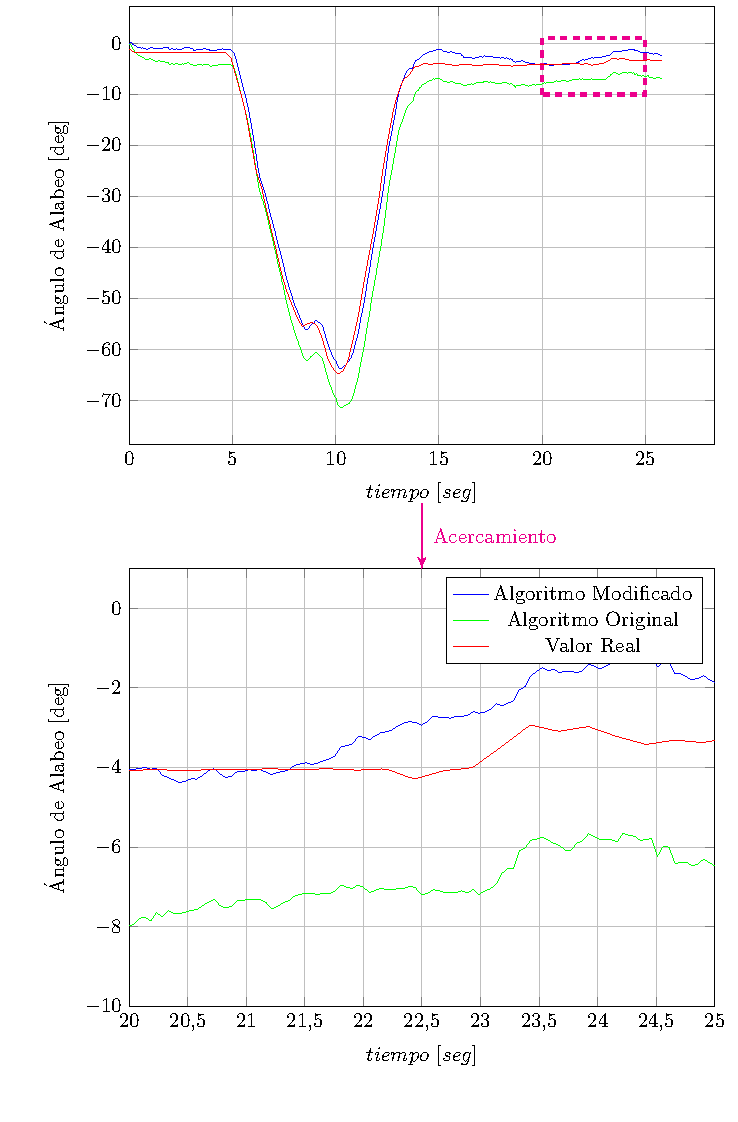
\includegraphics[scale=0.8]
{PlotPh25a.pdf}
\caption{Comparación del desempeño de la estimación del ángulo de alabeo.}
\scriptsize{Resultados de la estimación de con datos simulados. Resultados típicos del repetidos intentos.}
\label{PlotPh1}
\end{center}
\end{figure}
En promedio los errores absolutos (EAP) para estos algoritmos corresponden:
\begin{equation*}
EAP_{mdf,\phi}=1.3579º~\text{Para el algoritmo modificado.}
\end{equation*}
\begin{equation*}
EAP_{mh,\phi}=3.756º~\text{Para el algoritmo original.}
\end{equation*}
%%%
En estas gráficas los errores cometidos por el algoritmo original son mucho mayores a los del algoritmo modificado, donde este último gana definitivamente a partir de 15 segundos. Es también visible que al final hay una tendencia, para ambos algoritmos de acercarse a la señal de referencia.
\subsubsection{Resultados de la estimación del ángulo de rodadura.}
Los resultados de los ensayos muestran una tendencia de superioridad del método modificado respecto al original. Uno de estos ensayos se muestra en la gráfica de la Figura \ref{PlotPh1}, donde una vez más la gráfica de color azul corresponde a la estimación usando el algoritmo modificado, la de color verde para el algoritmo original y la referencial en color rojo. \par
A diferencia del ensayo mostrado anteriormente, en este ensayo los movimientos son mucho más rápidos, los cuales quedan limitados dentro de la banda de $\pm45[º/s]$. Una vez más en este ensayo, el desempeño del algoritmo modificado mejora sobre al algoritmo original, y a partir de los 13 segundos la convergencia del método modificado es insuperable. En la gráfica de acercamiento (que se delimita por la el rectángulo de color magenta) podemos observar el efecto de un golpe en la caja de sensores que inicia a los 21 segundos, que si bien es accidental muestra el tiempo de convergencia de 4 a 5 segundos para el algoritmo modificado.\par
\begin{figure}
\begin{center}
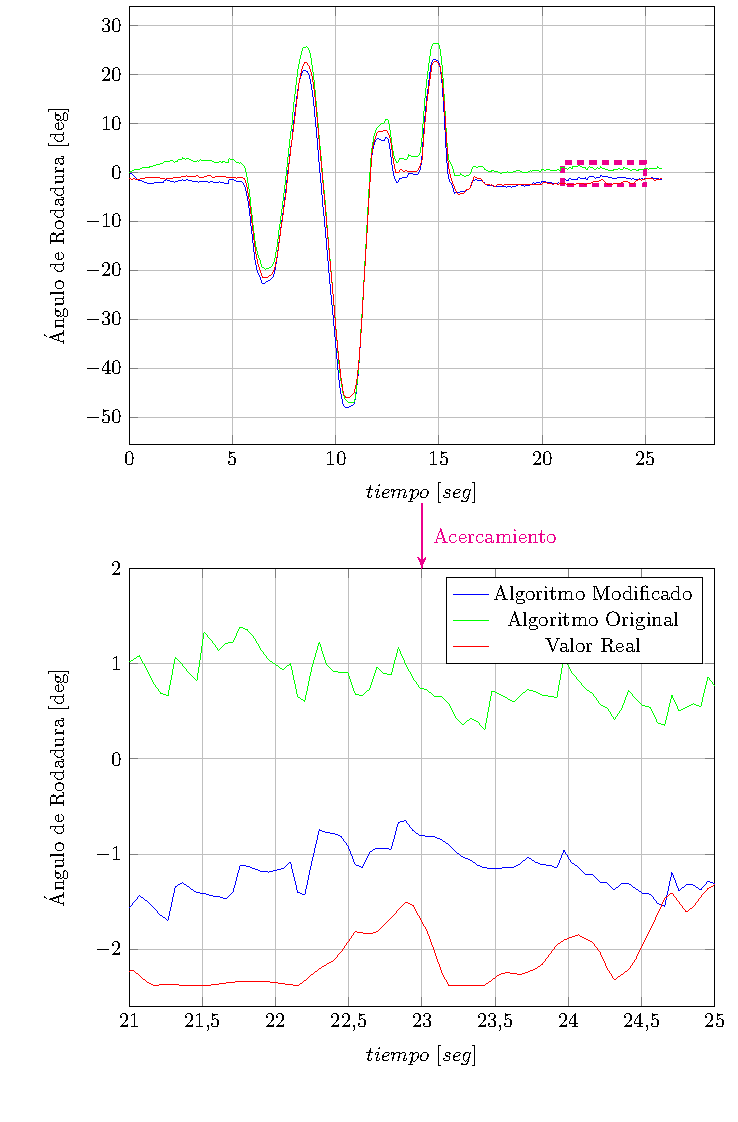
\includegraphics[scale=0.8]
{PlotTh27.pdf}
\caption{Comparación del desempeño de la estimación del ángulo de rodadura.}
\scriptsize{Resultados de la estimación de con datos simulados. Resultados típicos del repetidos intentos.}
\label{PlotTh1}
\end{center}
\end{figure}
Ahora los EAP's para este ensayo son:
\begin{equation*}
EAP_{mdf,\theta}=1.4635º~\text{Para el algoritmo modificado.}
\end{equation*}
\begin{equation*}
EAP_{ms,\theta}=7.072º~\text{Para el algoritmo original.}
\end{equation*}
%%%
Una vez más la gráficas muestran que los errores cometidos por el algoritmo original son mucho mayores a los del algoritmo modificado.\par
La convergencia para el método modificado empieza a ser fiel iniciando los 13 a 14 segundos (ver gráfica), en contraste con el método original en el cual la convergencia no llega en la ventana temporal que dura el experimento; aunque parece que al final hay una cierta tendencia. \par
%%
Ahora, es posible que esto de deba a que a pesar de haber reducido el error constante en la medición durante el proceso de calibración del arreglo, queden residuos que favorezcan al método modificado; si este es el caso, se ve que el golpe no perturba en demasía el valor final encontrado por el algoritmo original, de lo cual podemos decir que tiene cierto grado de robustez superior a la desempeñada por el algoritmo modificado.\par 
%%%
\subsubsection{Resultados de la estimación del ángulo de guiñada}
Para la componente de guiñada los ensayos fueron realizados con la plataforma en posición horizontal dando al sistema mayor movilidad. Con estas características, en este arreglo se pudieron alcanzar velocidades angulares mucho mayores a la de los otros experimentos. Sin embargo, se hace importante mencionar que en estas condiciones el vector gravitacional está apuntando paralelo al eje de rotación, dificultando la estimación vectorial y así la estimación del ángulo de guiñeo para el algoritmo original; por esta razón la capacidad de convergencia del método original, cuando la condición inicial del ángulo muy distinta de cero, se ve afectada considerablemente.\par
%%
En la Figura \ref{PlotPs1} se muestra los resultados de la estimación del ángulo de guiñeo. Específicamente en este experimento el ángulo inicial de guiñeo es de 5º, lo que permite ver el efecto anteriormente mencionado, donde a pesar de que las condiciones iniciales de los ángulos de Euler en los algoritmos de navegación son nulas, el algoritmo modificado reduce progresivamente el error, en contraste con el algoritmo original, el cual permanece con un error constante de 1.5º (como se muestra en el acercamiento), por lo menos durante toda la ventana temporal que dura el experimento.\par
\begin{figure}
\begin{center}
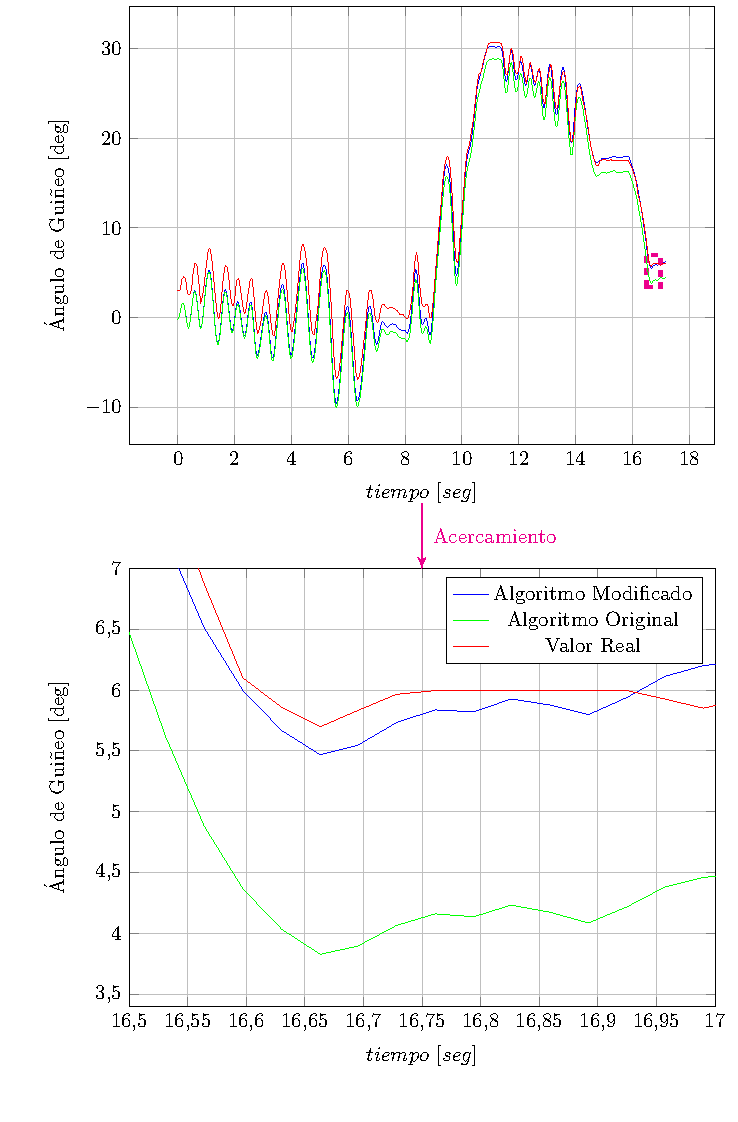
\includegraphics{PlotPs11.pdf}
\caption{Comparación del desempeño de la estimación del ángulo de guiñeo.}
\scriptsize{Resultados de la estimación de con datos simulados. Resultados típicos del repetidos intentos.}
\label{PlotPs1}
\end{center}
\end{figure}
En cuanto al tiempo de convergencia, de forma reiterada en todos los ángulos muestra que la convergencia siempre está cerca de los 12 segundos, y a partir de ese tiempo se sigue fielmente la referencia.\par
En este ensayo los EAP simplemente corroboran la evidente ventaja de método modificado frente al original.
\begin{equation*}
EAP_{mdf,\psi}=1.4635º~\text{Para el algoritmo modificado.}
\end{equation*}
\begin{equation*}
EAP_{ms,\psi}=7.072º~\text{Para el algoritmo original.}
\end{equation*}\newpage
\subsection{Prueba con la plataforma experimental de la estimación del movimiento lineal}
Los experimentos realizados con esta plataforma permiten ver el desempeño del algoritmo para estimar el movimiento lineal, es decir la velocidad lineal y la posición en el tiempo. \par
\begin{figure}[ht]
\begin{center}
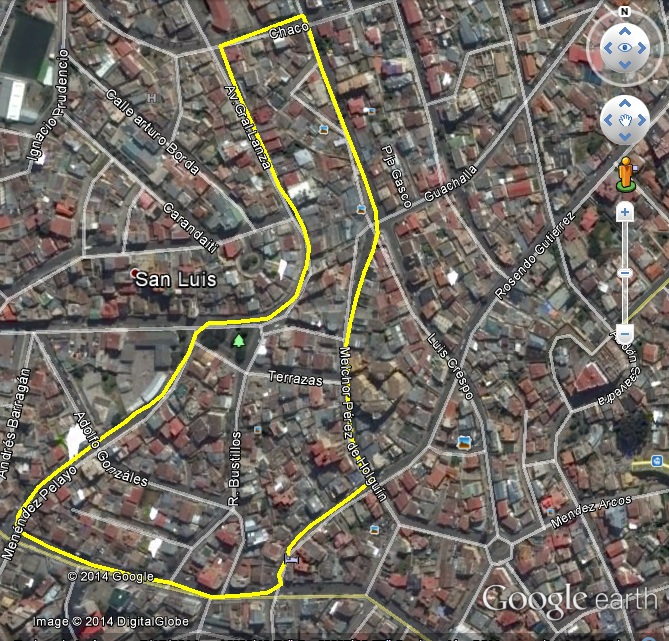
\includegraphics[width=\textwidth]
{pruebas_fig1a.jpg}
\caption{Circuito cerrado de las pruebas con la plataforma experimental de la estimación del movimiento lineal.}
\text{Fuente: Google Earth y DigitalGlobe 2013}
\label{pruebas_fig1}
\end{center}
\end{figure}
Los ensayos se desarrollan en un circuito cerrado delimitado en la zona de Sopocachi Alto\footnote{Zona seleccionada por sus facilidades logísticas.} con los sensores montados en un vehículo. Esta ruta, mostrada en la Figura \ref{pruebas_fig1}, tiene una longitud de $1.53[Km]$, pasa por calles con buena línea de vista, sin muchos árboles\footnote{Podados por la época del año.} ni edificios. En cada ensayo se siguió el siguiente protocolo:	
\begin{enumerate}
\item Se hace la alineación al norte tanto del GPS-GARMIN-ETREX, como la del marco referencial $\marco{B}$, para que las condiciones iniciales en los ángulos de Euler sean nulas.
\item Se inicia el programa de \texttt{AdquiereINS.m}.
\item Se hace el desplazamiento con velocidades de hasta $20[kph]$.
\item Y por último se guarda los datos adquiridos para comenzar con el siguiente ensayo, si corresponde.
\end{enumerate}
A continuación se describen los resultados obtenidos de las pruebas que se pudieron realizar, señalando que no fueron muchas debido a un tema de disponibilidad de equipos.
\subsubsection{Resultados de la estimación de la posición}
Como ya se señala las pruebas fueron realizadas en un radiotaxi siguiendo la ruta de la Figura \ref{pruebas_fig1}. En esta ruta las calles con mayor conflicto de línea de visión del GPS debido a la proximidad de los edificios fueron la c/ Melchor Pérez de Holguín y la c/ Chaco.\par
%%
\begin{figure}
\begin{center}
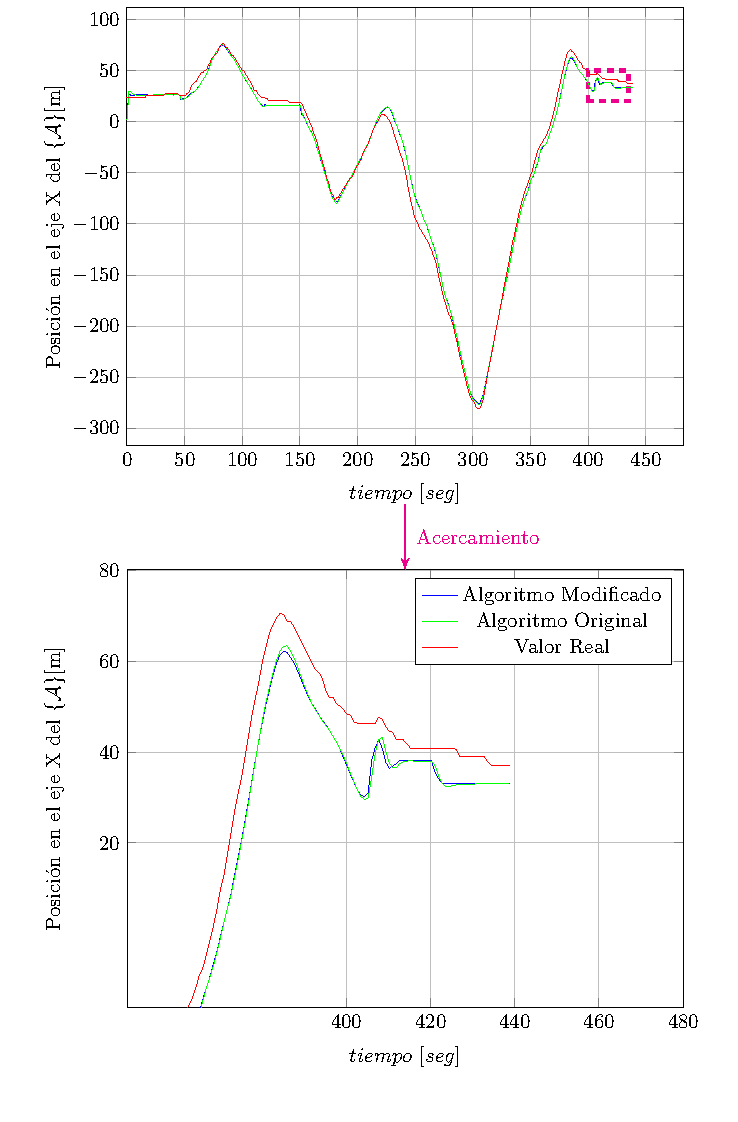
\includegraphics[scale=0.8]
{PlotX4b.pdf}
\caption{Comparación del desempeño de la estimación de la posición en el eje X.}
\scriptsize{Resultados de la estimación de con datos simulados. Resultados típicos del repetidos intentos.}
\label{PlotX1}
\end{center}
\end{figure}
%%
\begin{figure}
\begin{center}
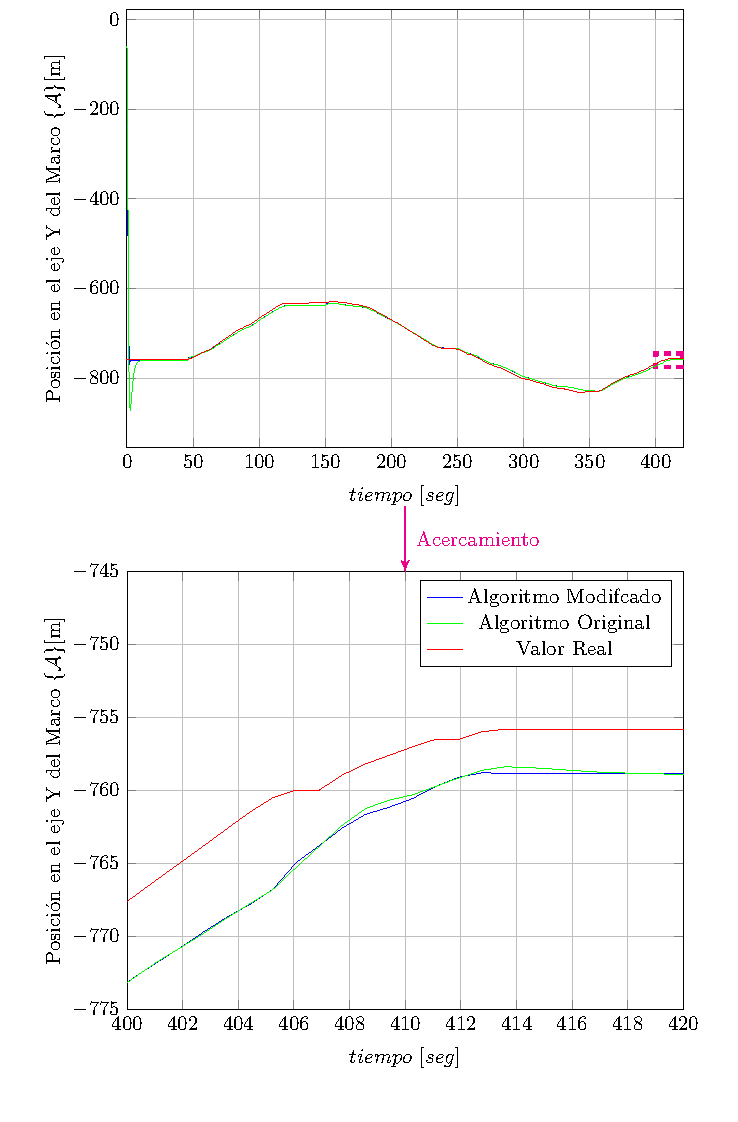
\includegraphics[scale=0.8]
{PlotY4b.pdf}
\caption{Comparación del desempeño de la estimación de la posición en el eje Y.}
\scriptsize{Resultados de la estimación de con datos simulados. Resultados típicos del repetidos intentos.}
\label{PlotY1}
\end{center}
\end{figure}
%%%
\begin{figure}
\begin{center}
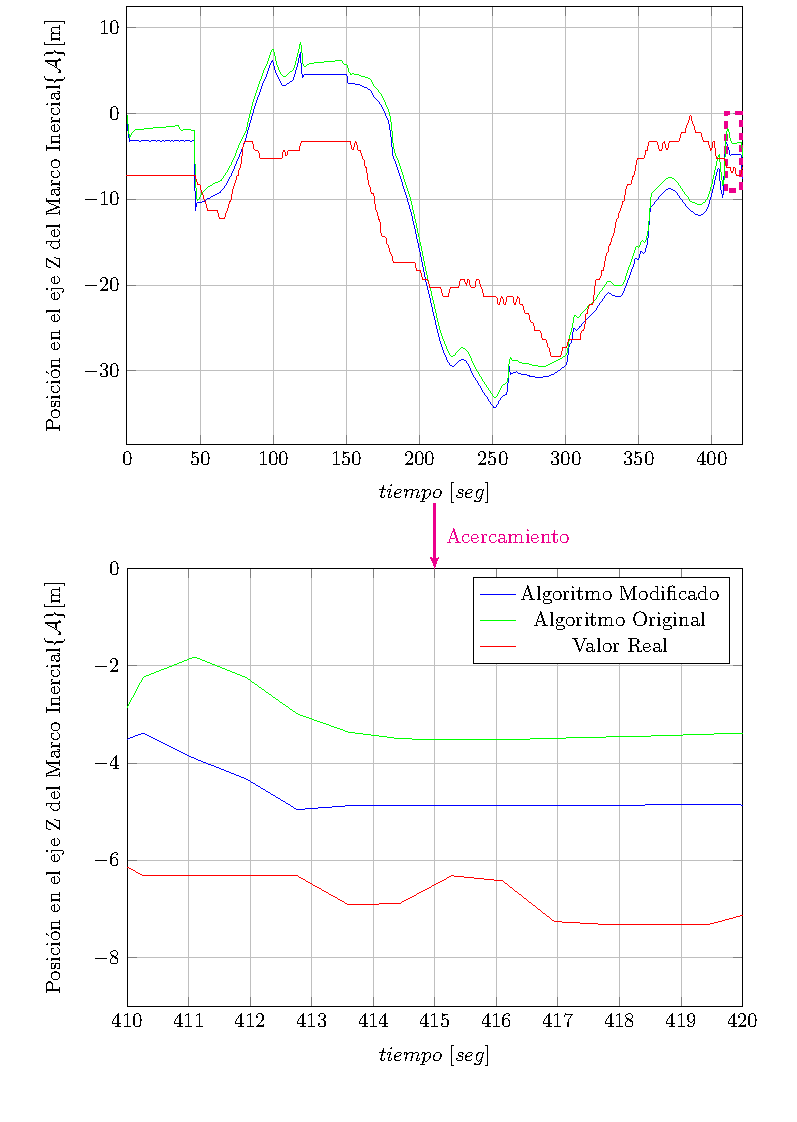
\includegraphics[scale=0.8]
{PlotZ4b.pdf}
\caption{Comparación del desempeño de la estimación de la posición en el eje Z.}
\scriptsize{Resultados de la estimación de con datos simulados. Resultados típicos del repetidos intentos.}
\label{PlotZ1}
\end{center}
\end{figure}
%%%
En todas las gráficas, los resultados de la estimación del algoritmo Original son representados en la línea de color verde, para la estimación del algoritmo modificado de color azul, y para la señal de referencia en una línea de color rojo. Estos resultados son mostrados en las Figuras \ref{PlotX1}, \ref{PlotY1} y \ref{PlotZ1}. Este ensayo dura 421 segundos ó 7 minutos 1 segundo, y durante todo este tiempo se puede observar, que si bien la estimación sigue la señal de referencia esta mantiene un error durante toda la trayectoria, esto para ambos algoritmos. Sin embargo, dado que la diferencia entre las dos estimaciones es muy pequeña, el tema del error no afecta a la suposición que se trata de refutar o afirmar, dado que se habla de cual de los algoritmos estima mejor, y a pesar de que ambos estén equivocados, la competencia está en cual es más próximo al valor verdadero.\par
%%
Por su parte, este error puede ser cuantificado en el EAP para cada una de las gráficas, donde el sub-índice $mdf$ significa que pertenece al algoritmo modificado y $mh$ significa que pertenece al algoritmo original:
\begin{equation*}
EAP_{mdf,x}=5.8290 [m]~\text{Para el algoritmo modificado.}
\end{equation*}
\begin{equation*}
EAP_{ms,x}=5.8976 [m]~\text{Para el algoritmo original.}
\end{equation*}
\begin{equation*}
EAP_{mdf,y}=3.5046 [m]~\text{Para el algoritmo modificado.}
\end{equation*}
\begin{equation*}
EAP_{ms,y}=4.6888 [m]~\text{Para el algoritmo original.}
\end{equation*}
\begin{equation*}
EAP_{mdf,z}=6.1602 [m]~\text{Para el algoritmo modificado.}
\end{equation*}
\begin{equation*}
EAP_{ms,z}=6.2365 [m]~\text{Para el algoritmo original.}
\end{equation*}
Respecto a las gráficas de las Figuras \ref{PlotX1} y \ref{PlotY1}, la gráfica de la Figura \ref{PlotZ1} parece la más imprecisa, sin embargo hay que considerar que los errores en la altitud son uno de los mayores defectos del sistema GPS, y típicamente son grandes\footnote{Esto no pone en cuestión la veracidad de la información entregada por el GPS-Garmin, debido a que este dispositivo utiliza la información de un barómetro, que sin duda tiene mejor precisión.}. A pesar de eso, es de consideración ver que la información estimada se aproxima a la señal de referencia, mucho más que la medición del sensor de navegación GPS-MTK3329. 
\subsubsection{Resultados de la estimación de la velocidad lineal.}
En esta prueba, dado que la velocidad de referencia esta expresada en el marco referencial inercial $\marco{A}$ y la medición de la aceleración, de donde se obtiene la estimación, está expresada en el marco referencial fijo al cuerpo $\marco{B}$, se hace inevitable utilizar la matriz de rotación $R$ (definida en la sección \ref{RotationMatrix}) para hacer la transformación correspondiente. Entonces, esto sugiere que la convergencia está delimitada por la capacidad de los algoritmos para estimar los ángulos de Euler. Los resultados de las pruebas realizadas son mostrados en las Figuras \ref{PlotU1}, \ref{PlotV1} y \ref{PlotW1}, en las que se muestran la velocidad en $x$, $y$ y $z$ del marco referencial inercial $\marco{A}$ con la misma notación de colores que se ha venido manteniendo desde la Figura \ref{PlotPh1}.\par
\begin{figure}
\begin{center}
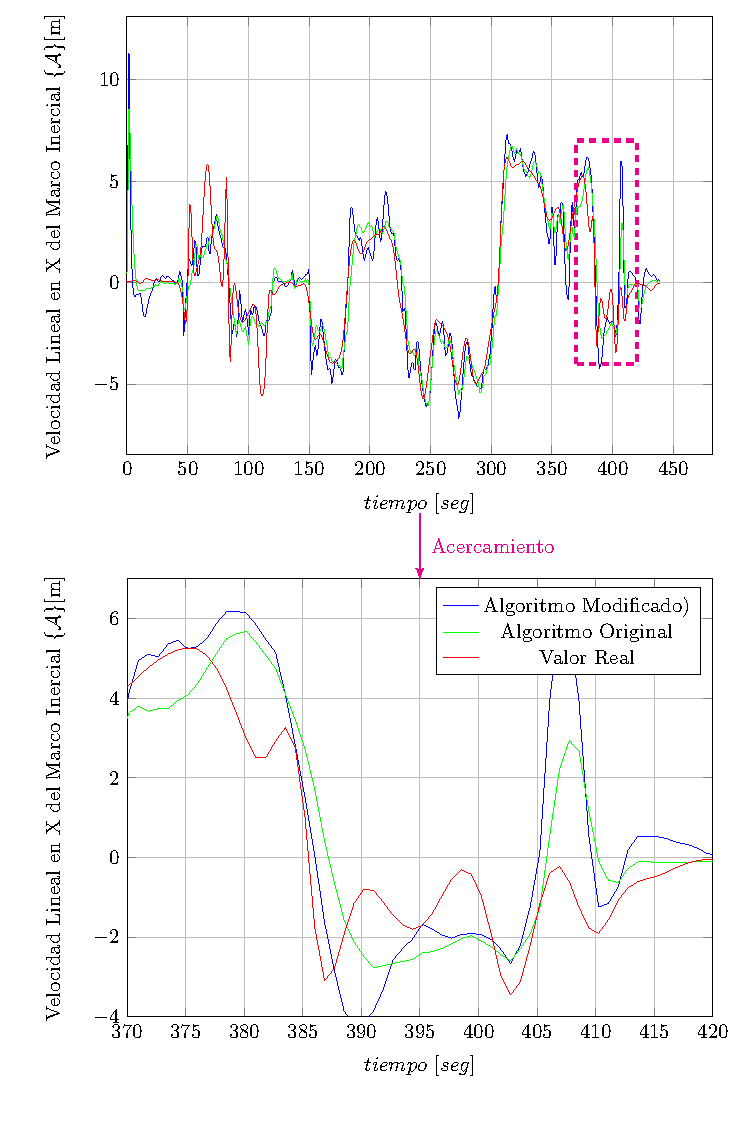
\includegraphics[scale=0.8]
{PlotU.pdf}
\caption{Comparación del desempeño de la estimación de la velocidad lineal en el eje X.}
\scriptsize{Resultados de la estimación de con datos simulados. Resultados típicos del repetidos intentos.}
\label{PlotU1}
\end{center}
\end{figure}
%%%
En estas gráficas, a pesar de que los errores de la estimación de la posición son bastante grandes\footnote{Para ciertas aplicaciones.}, la estimación de la velocidad parece mucho más certera. Y se observa una ventaja evidente del método modificado frente al original, lo que es positivo para la suposición investigada. Este argumento se refuerza con los valores de los errores absolutos promedio para cada una de las tres variables, denotados a continuación:
\begin{equation*}
EAP_{mdf,u}=0.8958 [m/s]~\text{Para el algoritmo modificado.}
\end{equation*}
\begin{equation*}
EAP_{ms,u}=0.7871 [m/s]~\text{Para el algoritmo original.}
\end{equation*}
\begin{equation*}
EAP_{mdf,v}=3.1564 [m/s]~\text{Para el algoritmo modificado.}
\end{equation*}
\begin{equation*}
EAP_{ms,v}=3.3291 [m/s]~\text{Para el algoritmo original.}
\end{equation*}
\begin{equation*}
EAP_{mdf,w}=0.3476 [m/s]~\text{Para el algoritmo modificado.}
\end{equation*}
\begin{equation*}
EAP_{ms,w}=0.64 [m/s]~\text{Para el algoritmo original.}
\end{equation*}
\begin{figure}
\begin{center}
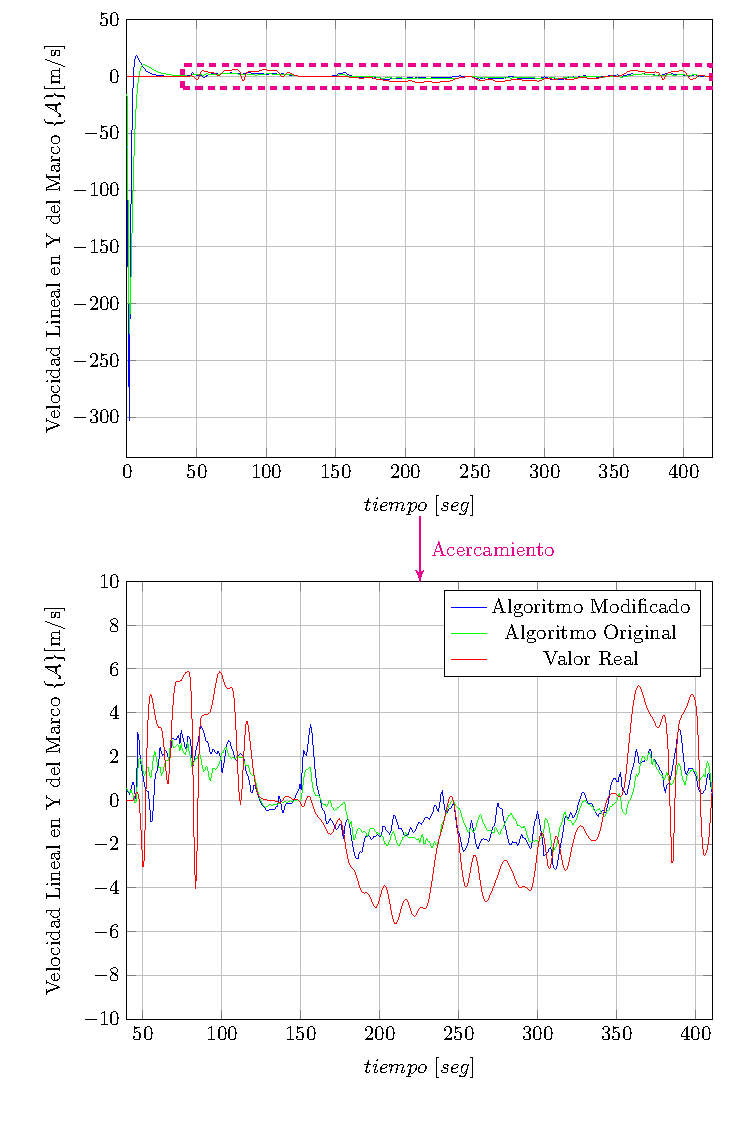
\includegraphics[scale=0.8]
{PlotV.pdf}
\caption{Comparación del desempeño de la estimación de la velocidad lineal en el eje Y.}
\scriptsize{Resultados de la estimación de con datos simulados. Resultados típicos del repetidos intentos.}
\label{PlotV1}
\end{center}
\end{figure}
%%%
\begin{figure}
\begin{center}
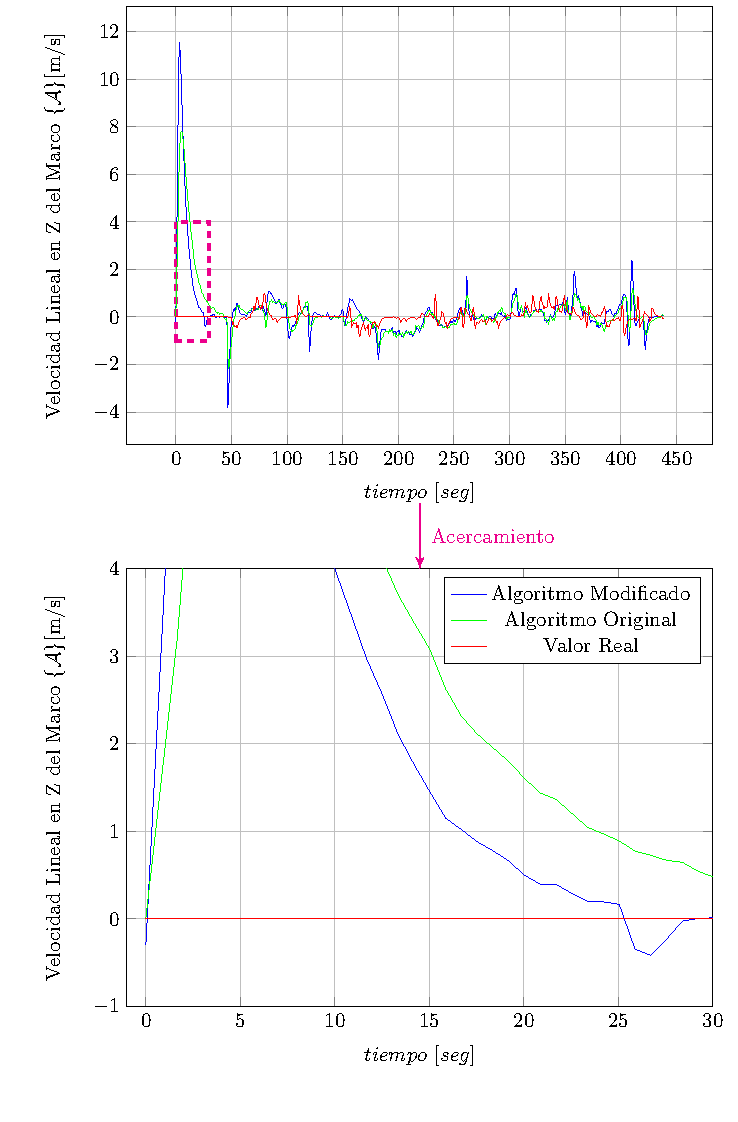
\includegraphics[scale=0.8]
{PlotW.pdf}
\caption{Comparación del desempeño de la estimación de la velocidad lineal en el eje Z.}
\scriptsize{Resultados de la estimación de con datos simulados. Resultados típicos del repetidos intentos.}
\label{PlotW1}
\end{center}
\end{figure}
\newpage
\subsection{Resultados del Análisis Comparativo con el EAP y el DPP.}
Como se menciona en la anterior sección después de obtener las señales estimadas por los algoritmos de navegación se prosigue con el análisis comparativo con el EAP y el DPP. En la Tabla \ref{resultados_tb1} se ordenan los EAP y las diferencias porcentuales para cada variable.\par
\begin{table}
\begin{center}
\begin{tabular}{|p{2in}|p{1.0in}|p{1.0in}|p{1.0in}|} \hline
\textbf{Variable estimada}&\small\textbf{Error Absoluto Promedio del algoritmo modificado}&\small\textbf{Error Absoluto Promedio del algoritmo original}&\small\textbf{Diferencia Porcentual del Algoritmo Modificado respecto al Original.} \\ \hline
%--------------------------------------------------------------------->
Posición en el eje X ($x$) &5.8862[m]&5.9427[m]&0.9596\%\\ \hline
Posición en el eje Y ($y$) &3.5445[m]&4.7739[m]&34.6828\%\\ \hline
Posición en el eje Z ($z$)&6.1698[m]&6.3369[m]&2.7080\%\\ \hline
Velocidad lineal en el eje X ($v_x$) &0.8214[m/s]&0.7871[m/s]&\textcolor{red}{-12.1305\%}\\ \hline
Velocidad lineal en el eje Y ($v_y)$&3.1564[m/s]&3.3291[m/s]&5.4710\%\\ \hline
Velocidad lineal en el eje Z ($v_z$)&0.4445[m/s]&0.5697[m/s]&28.1664\%\\ \hline
Ángulo de alabeo ($\phi$ )&1.3579[Deg]&3.7560[Deg]&177.97\%\\ \hline
Ángulo de rodadura ($\theta$ )&1.4635[Deg]&2.801[Deg]&91.394\%\\ \hline
Ángulo de guiñeo ($\psi$ )&1.3268[Deg]&2.1855[Deg]&44.53\%\\ \hline
\end{tabular}
\caption{Tabla comparativa del desempeño de Algoritmo de tres observadores en cascada y el de Mahony-Scandaroli.}
\label{resultados_tb1}
\end{center}
\end{table}
En esta tabla se puede ver globalmente que el algoritmo modificado es superior en casi todas las variables, lo que se corrobora con el cálculo del DPP que se denota como:
\begin{equation}
DPP=40.92\%
\end{equation}
Fríamente, el DPP indica que en promedio se tiene 40.92\% mejor desempeño en la estimación de la información de navegación para el algoritmo modificado respecto al original.\par
%%
Analizando los pares de EAP mostrados en la Tabla \ref{resultados_tb1} vemos una marcada tendencia que indica que el algoritmo modificado supera al algoritmo original. Dentro de las diferencias más relevantes se tienen: la estimación de la posición en el eje $y$  con $1.22[m]$ de distancia en promedio, y los ángulos de alabeo y rodadura, con $2.39º$ y $1.73º$, respectivamente.\par
%%
En el par de la estimación de la velocidad del eje $X$, marcada de color rojo se muestra un resultado negativo, que indicaría que (para este parámetro) el algoritmo original tiene una ventaja del $12.1305\%$ mejor que el algoritmo modificado. Aunque realmente esto significa que algoritmo modificado fallo en $0.1727[m/s]$ en promedio más que el algoritmo original, lo cual no es muy relevante.\par
\subsection{Tiempos de Procesamiento.}
%%
En relación a los tiempos de procesamiento, se utiliza la función \texttt{tic-tac} de \textsl{MATLAB} para medir el tiempo que le toma a la computadora realizar el procesamiento de todo el conjunto de muestras.\par
%%
Sin embargo, se debe tener cuidado con la información que esta función pueda dar. Esto debido a que la memoria virtual asignada al proceso \textsl{MATLAB} es limitada y su acceso es compartido con los otros procesos del sistema; además, el direccionamiento de la misma -a medida que se llena- requiere un mayor número de accesos. Por esta razón, el tiempo de procesamiento, por ejemplo, de 1.000 datos no guarda una relación lineal con respecto a 30.000 datos, y los tiempos en cada bucle se incrementan en proporción al número de accesos a la memoria virtual. Sin embargo, para pequeñas cantidades de datos, el tiempo de procesamiento en cada bucle es aproximadamente el mismo. Dicho esto solo se consideran los tiempos de procesamiento para pequeñas cantidades de datos.\par
%%
Estas en promedio para $49.4311 [s]$ es decir $2,957$ puntos de muestreo, el procesamiento demora en promedio: $1.0158[s]$ para el algoritmo modificado y $0.7954 [s]$ para el algoritmo original, definiendo una diferencia porcentual promedio de:
\begin{equation}
DPP_{\texttt{tiempo de procesamiento}}=-21.6933\%
\end{equation}
Lo que indica que el algoritmo original utiliza $21.6933\%$ menos tiempo que el algoritmo modificado.
%-------------------------------------------------------------------------------------
%-------------------------------------------------------------------------------------
%-------------------------------------------------------------------------------------
%---------------------- Chapter4 ---------------------------------
%-------------------------------------------------------------------------------------
%-------------------------------------------------------------------------------------
%-------------------------------------------------------------------------------------
\titleformat{\chapter}[display]{\Huge}{\center Capítulo \Huge \thechapter \ \ \Huge \includegraphics[width=2cm]{Heli.jpg}}{-30pt}{\center\Huge \bfseries}
\chapter{Análisis y discusión de los resultados.}
\begin{center}
\line(1,0){350}\\\rule[-.4\baselineskip]{1.0\linewidth}{3.2pt}
\end{center}
%%%%%%%%%%%%%%%%%%%%%%%%%
%%%%%%%%%%%%%%%%%%%%%%%%%
%%% Seccion I %%%
%%%%%%%%%%%%%%%%%%%%%%%%%
%%%%%%%%%%%%%%%%%%%%%%%%%
El estudio realizado en el presente trabajo permite obtener las gráficas comparativas en las que se despliegan los datos de la estimación junto con los referenciales; se obtienen las tablas de los EAP y DPP relacionados con los errores cometidos por ambos algoritmos; y además los tiempos de procesamiento promedio para los dos algoritmos de navegación. Asimismo, nos permite verificar la validez de varios conceptos introducidos, como el Bloque de Combinación, la discretización de los algoritmos de navegación, el diseño de las matrices de peso en el Observador Óptimo EKF, etc. En este capítulo se aborda más detalladamente los resultados del trabajo.\par
\section{Resultados de diseño.}
La arquitectura propuesta tiene muchas semejanzas con el enfoque del sistema de navegación propuesto por \bcite{Kong2004}; pero en las condiciones propuestas en dicho trabajo, la determinación de las variables de navegación corregidas depende del tiempo de disponibilidad de la medición de la posición (con GPS). Esto, al contrario del enfoque propuesto en el presente trabajo, en el cual la corrección es continua y no depende de la disponibilidad de los datos del GPS.\par
%%
Basados en las características de la estimación de la posición, se puede decir que el algoritmo modificado mejora la determinación de la posición sobre el GPS (principalmente en la determinación de la altura, ver Figura \ref{PlotW1}). Sin embargo, si este desempeño es comparado, por ejemplo, con \bcite{Cai2011}, en donde el error promedio en la determinación del movimiento lineal es de $2.5 [m]$ y $0.5 [m/s]$\footnote{Para la posición y la velocidad, respectivamente.}, se puede decir que el desempeño del enfoque propuesto es mucho menor. A pesar de esto, se puede ver que existe una mejora en la determinación de la orientación para el algoritmo propuesto, si comparamos los errores promedio en la determinación de los ángulos de Euler (de $1.38[Deg]$ para el presente enfoque, frente a los $1.5[Deg]$ del enfoque de \bcite{Cai2011}). No obstante, estas relaciones necesitarían ser probadas en las mismas condiciones y con la misma información de entrada, y por esa razón no se puede decir que los errores reportados en \bcite{Cai2011} son comparables con los del presente trabajo .\par
%%
El enfoque abordado para la determinación de las matrices de peso en el algoritmo del Observador Óptimo EKF parece infructuoso, ya que para encontrar una sintonización adecuada estos valores tuvieron que ser reducidos drásticamente. Asimismo, la capacidad de encontrar estos valores depende de la resolución en el dominio de las ponderaciones. A pesar de esto, al incorporar los valores determinados desde el enfoque propuesto en la Sección 3.3, el algoritmo modificado es capaz de llegar a la referencia, pero muy por debajo del desempeño del algoritmo original. Todos estos factores parecen apuntar a que el método de sintonización de las matrices de peso debería considerar primero el mejor desempeño de la estimación para el Observador Óptimo\footnote{En función a costo de los errores cometidos para un conjunto de datos de entrenamiento}; y en una segunda etapa ajustar el desempeño del Observador tipo Filtro complementario en $SO(3)$. \par
%%
El enfoque de discretización de los algoritmos original y modificado, de acuerdo al desempeño alcanzado respecto a la implementación en \bcite{Mahony2008}, ha demostrado ser bastante precisa a pesar de que los resultados de ambos enfoques no son comparables\footnote{Esto bajo el argumento de que, al diferir sus señales de entrada, ambos algoritmos no estas sometidos a las mismas condiciones.}.
De todas maneras, el desempeño positivo de la discretización es innegable, y demuestra que la incorporación de términos de la serie de Taylor superiores al grado tres no promete grandes mejoras.\par
%%%%%%%%%%%%%%%%%%%%%%%
\section{Resultados de la experimentación.} %%
%%%%%%%%%%%%%%%%%%%%%%%
La convergencia para la estimación de la orientación del método propuesto en el presente trabajo se verifica con el análisis visual de las gráficas de las Figuras \ref{PlotPh1}, \ref{PlotTh1} y \ref{PlotPs1}. En general, las aproximaciones son bastante cercanas y alcanzan la referencia definitivamente a partir de los doce segundos reduciendo el error. Esto marca una indicación positiva para la inclusión del observador óptimo en la estructura de los filtros complementarios en $SO(3)$.\par
%%
Respecto a la estimación del movimiento lineal, los resultados no son del todo alentadores. En algunos casos el error puede llegar hasta $20[m]$, con un promedio de $5.2[m]$ y en los mejores casos se mantiene dentro de los dos metros de error. Esto reduce en gran medida el rango de aplicaciones del algoritmo, así como está planteado. Y deja la imperante necesidad de incorporar un segundo método de estimación en la determinación de la posición, por ejemplo, como el reportado en \bcite{Merwe2004}. A pesar de este comportamiento, la estimación de la velocidad permite pensar en aplicaciones de control en aeronaves no tripuladas (Unmanned Aircraft Vehicles, UAVs), ya que los errores no son demasiado desproporcionados. Además, refiriéndonos a los errores de la posición en los ejes X y Y de la Figura \ref{resultados_tb1}, se acerca mucho al error típico del GPS usado \bcite{Mediatek2009} cuyo valor es de 5m en 2D comparado al 4.71 [m], y seguramente en mejores condiciones de visibilidad\footnote{Que típicamente se encuentran en las zonas abiertas en las que los UAV aplicados a vigilancia o exploración funcionan.} el algoritmo promediaría mejores condiciones de estimación.\par
%% 
Existen limitaciones respecto a las entradas, y cuando estas se saturan afectan en gran manera los resultados del observador, por lo tanto el INS solo funciona bajo condiciones en que los vehículos y personas promedio están sometidas; por ejemplo una carretera interdepartamental, un viaje aéreo comercial.\par
%%
Ahora surge la pregunta de si nuestro algoritmo es más o menos complejo que el original, y que: si bien incrementa la calidad de estimación, también incrementa el tiempo de procesamiento? En tal caso la respuesta es aseverativa, y sí, nuestro algoritmo incrementa la complejidad y por ende el tiempo de procesamiento del mismo. Esto se demuestra usando la función \emph{tic-tac} de \textsl{MATLAB}, en las que para las señales mostradas en el capítulo anterior, se tiene un tiempo de procesamiento promedio de $24.6714[s]$ para nuestro algoritmo y 20.274[s] para el algoritmo original. A simple vista este +21.6933\% de tiempo de procesamiento parecería aminorar el progreso logrado por el algoritmo propuesto, pero si por ejemplo el algoritmo original tuviese que ejecutar en tiempo real 1,000,000 de instrucciones en ensamblador para una sola iteración, entonces nuestro algoritmo tuviese 1,200,000 instrucciones, ahora si se considera, por ejemplo el microcontrolador \texttt{PIC24HJ32GP202-I/SP} de 16bits @ 40MIPS, las frecuencias de muestreo corresponden a 60[Hz] y 30.79[Hz], respectivamente; esto significa constantes de tiempo que el algoritmo modificado puede manejar son de hasta 0.0053[s], que cómodamente entran por ejemplo: para la medición de la frenada de un automóvil que es de que tienen constantes de tiempo de hasta 0,18[s], y fácilmente permite proponer el uso en una gran cantidad de vehículos; entonces según este último análisis realmente si se cuenta con una buena capacidad de procesamiento, no es prohibitiva la complejidad introducida por el algoritmo modificado.\par
%%
Según estos datos, el algoritmo modificado es capaz de computar las trayectorias con tan buena precisión como tenga nuestro sensor de posición. Sin embargo el tema de alineación inicial es vital para tener una buena estimación, a pesar de que esto no afecta la estabilidad del sistema en ninguna escala.\par
%-------------------------------------------------------------------------------------
%-------------------------------------------------------------------------------------
%-------------------------------------------------------------------------------------
%---------------------- Chapter5 ---------------------------------
%-------------------------------------------------------------------------------------
%-------------------------------------------------------------------------------------
%-------------------------------------------------------------------------------------
%%%%%%%%%%%%%%%%%%%%%%%%%%%%%
%%%%%%%%%%%%%%%%%%%%%%%%%%%%%
\titleformat{\chapter}[display]{\Huge}{\center Capítulo \Huge \thechapter \ \ \Huge \includegraphics[width=3cm]{astronauta.jpg}}{-30pt}{\center\Huge \bfseries}
\chapter{Conclusiones y recomendaciones.}
\begin{center}
\line(1,0){350}\\
\rule[-.4\baselineskip]{1.0\linewidth}{3.2pt}
\end{center}
%%%%%%%%%%%%%%%%%%%%%%%%%%%%%
%%%%%%%%%%%%%%%%%%%%%%%%%%%%%
\titleformat{\section}[hang]{\large}{ \Large \bfseries \thesection }{10pt}{\filright\Large\bfseries}
\section{Conclusiones}
En este trabajo se ha desarrollado: 
\begin{enumerate}
\item Una arquitectura en cascada de observadores basados en el análisis funcional de sus entradas y salidas. En esta se consideran como fuente de información a las señales de una IMU y un módulo receptor GPS. 
\item Posteriormente se obtiene el diseño discreto de los observadores que permitieron plantear finalmente el algoritmo de navegación. Este diseño es desarrollado en tres instancias: para el Observador Óptimo EKF; para el observador de orientación y posición tipo filtro complementario en $SO(3)$ que considera como parte de sus entradas a la reconstrucción óptima de la matriz de rotación $R^*$; y para el observador de orientación y posición tipo filtro complementario en $SO(3)$ que considera como parte de sus entradas a la reconstrucción vectorial sub-óptima de la matriz de rotación $R_y$.
\item Se propusieron y armaron dos plataformas experimentales, diseñadas para comparar los dos algoritmos de navegación, es decir el modificado y el original. En estas dos plataformas se compara el desempeño de la estimación del movimiento rotacional y el movimiento lineal por separado. 
\item Se realizaron las pruebas experimentales en diferentes arreglos de la plataforma experimental de la estimación de los ángulos de Euler, que permitieron realizar la comparación de la estimación respecto a una señal de referencia.
\item Se realizaron las pruebas experimentales en la plataforma experimental de la estimación del movimiento lineal, que permitieron realizar la comparación de la posición y velocidad lineal en tres dimensiones.
\item De manera global, se logra diseñar e implementar un sistema de navegación de procesamiento fuera de línea para los datos de una IMU y un GPS, el cual puede estimar la orientación y la posición con seis grados de libertad de cualquier cuerpo rígido.
\item Además se propone un algoritmo de navegación que incorpora una variación de los métodos de Mahony-Scandaroli. Este algoritmo está constituido en tres etapas de observación: la primera con un observador de la orientación EKF basado en cuaterniones para la reconstrucción de la matriz de rotación, la segunda con un filtro complementario en $SO(3)$ de orientación, y la tercera con el observador de posición.
\end{enumerate}
\par
%%
Basado en los resultados de la experimentación se puede decir que el algoritmo de navegación implementado tiene una ventaja considerable respecto al anterior método. Y aunque incrementa la complejidad final del algoritmo, no es una limitante para la implementación en algún procesador digital con capacidad de procesamiento suficiente. Incluso, se garantiza que el algoritmo es calendarizable cuando el poder de procesamiento es suficiente, por lo menos mayor a 40MIPS; considerando además, que existen varios procesadores que funcionan a frecuencias mucho mayores, por ejemplo las computadoras industriales como la PC/104-plus de 300Mhz, o una EPI-703 de 800/1100MHz@1000MIPS, hasta una BleagleBone puede funcionar con 150MHz sin problemas.\par
%%
Algo bastante particular en el bloque de combinación para la posición, es que permite, en forma moderada, introducir los datos de módulo GPS como entrada al observador de posición. Además, al realimentar la información de la posición y la información del \bias de aceleración, se estabiliza el término de integración.\par
%%
Los experimentos realizados muestran que el algoritmo de navegación modificado tiene un relevante porcentaje de mejora sobre el método original. Esto especialmente en las variables de orientación, donde logran errores mucho menores.\par
%%
Por último, basados en las gráficas de velocidad podemos decir que: así como esta planteado el algoritmo de navegación, puede funcionar efectivamente como fuente de datos para un sistema de control de un vehículo aéreo no tripulado. Sin embargo, refiriéndonos a las gráficas de la estimación de la posición, limita su aplicación a las situaciones de control de curso de vuelo; excluyendo aterrizajes, despegues, e incluso evasión de obstáculos demasiado cerrados.\par
%%
\section{Recomendaciones.}
Para la implementación de este algoritmo de navegación en línea, se debe usar un sistema operativo o un calendarizador de tiempo real. Además la computadora de navegación debe tener una capacidad de procesamiento adecuada, que en términos generales puede ser de 40Mips. Las constantes del tiempo de los observadores deben ser distintas, y cumplir con las condiciones delimitadas en la sección \ref{sec_observadores}. Se debe respetar la condición de $jh<1$ para obtener buenos resultados, escogiendo un punto intermedio entre soltura del cuaternión unitario \footnote{$tr(R_{4\times4})$ alto} y rigidez con la condición de que $|\breve{q}|=1$ \footnote{$j$ alto}.\par
%%
Un trabajo futuro podría hacer una redefinición del observador de filtro complementario en SO(3), para que este use directamente el valor en cuaterniones obtenido por el observador óptimo.\par
%%
Otra variación puede incluir implementar el algoritmo de navegación en una computadora embebida que trabaje con un sistema operativo de tiempo real, como: el QNX, LynxOS, Windows CE, UNIX, Symbian etc. Para esto, existen computadoras embebidas que soportan código del MATLAB, además se podría transformar los algoritmos en lenguaje $C$ usando $MATLAB$ $CODER$ , y compilarlo en el sistema operativo de una computadora embebida o un microcontrolador de la capacidad suficiente. \par
%-------------------------------------------------------------------------------------
%-------------------------------------------------------------------------------------
%-------------------------------------------------------------------------------------
%---------------------- Wta hell u read !!!-----------------------------------------
%-------------------------------------------------------------------------------------
%-------------------------------------------------------------------------------------
%-------------------------------------------------------------------------------------
\newpage
\pagestyle{BibStyle}
\titleformat{\chapter}[hang]{\Huge}{\filleft Capítulo \Huge \thechapter \ \ \Huge \includegraphics[scale=0.2]{galleon.jpg}}{50pt}{\filleft\Huge \bfseries}
\normalsize
\printbibliography[title=Citas Bibliográficas]
%-------------------------------------------------------------------------------------
%-------------------------------------------------------------------------------------
%-------------------------------------------------------------------------------------
%---------------------- Apedices ---------------------------------
%-------------------------------------------------------------------------------------
%-------------------------------------------------------------------------------------
%-------------------------------------------------------------------------------------
\newpage
\appendix
\pagestyle{ApenStyle}
%%%Configuramos la forma del título del apéndice
\titleformat{\chapter}[frame]{\Huge}{\filleft Apéndice \Huge \thechapter \ \ \Huge \includegraphics[width=3cm]{giro.jpg}}{50pt}{\filleft\Huge \bfseries}
%%%%%%%%%%%%%%%%
\setcounter{page}{1}
%\pagenumbering{roman}
\renewcommand{\addtocontents}[2]{}
\chapter{Jacobiano del Observador EKF}\label{apen1}
\begin{center}
\line(1,0){350}\\\rule[-.4\baselineskip]{1.0\linewidth}{3.2pt}
\end{center}
\newpage
La discretización del modelo del proceso en el observador óptimo EKF estrega la siguientes ecuaciones.
\begin{gather*}
f_0=q_0(\cos(\overbrace{\frac{|\omega|h}{2}}^s)+hj\lambda)-\overbrace{\frac{h}{2}\sinc (\frac{1}{2} |\omega|)}^{\mathcal{H}(s)}(pq_1+qq_2+rq_3)\\
f_1=q_1(\cos(s)+hj\lambda)-\mathcal{H}(s) (-pq_0-rq_2+qq_3)\\
f_2=q_2(\cos(s)+hj\lambda)-\mathcal{H}(s) (-qq_0+rq_1-pq_3)\\
f_4=q_3(\cos(s)+hj\lambda)-\mathcal{H}(s) (-rq_0-qq_1+pq_2)\\
f_5=b_{p,k}\\
f_6=b_{q,k}\\
f_7=b_{r,k}
\end{gather*}
Esta define el Jacobiano $F_k$ como se muestra en el capítulo 2. Y como existen ciertas reglas que simplifican la forma de expresar los componentes de esta matriz.
\section{Regla de la diagonal.}
Como su nombre lo dice, propone la regla de representación para los términos de la traza de la matriz superior $4\times4$, y se define a continuación.
\begin{regla}
Los términos $\parderiv{f_i}{q_i}$ para $i\in\{0,1,2,3\}$, se escriben.
\begin{equation}
\parderiv{f_i}{q_i}=\cos(s)+hj\lambda-2hjq_i^2
\end{equation} 
\end{regla}
\section{Regla de los términos del bias}
Se plantea la regla de representación de la derivadas parciales relacionadas con \emph{bias} de la velocidad angular. Pero primero, debido a que es bastante difícil encontrar una regla simple para el orden de la matriz de $S(\omega)$ de cuatro dimensiones, se recurre a la definición de las siguientes variables.
\begin{gather*}
A_0=q_1p+q_2q+q_3r\\
A_1=-q_0p-q_2r+q_3q\\
A_2=-q_0q+q_1r-q_3p\\
A_3=-q_0r-q_1q+q_2p\\
\end{gather*}
Y de la matriz:
\begin{equation*}
B=
\begin{bmatrix}
1&2&3\\
0&3&2\\
3&0&1\\
2&1&0\\
\end{bmatrix}
\end{equation*}
Y la matriz de signos
\begin{equation*}
C=
\begin{bmatrix}
+&+&+\\
-&+&-\\
-&-&+\\
+&-&-\\
\end{bmatrix}
\end{equation*}
Ahora puede definir la regla.
\begin{regla}
Para la matriz superior derecha de $F_k$, de dimensión $4\times3$, los elementos se escriben
\begin{equation}
\parderiv{f_i}{b_p}=\frac{h}{2}\left( H(s)q_i+G(s)A_i\right)p+C_{i,1}H(s)q_{B_{i,1}}
\end{equation}
\begin{equation}
\parderiv{f_i}{b_q}=\frac{h}{2}\left( H(s)q_i+G(s)A_i\right)q+C_{i,1}H(s)q_{B_{i,2}}
\end{equation}
\begin{equation}
\parderiv{f_i}{b_r}=\frac{h}{2}\left( H(s)q_i+G(s)A_i\right)r+C_{i,1}H(s)q_{B_{i,3}}
\end{equation}
Donde $i\in\{0,1,2,3\}$
\end{regla}
\section{Regla de los elementos triangulares.}
Para los elementos de la triangulares de la submatriz $4\times4$ de la izquierda superior de $F_k$, es decir sin incluir la diagonal, se define la siguiente regla.
\begin{regla}
Para $i\in\{0,1,2,3\}$, los elementos de la matriz $4\times4$ la izquierda superior de la matriz del Jacobiano $F_k$, los elementos se pueden escribir según.
\begin{equation}
\parderiv{f_{B_{i,1}}}{q_i}=-2jhq_{B_{i,1}}q_i+C(i,1)H(s)p
\end{equation}
\begin{equation}
\parderiv{f_{B_{i,2}}}{q_i}=-2jhq_{B_{i,2}}q_i+C(i,2)H(s)q
\end{equation}
\begin{equation}
\parderiv{f_{B_{i,3}}}{q_i}=-2jhq_{B_{i,3}}q_i+C(i,3)H(s)r
\end{equation} 
\end{regla}
%%%%%%%%%%%%%%%%%%%%%%%%
%%%%%%%%%%%%%%%%%%%%%%%%
%%% Codigos %%%
%%%%%%%%%%%%%%%%%%%%%%%%
%%%%%%%%%%%%%%%%%%%%%%%%
\chapter{Códigos implementados en MATLAB}\label{apen2}
\begin{center}
\line(1,0){350}\\\rule[-.4\baselineskip]{1.0\linewidth}{3.2pt}
\end{center}
\newpage
%\lstset{language=Matlab, breaklines=true, basicstyle=\footnotesize}
%\lstset{numbers=left, numberstyle=\tiny, stepnumber=1, numbersep=-2pt}
\lstset{
language=Matlab,
basicstyle=\ttfamily\scriptsize,
keywordstyle=\color{blue},
stringstyle=\color{cyan}, 
commentstyle=\color{red}, 
extendedchars=true, 
showspaces=false, 
showstringspaces=false, 
numbers=left,
numberstyle=\tiny,
breaklines=true, 
backgroundcolor=\color{white},
breakautoindent=true, 
captionpos=b,
xleftmargin=0pt,
}
\section{Rastreo del $Q(d_1,d_2)$}\label{Rastreo}
A continuación se muestra el código usado para implementar el rastreo de $d_1$ y $d_2$, para el diseño del observador óptimo EKF. El código funcionan de la siguiente manera, primero define las condiciones iniciales del vector de estado y la velocidad angular a la que rota el cuerpo. Luego calcula la matriz de estado y la matriz de control, posteriormente define la ventana en $d_1$ y $d_2$, donde variaran ambos; se definen los vectores monotónicamente ascendentes $Del_1$ y $Del_2$; con un doble bucle se diseñan los LQR, se calculan los polos en lazo cerrado, e implementando las formulas del análisis de respuesta transitoria se calculan las constantes de tiempo en $E$, después se escoge la dinámica dominante del sistema y se forma el manto de acotamiento M en la $(i,j)$ iteración, como una matriz $m\times n$; por último se grafican las curvas de nivel para su posterior análisis. 
\begin{lstlisting}[frame=double]
%% Inicio 
close all
clear
%% Definicion la matriz de estado.
xk=[.7,0.3,0.3,0.2,0.003,0.0021,0.0023];%Condicion inicial
p=0.023; % Velocidades angulares omega=p,q,r
q=0.20; % medidas del giroscopio.
r=0.23;
p1=p-xk(5);% Calculamos las velocidades angulares
q1=q-xk(6);% sin bias.
r1=r-xk(7);
%% Definicion de las matrices del sistema. 
Fk=[0,-p1,-q1,-r1,xk(2),xk(3),xk(4);...
p1,0,r1,-q1,-xk(1),xk(4),-xk(2);...
q1,-r1,0,p1,-xk(4),-xk(1),xk(2);...
r1,q1,-p1,0,xk(3),-xk(2),-xk(1);...
0,0,0,0,0,0,0;...
0,0,0,0,0,0,0;...
0,0,0,0,0,0,0;...
];
% HesHk(void)
Hk(1,1)=-2*9.81*xk(3);
Hk(1,2)=2*9.81*xk(4);
Hk(1,3)=-2*9.81*xk(1);
Hk(1,4)=2*9.81*xk(2);
Hk(1,5)=0;
Hk(1,6)=0;
Hk(1,7)=0;
Hk(2,1)=2*9.81*xk(2);
Hk(2,2)=2*9.81*xk(1);
Hk(2,3)=2*9.81*xk(4);
Hk(2,4)=2*9.81*xk(3);
Hk(2,5)=0;
Hk(2,6)=0;
Hk(2,7)=0;
Hk(3,1)=2*9.81*xk(1);
Hk(3,2)=-2*9.81*xk(2);
Hk(3,3)=-2*9.81*xk(3);
Hk(3,4)=-2*9.81*xk(4);
Hk(3,5)=0;
Hk(3,6)=0;
Hk(3,7)=0;
%%
A=Fk';
B=Hk';
%% Valores iniciales de las matrices de peso.
R1=0.5*eye(3);
Q1=[eye(4),zeros(4,3);zeros(3,4),eye(3)];
%% Busqueda de los polos.
a=0
%% Limites maximos de ventana de observacion
% del manto 
L1=0.01;
L2=0.5;
j1=.61e-7;
j2=0.07;
Del_1=j1:8.9e-4:L1;
Del_2=j2:8.2e-4:L2;
m=size(Del_1,2)% de cero a m en x
n=size(Del_2,2)% de cero a n en y
%% Graficando los polos minimos
for i=1:n
display(i);
for j=1:m
Q=[Del_1(j)*eye(4),zeros(4,3);zeros(3,4),...
Del_2(i)*eye(3)];
[K,P]=lqr(A,B,Q,R1);
SysCtr=ss(A-B*K,B,eye(7),0);
[Acl,Bcl,Ccl,Dcl]=ssdata(SysCtr);
D=eig(Acl);
a=real(D);
b=imag(D);
c=(b==0);
b=b+c; 
E=abs((a.*b).^(-1));%constantes de tiempo
Manto(i,j)=max(abs(E));
end--
end
contour(Del_1,Del_2,lucia,100);
xlabel('d1 de los cuaterniones')
ylabel('d2 de los teminos de Bias')
\end{lstlisting}
\section{Algoritmo Original de Mahony Scandaroli.}\label{apen_codigo2}
\begin{lstlisting}[frame=single]
%%ProcesamientoMahonyScan.m
clc
display('Inicio de los vectores de medicion')
tic
h=0.0025;
phi_real=angulos(1,:);
theta_real=angulos(2,:);
psi_real=angulos(3,:);
p_real=angvelo(1,:);
q_real=angvelo(2,:);
r_real=angvelo(3,:);
p=Omg1(1,:)+0.012;
q=Omg1(2,:)+0.032;
r=Omg1(3,:)+0.035;
x_real=position(1,:);
y_real=position(2,:);
z_real=position(3,:);
u_real=velocity(1,:);
v_real=velocity(2,:);
w_real=velocity(3,:);
ax=Acc2(1,:);
ay=Acc2(2,:);
az=Acc2(3,:);
%%INICIACION DE VARIABLES
%%
dd4=[];
dd5=[];
dd6=[];
ll1=[];
ll2=[];
ll3=[];
ll4=[];
ll5=[];
Matrix_ROTACION=[];
aux1=[];
aux2=[];
GPS_mea=[0;0;0];
pos_GPS=[];
%%
Rtheta_est=eye(3);
tau_1=3.1;
tau_2=12.2;
k1=3*(tau_1+tau_2)/(tau_1*tau_2);
k2=9/(tau_1*tau_2);
bw_est=[0 0 0]';
tau3=1.861;
tau4=1.91;
tau5=27.501;
k3=3*(tau3*tau4+tau3*tau5+tau4*tau5)/(tau3*tau4*tau5);
k4=9*(tau3+tau4+tau5)/(tau3*tau4*tau5);
k5=27/(tau3*tau4*tau5);
p_est=zeros(3,1);
v_est=p_est;
a_est=p_est;
psi2=0;
display('Calculando los datos de navegacion...')
for ii=1:size(p,2)
%% Bloque OBSERVADOR DE ORIENTACION
%MEDIDA CRUDA DE LA ACELERACION EN rIMU en m/s^2
aIMU=[ax(ii);ay(ii);az(ii)];
%a_ms2=9.79*a_ms2/0.3;
%Reconstruccion vectorial
Va=Rtheta_est*[0;0;1];
Vm=Rtheta_est*[1;0;0];
Omega_mes=2*cross(Vaa(:,ii),Va)+1.3*cross(Vmm(:,ii),Vm);
% Terminos de inovacion
alfa_R=k1*Omega_mes;
alfa_w=-k2*alfa_R/k1;
bw_est=bw_est+h*alfa_w;
%calculo del estimado del la velocidad angular
w_rads(1)=p(ii)-bw_est(1);
w_rads(2)=q(ii)-bw_est(2);
w_rads(3)=r(ii)-bw_est(3);
ll5=[ll5 w_rads'];
m=w_rads'+alfa_R;
Sm=[0,-m(3),m(2);m(3),0,-m(1);-m(2),m(1),0];
Rtheta_est=Rtheta_est*(eye(3)+h*Sm+(0.5*h^2)*Sm^2);
%Calculo los angulos de Euler
phi=atan(Rtheta_est(3,2)/Rtheta_est(3,3));
theta=asin(-Rtheta_est(3,1)); 
psi=atan(Rtheta_est(2,1)/Rtheta_est(1,1));
%Error Kll deber aproximarse a la identidad
Kll=Rtheta_est*Rtheta;
dd4=[dd4 phi];
dd5=[dd5 theta];
dd6=[dd6 psi];
aI=Rtheta_est*aIMU;
aI=aI-[0;0;9.81];
ll1=[ll1 aI];
%CALCULO DE LAS VELOCIDADES LINEALES.
u=u+(h*aI(1));
v=v+(h*aI(2));
w=w+(h*aI(3));
%Calculo de la posicion.
x=x+(h*u);
y=y+(h*v);
z=z+(h*w);
if mod(t(ii),0.2)==0
x=0.4*x+0.6*(pos_gps(1,floor(ii/80)+1));
y=0.5*y+0.5*(pos_gps(2,floor(ii/80)+1));
z=0.3*z+0.7*(pos_gps(3,floor(ii/80)+1));
end
pos=[x y z]';
m=w_rads;
Sm=[0,-m(3),m(2);m(3),0,-m(1);-m(2),m(1),0];
alfa_p=k3*(pos-p_est);
alfa_v=k4*(pos-p_est);
alfa_a=-k5*(eye(3)+(1/k3)*Sm)*Rtheta'*(pos-p_est);
p_est=p_est+(h*(v_est+alfa_p));
v_est=v_est+(h*(aI-Rtheta*a_est+alfa_v));
a_est=a_est+(h*alfa_a);
a_final=Rtheta_est*(aIMU-a_est)-[0;0;9.81];
ll2=[ll2 p_est];
ll3=[ll3 v_est];
ll4=[ll4 a_final];
aux1=[aux1 [u;v;w]];
aux2=[aux2 [x;y;z]];
end
%%
toc
beep
return
\end{lstlisting}
\section{Algoritmo modificado de Mahony-Scandaroli.}\label{apen_codigo3}
\begin{lstlisting}[frame=simple]
%%ProcesamientoModificado.m
clc
display('Inicio de los vectores de medicion')
tic
h=0.0025;
phi_real=angulos(1,:);
theta_real=angulos(2,:);
psi_real=angulos(3,:);
p_real=angvelo(1,:);
q_real=angvelo(2,:);
r_real=angvelo(3,:);
p=Omg1(1,:)+0.012;
q=Omg1(2,:)+0.032;
r=Omg1(3,:)+0.035;
x_real=position(1,:);
y_real=position(2,:);
z_real=position(3,:);
% % 
u_real=velocity(1,:);
v_real=velocity(2,:);
w_real=velocity(3,:);
ax=Acc2(1,:);
ay=Acc2(2,:);
az=Acc2(3,:);
%%INICIACION DE VARIABLES
%%
dd3=[];
dd4=[];
ll1=[];
ll2=[];
ll3=[];
ll4=[];
ll5=[];
Matrix_ROTACION=[];
aux1=[];
aux2=[];
GPS_mea=[0;0;0];
pos_GPS=[];
%%
Q=[1.9e-3*eye(4),zeros(4,3);zeros(3,4),0.8e-3*eye(3)];
R=zeros(3,3);
R(1,1)=2.2;
R(2,2)=2.2;
R(3,3)=2.2;
Pk=0.1*eye(7,7);
xk=[1,0,0,0,0,0,0];
u=0;v=0;w=0;x=x_real(1);y=y_real(1);z=z_real(1);
hk=[0;0;0];
j=14.9851592;
Rtheta_est=eye(3);
% Diseno de los Filtros complementarios:
tau_1=3.1;
tau_2=12.2;
k1=3*(tau_1+tau_2)/(tau_1*tau_2);
k2=9/(tau_1*tau_2);
bw_est=[0 0 0]';
tau3=1.861;
tau4=1.91;
tau5=27.501;
k3=3*(tau3*tau4+tau3*tau5+tau4*tau5)/(tau3*tau4*tau5);
k4=9*(tau3+tau4+tau5)/(tau3*tau4*tau5);
k5=27/(tau3*tau4*tau5);
p_est=zeros(3,1);
v_est=p_est;
a_est=p_est;
psi2=0;
display('Calculando los datos de navegacion...')
% Inicio de la iteraciones
for ii=1:size(p,2)
%% BLOQUE DE OBSERVADOR OPTIMO EKF 
%El Jacobiano de dx/dt=f(x,n)
p1=p(ii)-xk(5);%Calculamos las velocidades angulares
q1=q(ii)-xk(6);
r1=r(ii)-xk(7);
%Variables Auxiliares
s=h*sqrt(p1^2+q1^2+r1^2)/2;
LAMB=(1-xk(1)^2-xk(2)^2-xk(3)^2-xk(4)^2);
Hs=(h/2)*(sin(s)/s);
Gs=((h/2)^2)*(cos(s)*s-sin(s))/(s^3);
Is=cos(s)+h*j*LAMB;
AA(1)=xk(2)*p1+xk(3)*q1+xk(4)*r1;
AA(2)=-xk(1)*p1-xk(3)*r1+xk(4)*q1;
AA(3)=-xk(1)*q1+xk(2)*r1-xk(4)*p1;
AA(4)=-xk(1)*r1-xk(2)*q1+xk(3)*p1;
% Ahora si el Jacobiano
Fk(1,1)=Is-2*h*j*xk(1)^2;
Fk(2,1)=-(2*j*h*xk(1)*xk(2))+(Hs*p1);
Fk(3,1)=-(2*j*h*xk(1)*xk(3))+(Hs*q1);
Fk(4,1)=-(2*j*h*xk(1)*xk(4))+(Hs*r1);
Fk(5,1)=0;
Fk(6,1)=0;
Fk(7,1)=0;
Fk(1,2)=-(2*j*h*xk(2)*xk(1))-(p1*Hs);
Fk(2,2)=Is-(2*j*h*xk(2)^2);
Fk(3,2)=-(2*j*h*xk(2)*xk(3))-(r1*Hs);
Fk(4,2)=-(2*j*h*xk(2)*xk(4))+(q1*Hs);
Fk(5,2)=0;
Fk(6,2)=0;
Fk(7,2)=0;
Fk(1,3)=-(2*j*h*xk(3)*xk(1))-(q1*Hs);
Fk(2,3)=-(2*j*h*xk(3)*xk(2))+(r1*Hs);
Fk(3,3)=Is-(2*j*h*xk(3)^2);
Fk(4,3)=-(2*j*h*xk(3)*xk(4))-(p1*Hs);
Fk(5,3)=0;
Fk(6,3)=0;
Fk(7,3)=0;
Fk(1,4)=-(2*j*h*xk(4)*xk(1))-(r1*Hs);
Fk(2,4)=-(2*j*h*xk(4)*xk(2))-(q1*Hs);
Fk(3,4)=-(2*j*h*xk(4)*xk(3))+(p1*Hs);
Fk(4,4)=Is-(2*j*h*xk(4)*xk(4));
Fk(5,4)=0;
Fk(6,4)=0;
Fk(7,4)=0;
Fk(1,5)=h/2*(Hs*xk(1)+Gs*AA(1))*p1+Hs*xk(2);
Fk(2,5)=h/2*(Hs*xk(2)+Gs*AA(2))*p1-Hs*xk(1);
Fk(3,5)=h/2*(Hs*xk(3)+Gs*AA(3))*p1-Hs*xk(4);
Fk(4,5)=h/2*(Hs*xk(4)+Gs*AA(4))*p1+Hs*xk(3);
Fk(5,5)=1;
Fk(6,5)=0;
Fk(7,5)=0;
Fk(1,6)=h/2*(Hs*xk(1)+Gs*AA(1))*q1+Hs*xk(3);
Fk(2,6)=h/2*(Hs*xk(2)+Gs*AA(2))*q1+Hs*xk(4);
Fk(3,6)=h/2*(Hs*xk(3)+Gs*AA(3))*q1-Hs*xk(3);
Fk(4,6)=h/2*(Hs*xk(4)+Gs*AA(4))*q1-Hs*xk(2);
Fk(5,6)=0;
Fk(6,6)=1;
Fk(7,6)=0;
Fk(1,7)=h/2*(Hs*xk(1)+Gs*AA(1))*r1+Hs*xk(4);
Fk(2,7)=h/2*(Hs*xk(2)+Gs*AA(2))*r1-Hs*xk(3);
Fk(3,7)=h/2*(Hs*xk(3)+Gs*AA(3))*r1+Hs*xk(2);
Fk(4,7)=h/2*(Hs*xk(4)+Gs*AA(4))*r1-Hs*xk(1);
Fk(5,7)=0;
Fk(6,7)=0;
Fk(7,7)=1;
% Estados 
xk(1)=Is*xk(1)-Hs*AA(1);
xk(2)=Is*xk(2)-Hs*AA(2);
xk(3)=Is*xk(3)-Hs*AA(3);
xk(4)=Is*xk(4)-Hs*AA(4);
% Jacobiano de la salida
Hk(1,1)=-2*9.81*xk(3);
Hk(1,2)=2*9.81*xk(4);
Hk(1,3)=-2*9.81*xk(1);
Hk(1,4)=2*9.81*xk(2);
Hk(1,5)=0;
Hk(1,6)=0;
Hk(1,7)=0;
Hk(2,1)=2*9.81*xk(2);
Hk(2,2)=2*9.81*xk(1);
Hk(2,3)=2*9.81*xk(4);
Hk(2,4)=2*9.81*xk(3);
Hk(2,5)=0;
Hk(2,6)=0;
Hk(2,7)=0;
Hk(3,1)=2*9.81*xk(1);
Hk(3,2)=-2*9.81*xk(2);
Hk(3,3)=-2*9.81*xk(3);
Hk(3,4)=-2*9.81*xk(4);
Hk(3,5)=0;
Hk(3,6)=0;
Hk(3,7)=0;
Hk=-Hk;
% Ganancia de Kalman
K=(Hk*(Pk*Hk')+R)^-1;
K=(Pk*Hk')*K;
% Ecuacion de Riccati
Pk=(Fk*(Pk*Fk'))+Q;
% CovAposteori(void)
Pk=(eye(7)-(K*Hk))*Pk;
% Estimacion de los estados
hk(1)=ax(ii)-(19.62*(xk(2)*xk(4)-xk(1)*xk(3)));
hk(2)=ay(ii)-(19.62*(xk(3)*xk(4)+xk(1)*xk(2)));
hk(3)=az(ii)+1-(9.81*(1-2*((xk(3)^2)+(xk(2)^2))));
zk(1)=(19.62*(xk(2)*xk(4)-xk(1)*xk(3)));
zk(2)=(19.62*(xk(3)*xk(4)+xk(1)*xk(2)));
zk(3)=(9.81*(1-2*((xk(3)^2)+(xk(2)^2))));
das2=[das2 sqrt(zk*zk')];
xk=xk+(K*hk)';
% FUNCIONES PARA LA ACTUALIZACION DE LA SALIDA
% MATRIZ DE ROTACION EN CUATERNIONES
Rtheta(1,1)=xk(1)^2+xk(2)^2-xk(3)^2-xk(4)^2;
Rtheta(2,2)=xk(1)^2-xk(2)^2+xk(3)^2-xk(4)^2;
Rtheta(3,3)=xk(1)^2-xk(2)^2-xk(3)^2+xk(4)^2;
Rtheta(2,1)=2*((xk(2)*xk(3))-(xk(1)*xk(4)));
Rtheta(3,1)=2*((xk(2)*xk(4))+(xk(1)*xk(3)));
Rtheta(1,2)=2*((xk(2)*xk(3))+(xk(1)*xk(4)));
Rtheta(3,2)=2*((xk(3)*xk(4))-(xk(1)*xk(2)));
Rtheta(1,3)=2*((xk(2)*xk(4))-(xk(1)*xk(3)));
Rtheta(2,3)=2*((xk(3)*xk(4))+(xk(1)*xk(2)));
%% Bloque OBSERVADOR DE ORIENTACION
%MEDIDA CRUDA DE LA ACELERACION EN rIMU en m/s^2
aIMU=[ax(ii);ay(ii);az(ii)];
%MEDIDA sin RUIDO ni bias DE LAs velocidades angulares de pose de la IMU
w_rads(1)=p(ii)-bw_est(1);
w_rads(2)=q(ii)-bw_est(2);
w_rads(3)=r(ii)-bw_est(3);
%............
%Correccion del filtro complemetario.
Rtheta=Rtheta';
Pi=0.5*(Rtheta*Rtheta_est'-Rtheta_est*Rtheta');
alfa_R=k1*Rtheta_est'*[Pi(3,2);Pi(1,3);Pi(2,1)];
alfa_w=-k2*alfa_R/k1;
bw_est=bw_est+h*alfa_w;
%calculo del estimado del la velocidad angular
w_rads(1)=p(ii)-bw_est(1);
w_rads(2)=q(ii)-bw_est(2);
w_rads(3)=r(ii)-bw_est(3);
ll5=[ll5 w_rads'];
m=w_rads'+alfa_R;
Sm=[0,-m(3),m(2);m(3),0,-m(1);-m(2),m(1),0];
Rtheta_est=Rtheta_est*(eye(3)+h*Sm+(0.5*h^2)*Sm^2);
%Calculo los angulos de Euler
theta=asin(-Rtheta_est(3,1)); 
if (theta~=(pi/2))||(theta~=(-pi/2))
phi=atan(Rtheta_est(3,2)/Rtheta_est(3,3));
psi=atan(Rtheta_est(2,1)/Rtheta_est(1,1));
end 
%Error Kll deber aproximarse a la identidad
Kll=Rtheta_est*Rtheta;
dd4=[dd4 phi];
dd5=[dd5 theta];
dd6=[dd6 psi];
%% Bloque de combinacion
aI=Rtheta_est*(aIMU-a_est);
aI=aI-[0;0;9.81];
ll1=[ll1 aI];
%CALCULO DE LAS VELOCIDADES LINEALES.
u=u+(h*aI(1));
v=v+(h*aI(2));
w=w+(h*aI(3));
%Calculo de la posicion.
x=x+(h*u);
y=y+(h*v);
z=z+(h*w);
if mod(t(ii),0.2)==0
x=0.4*x+0.6*(pos_gps(1,floor(ii/80)+1));
y=0.5*y+0.5*(pos_gps(2,floor(ii/80)+1));
z=0.3*z+0.7*(pos_gps(3,floor(ii/80)+1));
end
pos=[x y z]';
m=w_rads;
Sm=[0,-m(3),m(2);m(3),0,-m(1);-m(2),m(1),0];
alfa_p=k3*(pos-p_est);
alfa_v=k4*(pos-p_est);
alfa_a=-k5*(eye(3)+(1/k3)*Sm)*Rtheta'*(pos-p_est);
p_est=p_est+(h*(v_est+alfa_p));
v_est=v_est+(h*(aI-Rtheta*a_est+alfa_v));
a_est=a_est+(h*alfa_a);
a_final=Rtheta_est*(aIMU-a_est)-[0;0;9.81];
ll2=[ll2 p_est];
ll3=[ll3 v_est];
ll4=[ll4 a_final];
end
%%
toc
beep
return
\end{lstlisting}
\section{Algoritmo del sensor angular de video}\label{apen_codigo4}
Es el algoritmo usado para la determinación del valor de inclinación de la caja de sensores en la plataforma experimental de los ángulos de Euler. Este analiza la morfología de las images adquiridas de dos marcas negras sobre una plancha blanca, apropiadamente alineada. Emplea la inclinación de la recta que pasa por los centroides de las marcas para determinar el valor del ángulo de Euler que se analice.
\begin{lstlisting}
% % Este programa es una modificacion del ejemplo "Calculating the Length of a Pendulum in Motion"
% % La imagenes son adquiridas con el Image Acquisition Toolbox(TM) y analizadas con el 
% % Image Processing Toolbox(TM).
% %
% % Copyright 2001-2012 The MathWorks, Inc.
% % 
%% Adquisicion de Imagenes
% Acceso a la camara
vid = videoinput('winvideo', 1);%, 'RGB24_352x288');
vid.Timeout = 600;
% 
% Configuracion para la captura cada segunda imagen
set(vid, 'FrameGrabInterval', 2);
% Configuracion del numero de cuadros
set(vid, 'FramesPerTrigger', 180);
% Acceso a fuente de video
src = getselectedsource(vid);
% Configurar a 30 Images/s
set(src, 'FrameRate', '30');
% Ventana de la captura
preview(vid);
display('Esperamos el ajuste de la Camara')
pause
% Inicia adquisicion
start(vid);
% Extraer images de la memoria
[frames,time] = getdata(vid);
% Remover la camara
delete(vid)
clear vid
beep
% Muestra la primera imagen
imshow( frames(:, :, :, 2) );
%%
% Muestra todas la imagenes
imaqmontage(frames);
%% Seleccion de region de interes
% Numero de imagenes 
nFrames = size(frames, 4);
%%
% Recortar la primera imagen
roi = [18 1 130 120];
firstFrame = frames(:,:,:,40);
frameRegion = imcrop(firstFrame, roi);
imagesc(frameRegion)
%%
% Crear un vector de nuevos cuadros
regions = repmat(uint8(0), [size(frameRegion) nFrames]);
for count = 1:nFrames,
regions(:,:,:,count) = imcrop(frames(:,:,:,count), roi);
imshow(regions(:,:,:,count));
end
%% Aplicacion de filtros morfologicos para extraer las marcas negras
% Inicializacion de los arrays
segPend = false([size(frameRegion, 1) size(frameRegion, 2) nFrames]);
centroids = zeros(nFrames, 2);
structDisk = strel('disk', 5);
for count = 1:nFrames,
% Convierte a escala de grises
fr = regions(:,:,:,count); 
imagesc(fr)
gfr = rgb2gray(fr);
gfr = imcomplement(gfr); 
% Somete al filtro de umbral de intensidad
bw1 = im2bw(gfr,.51);
bw2 = imopen(bw1, structDisk);
bw = imclearborder(bw2);
segPend(:,:,count) = bw;
imshow(bw);
pause(0.05)
end
%% Clasificacion de centros y extremos
% Determina el centro de la imagen
[a1 a2 a3]=size(fr);
a1=floor(a1/2);
a2=floor(a2/2);
for count =25:nFrames,
% Identifying the spots centroids to calculate the rotation angle.
bw=segPend(:,:, count);
[N,a]=ColorIt(bw); % asign color levels to each spot.
C=Centroides(N,a);
b1=norm(C(1,:)-a1);
b2=norm(C(2,:)-a2);
if b1>b2
Center=C(2,:);
Edge=C(1,:);
else
Center=C(1,:);
Edge=C(2,:);
end
imagesc(N)
hold on
plot(Center(1,2),Center(1,1),'mo');
plot(Edge(1,2),Edge(1,1),'go');
hold off
display(count)
centers(count,:) = Center'; 
edges(count,:) = Edge';
end
% Display the spot centers and adjust the plot.
figure;
x = edges(:, 1);
y = edges(:, 2);
a1=mean(centers(25:nFrames,1));
a2=mean(centers(25:nFrames,2));
imagesc(fr)
hold on;
xlabel('x');
ylabel('y');
title('Pendulum Centers');
plot(y, x, 'm.');
plot(centers(25:nFrames,2),centers(25:nFrames,1),'.r')
% axis ij;
axis equal;
plot(a2,a1,'ro');
hold off
% Calculate the rotation angle
angles=atan2(x-a1,y-a2);
figure
plot(time,180*angles/pi)
title('spin angle')
% The results lies in angles variable.
\end{lstlisting}
%%%%%%%%%%%%%%%%%%%%%%%%%%%%
%%%%%%%%%%%%%%%%%%%%%%%%%%%%
%%%%%%%%%%%%%%%%%%%%%%%%%%%%%
\chapter{Circuitos y configuración de sensores.}\label{apen4}
\newpage
\section{Tablas de Configuración.}
%%
Se muestran a continuación las tablas de configuración de los sensores inerciales de la implementación de la plataforma experimental evaluativa.
\begin{table}[h!]
\begin{center}
\begin{tabular}{|p{1.65in}|p{0.9in}|}
\hline
\textbf{Parámetro}&\textbf{Valor}\\ \hline
Voltaje de alimentación&2.91[V]\\ \hline
Sensibilidad&0.2277[V/g]\\ \hline
\emph{bias} X y Y&1.38[V]\\ \hline
\emph{bias} Z&1.455[V]\\ \hline
Ancho de Banda&50[Hz]\\ \hline
Densidad de Ruido X,Y&150$\left[\frac{\mu g}{\sqrt{Hz}}\right]$\\ \hline
Densidad de Ruido Z&300$\left[\frac{\mu g}{\sqrt{Hz}}\right]$\\ \hline
\end{tabular}
\end{center}
\caption{Parámetros de configuración del ADXL335.}
\label{obtencion_tb1}
\end{table}
\begin{table}
\begin{center}
\begin{tabular}{|p{1.65in}|p{0.9in}|}
\hline
\textbf{Parámetro}&\textbf{Valor}\\ \hline
Voltaje de alimentación&2.91[V]\\ \hline
Sensibilidad X,Y&2.0[mV/(º/s)]\\ \hline
Sensibilidad Z&3.1[mV/(º/s)]\\ \hline
\emph{bias} X&1.282[V]\\ \hline
\emph{bias} Y&1.129[V]\\ \hline
\emph{bias} Z&1.231[V]\\ \hline
Ancho de Banda X Y&250[Hz]\\ \hline
Ancho de Banda Z&140[Hz]\\ \hline
Densidad de Ruido X,Y&53.4$\left[\frac{\mu V}{\sqrt{Hz}}\right]$\\ \hline
Densidad de Ruido Z&0.035$\left[\frac{º/s}{\sqrt{Hz}}\right]$\\ \hline
\end{tabular}
\end{center}
\caption{Parámetros de configuración del giroscopio de 3 ejes.}
\label{obtencion_tb2}
\end{table}
\chapter{Mantos de las constantes de tiempo máximas}\label{apen5}
\begin{center}
\line(1,0){350}\\\rule[-.4\baselineskip]{1.0\linewidth}{3.2pt}
\end{center}
\newpage
En este apéndice se muestran los mantos de la constante de tiempo máximas para las veinte condiciones de la velocidad angular, que definen los diferentes modelos del dual del observador óptimo. En cada una de estas gráficas se muestran los dos diseños de las ponderaciones en las dos partes más bajas del manto.
\begin{figure}[h!]
\center
\includegraphics[width=\textwidth,height=4cm, viewport=20 260 650 545,clip]{fig1.pdf}
\caption{Manto de las contantes máximas para las condiciones $p=1.25$, $q=0.64$ y $r=-0.37$.}
\end{figure}
\begin{figure}
\center
\includegraphics[width=\textwidth,height=4cm, viewport=20 260 650 545,clip]{fig2.pdf}
\caption{Manto de las contantes máximas para las condiciones $p=1.62$, $q=-1.83$ y $r=-0.77$.}
\end{figure}
\begin{figure}
\center
\includegraphics[width=\textwidth,height=4cm, viewport=20 260 650 545,clip]{fig3.pdf}
\caption{Manto de las contantes máximas para las condiciones $p=-1.49$, $q=1.41$ y $r=1.91$.}
\end{figure}
\begin{figure}
\center
\includegraphics[width=\textwidth,height=4cm, viewport=20 260 650 545,clip]{fig4.pdf}
\caption{Manto de las contantes máximas para las condiciones $p=1.65$, $q=1.75$ y $r=2.11$.}
\end{figure}
\begin{figure}
\center
\includegraphics[width=\textwidth,height=4cm, viewport=20 260 650 545,clip]{fig5.pdf}
\caption{Manto de las contantes máximas para las condiciones $p=0.52$, $q=0.73$ y $r=-2.14$.}
\end{figure}
\begin{figure}
\center
\includegraphics[width=\textwidth,height=4cm, viewport=20 260 650 545,clip]{fig6.pdf}
\caption{Manto de las contantes máximas para las condiciones $p=-1.60$, $q=1.05$ y $r=-0.02$.}
\end{figure}
\begin{figure}
\center
\includegraphics[width=\textwidth,height=4cm, viewport=20 260 650 545,clip]{fig7.pdf}
\caption{Manto de las contantes máximas para las condiciones $p=-0.88$, $q=0.99$ y $r=-0.33$.}
\end{figure}
\begin{figure}
\center
\includegraphics[width=\textwidth,height=4cm, viewport=20 260 650 545,clip]{fig8.pdf}
\caption{Manto de las contantes máximas para las condiciones $p=0.18$, $q=-0.41$ y $r=1.07$.}
\end{figure}
\begin{figure}
\center
\includegraphics[width=\textwidth,height=4cm, viewport=20 260 650 545,clip]{fig9.pdf}
\caption{Manto de las contantes máximas para las condiciones $p=1.83$, $q=0.64$ y $r=1.51$.}
\end{figure}
\begin{figure}
\center
\includegraphics[width=\textwidth,height=4cm, viewport=20 260 650 545,clip]{fig10.pdf}
\caption{Manto de las contantes máximas para las condiciones $p=1.86$, $q=-1.29$ y $r=1.83$.}
\end{figure}
\begin{figure}
\center
\includegraphics[width=\textwidth,height=4cm, viewport=20 260 650 545,clip]{fig11.pdf}
\caption{Manto de las contantes máximas para las condiciones $p=1.85$, $q=-1.29$ y $r=1.83$.}
\end{figure}
\begin{figure}
\center
\includegraphics[width=\textwidth,height=4cm, viewport=20 260 650 545,clip]{fig12.pdf}
\caption{Manto de las contantes máximas para las condiciones $p=-1.36$, $q=0.84$ y $r=-1.51$.}
\end{figure}
\begin{figure}
\center
\includegraphics[width=\textwidth,height=4cm, viewport=20 260 650 545,clip]{fig13.pdf}
\caption{Manto de las contantes máximas para las condiciones $p=1.88$, $q=-1.85$ y $r=1.3$.}
\end{figure}
\begin{figure}
\center
\includegraphics[width=\textwidth,height=4cm, viewport=20 260 650 545,clip]{fig14.pdf}
\caption{Manto de las contantes máximas para las condiciones $p=1.82$, $q=-0.87$ y $r=-1.13$.}
\end{figure}
\begin{figure}
\center
\includegraphics[width=\textwidth,height=4cm, viewport=20 260 650 545,clip]{fig15.pdf}
\caption{Manto de las contantes máximas para las condiciones $p=-0.058$, $q=-1.79$ y $r=-2.31$.}
\end{figure}
\begin{figure}
\center
\includegraphics[width=\textwidth,height=4cm, viewport=20 260 650 545,clip]{fig16.pdf}
\caption{Manto de las contantes máximas para las condiciones $p=1.20$, $q=-1.59$ y $r=-2.61$.}
\end{figure}
\begin{figure}
\center
\includegraphics[width=\textwidth,height=4cm, viewport=20 260 650 545,clip]{fig17.pdf}
\caption{Manto de las contantes máximas para las condiciones $p=-1.43$, $q=1.31$ y $r=-0.038$.}
\end{figure}
\begin{figure}



\center
\includegraphics[width=\textwidth,height=4cm, viewport=20 260 650 545,clip]{fig18.pdf}
\caption{Manto de las contantes máximas para las condiciones $p=0.31$, $q=0.79$ y $r=3.26$.}
\end{figure}
\newpage
\begin{figure}
\includegraphics[width=\textwidth,height=4cm, viewport=20 260 650 545,clip]{fig19.pdf}
\caption{Manto de las contantes máximas para las condiciones $p=1.66$, $q=-0.71$ y $r=-1.06$.}
\end{figure}
\begin{figure}
\center
\includegraphics[width=\textwidth,height=4cm, viewport=20 260 650 545,clip]{fig20.pdf}
\caption{Manto de las contantes máximas para las condiciones $p=1.16$, $q=1.82$ y $r=0.64$.}
\end{figure}
\end{document} RB
%%%%%%%%%%%%%%%%%%%%%%%%%%
%-.........................
%Notas personales.
%...................................
%Debe hacerse análisis de la máxima frecuencia con el código del microcontrolador, para garantizar los 100Hz del análisis de la problemática, y mencionar en la problemática porque se necesita dicho valor.
%:)
% de la modificación del algoritmo de observadores de Mahony-Scandaroli con la inclusión de un obsevador óptimo de orientación
%
%
%%%
%Para la reconstrucción de los ángulos de orientación se usa la matriz de rotación de \eqref{modelo_ecc1}, de tal forma que los ángulos se obtienen según
%\begin{equation}\label{obs_ecc10}
%\begin{array}{c}
%\phi=\arctan(\hat{R}_{3,2}/\hat{R}_{3,3})\\
%\theta=\arcsin(-\hat{R}_{3,1})\\
%\psi=\arctan(\hat{R}_{2,1}/\hat{R}_{1,1})\\
%\end{array}
%\end{equation}